% Options for packages loaded elsewhere
\PassOptionsToPackage{unicode}{hyperref}
\PassOptionsToPackage{hyphens}{url}
%
\documentclass[
]{book}
\usepackage{lmodern}
\usepackage{amsmath}
\usepackage{ifxetex,ifluatex}
\ifnum 0\ifxetex 1\fi\ifluatex 1\fi=0 % if pdftex
  \usepackage[T1]{fontenc}
  \usepackage[utf8]{inputenc}
  \usepackage{textcomp} % provide euro and other symbols
  \usepackage{amssymb}
\else % if luatex or xetex
  \usepackage{unicode-math}
  \defaultfontfeatures{Scale=MatchLowercase}
  \defaultfontfeatures[\rmfamily]{Ligatures=TeX,Scale=1}
\fi
% Use upquote if available, for straight quotes in verbatim environments
\IfFileExists{upquote.sty}{\usepackage{upquote}}{}
\IfFileExists{microtype.sty}{% use microtype if available
  \usepackage[]{microtype}
  \UseMicrotypeSet[protrusion]{basicmath} % disable protrusion for tt fonts
}{}
\makeatletter
\@ifundefined{KOMAClassName}{% if non-KOMA class
  \IfFileExists{parskip.sty}{%
    \usepackage{parskip}
  }{% else
    \setlength{\parindent}{0pt}
    \setlength{\parskip}{6pt plus 2pt minus 1pt}}
}{% if KOMA class
  \KOMAoptions{parskip=half}}
\makeatother
\usepackage{xcolor}
\IfFileExists{xurl.sty}{\usepackage{xurl}}{} % add URL line breaks if available
\IfFileExists{bookmark.sty}{\usepackage{bookmark}}{\usepackage{hyperref}}
\hypersetup{
  pdftitle={Analysis Methods for Complex Data Structures: Spatial Data},
  pdfauthor={Mark Green},
  hidelinks,
  pdfcreator={LaTeX via pandoc}}
\urlstyle{same} % disable monospaced font for URLs
\usepackage{color}
\usepackage{fancyvrb}
\newcommand{\VerbBar}{|}
\newcommand{\VERB}{\Verb[commandchars=\\\{\}]}
\DefineVerbatimEnvironment{Highlighting}{Verbatim}{commandchars=\\\{\}}
% Add ',fontsize=\small' for more characters per line
\usepackage{framed}
\definecolor{shadecolor}{RGB}{248,248,248}
\newenvironment{Shaded}{\begin{snugshade}}{\end{snugshade}}
\newcommand{\AlertTok}[1]{\textcolor[rgb]{0.94,0.16,0.16}{#1}}
\newcommand{\AnnotationTok}[1]{\textcolor[rgb]{0.56,0.35,0.01}{\textbf{\textit{#1}}}}
\newcommand{\AttributeTok}[1]{\textcolor[rgb]{0.77,0.63,0.00}{#1}}
\newcommand{\BaseNTok}[1]{\textcolor[rgb]{0.00,0.00,0.81}{#1}}
\newcommand{\BuiltInTok}[1]{#1}
\newcommand{\CharTok}[1]{\textcolor[rgb]{0.31,0.60,0.02}{#1}}
\newcommand{\CommentTok}[1]{\textcolor[rgb]{0.56,0.35,0.01}{\textit{#1}}}
\newcommand{\CommentVarTok}[1]{\textcolor[rgb]{0.56,0.35,0.01}{\textbf{\textit{#1}}}}
\newcommand{\ConstantTok}[1]{\textcolor[rgb]{0.00,0.00,0.00}{#1}}
\newcommand{\ControlFlowTok}[1]{\textcolor[rgb]{0.13,0.29,0.53}{\textbf{#1}}}
\newcommand{\DataTypeTok}[1]{\textcolor[rgb]{0.13,0.29,0.53}{#1}}
\newcommand{\DecValTok}[1]{\textcolor[rgb]{0.00,0.00,0.81}{#1}}
\newcommand{\DocumentationTok}[1]{\textcolor[rgb]{0.56,0.35,0.01}{\textbf{\textit{#1}}}}
\newcommand{\ErrorTok}[1]{\textcolor[rgb]{0.64,0.00,0.00}{\textbf{#1}}}
\newcommand{\ExtensionTok}[1]{#1}
\newcommand{\FloatTok}[1]{\textcolor[rgb]{0.00,0.00,0.81}{#1}}
\newcommand{\FunctionTok}[1]{\textcolor[rgb]{0.00,0.00,0.00}{#1}}
\newcommand{\ImportTok}[1]{#1}
\newcommand{\InformationTok}[1]{\textcolor[rgb]{0.56,0.35,0.01}{\textbf{\textit{#1}}}}
\newcommand{\KeywordTok}[1]{\textcolor[rgb]{0.13,0.29,0.53}{\textbf{#1}}}
\newcommand{\NormalTok}[1]{#1}
\newcommand{\OperatorTok}[1]{\textcolor[rgb]{0.81,0.36,0.00}{\textbf{#1}}}
\newcommand{\OtherTok}[1]{\textcolor[rgb]{0.56,0.35,0.01}{#1}}
\newcommand{\PreprocessorTok}[1]{\textcolor[rgb]{0.56,0.35,0.01}{\textit{#1}}}
\newcommand{\RegionMarkerTok}[1]{#1}
\newcommand{\SpecialCharTok}[1]{\textcolor[rgb]{0.00,0.00,0.00}{#1}}
\newcommand{\SpecialStringTok}[1]{\textcolor[rgb]{0.31,0.60,0.02}{#1}}
\newcommand{\StringTok}[1]{\textcolor[rgb]{0.31,0.60,0.02}{#1}}
\newcommand{\VariableTok}[1]{\textcolor[rgb]{0.00,0.00,0.00}{#1}}
\newcommand{\VerbatimStringTok}[1]{\textcolor[rgb]{0.31,0.60,0.02}{#1}}
\newcommand{\WarningTok}[1]{\textcolor[rgb]{0.56,0.35,0.01}{\textbf{\textit{#1}}}}
\usepackage{longtable,booktabs}
\usepackage{calc} % for calculating minipage widths
% Correct order of tables after \paragraph or \subparagraph
\usepackage{etoolbox}
\makeatletter
\patchcmd\longtable{\par}{\if@noskipsec\mbox{}\fi\par}{}{}
\makeatother
% Allow footnotes in longtable head/foot
\IfFileExists{footnotehyper.sty}{\usepackage{footnotehyper}}{\usepackage{footnote}}
\makesavenoteenv{longtable}
\usepackage{graphicx}
\makeatletter
\def\maxwidth{\ifdim\Gin@nat@width>\linewidth\linewidth\else\Gin@nat@width\fi}
\def\maxheight{\ifdim\Gin@nat@height>\textheight\textheight\else\Gin@nat@height\fi}
\makeatother
% Scale images if necessary, so that they will not overflow the page
% margins by default, and it is still possible to overwrite the defaults
% using explicit options in \includegraphics[width, height, ...]{}
\setkeys{Gin}{width=\maxwidth,height=\maxheight,keepaspectratio}
% Set default figure placement to htbp
\makeatletter
\def\fps@figure{htbp}
\makeatother
\usepackage[normalem]{ulem}
% Avoid problems with \sout in headers with hyperref
\pdfstringdefDisableCommands{\renewcommand{\sout}{}}
\setlength{\emergencystretch}{3em} % prevent overfull lines
\providecommand{\tightlist}{%
  \setlength{\itemsep}{0pt}\setlength{\parskip}{0pt}}
\setcounter{secnumdepth}{5}
\usepackage{booktabs}
\ifluatex
  \usepackage{selnolig}  % disable illegal ligatures
\fi
\usepackage[]{natbib}
\bibliographystyle{apalike}

\title{Analysis Methods for Complex Data Structures: Spatial Data}
\author{Mark Green}
\date{2021-10-07}

\begin{document}
\maketitle

{
\setcounter{tocdepth}{1}
\tableofcontents
}
\hypertarget{overview}{%
\chapter*{Overview}\label{overview}}
\addcontentsline{toc}{chapter}{Overview}

The resource here is part of the University of Liverpool module:

DASC507 -- Advanced Biostatistics II: Analysis Methods for Complex Data Structures

Specifically, the resources contained here are for the `Spatial Data' part of the module. In the following four sessions we will explain how to deal with spatial data, visualise them, and introduce some techniques for analysising spatial data.

\hypertarget{learning-outcomes}{%
\section*{Learning outcomes}\label{learning-outcomes}}
\addcontentsline{toc}{section}{Learning outcomes}

\begin{enumerate}
\def\labelenumi{\arabic{enumi}.}
\tightlist
\item
  Produce static and interactive visualisations of spatial data.
\item
  Identify clustering of point- and area-based data.
\item
  Extend regression-based approaches to incorporate spatial context.
\end{enumerate}

\hypertarget{teaching-structure}{%
\section*{Teaching structure}\label{teaching-structure}}
\addcontentsline{toc}{section}{Teaching structure}

There are a total of eight sessions as part of the spatial data component of the module. This contains four lectures, which will be short talks introducing concepts and applications within each technique, and four supplementary practicals that will cover how to implement the same techniques within R. The resources here cover the practical sessions, although links to the lecture slides are also provided at the relevant places.

\hypertarget{computational-notebooks}{%
\section*{Computational notebooks}\label{computational-notebooks}}
\addcontentsline{toc}{section}{Computational notebooks}

The materials for the practical sessions are embedded within R notebooks. Notebooks are interactive documents that allow for executionable code to be embedded within for running analyses (and presenting their outputs within the same document). They are helpful for teaching, since you can combine analytical code, the resulting output, and interpretation of what was done in a single file. All of the data and scripts are included within the folder structure, meaning that everything should be fully replicatable. Follow the documents along, reading the guidance and testing parts of the code. Feel free to edit the documents and code as you learn, so that you can have one single resource.

Each package we use in the tutorials will need to be pre-installed. To install any package within R, please use \texttt{install.packages("")} and specify the package name in-between \texttt{""}. Good R practice is to load all dependencies/packages at the start of any script, however for the purpose of these tutorials we will load each as and when we need them so that you can see when and where they are required.

The course materials are all written using the \textbf{bookdown} package \citep{R-bookdown}, which was built on top of R Markdown and \textbf{knitr} \citep{xie2015}.

\hypertarget{contact}{%
\section*{Contact}\label{contact}}
\addcontentsline{toc}{section}{Contact}

Dr Mark A. Green\\
Senior Lecturer in Health Geography\\
University of Liverpool\\
\href{mailto:mark.green@liverpool.ac.uk}{\nolinkurl{mark.green@liverpool.ac.uk}}

\hypertarget{intro}{%
\chapter{Mapping data}\label{intro}}

In this section, we will introduce how to map and visualise spatial data in R. It will introduce you to the key R packages for wrangling and plotting spatial data, and demonstrate how to use them for different data types. The lecture slides for this practical can be found \href{}{here}. A PDF version of the practical can be found \href{}{here}.

\hypertarget{why-map}{%
\section{Why map?}\label{why-map}}

Geography is the lens at which we view the World. Through exploring how health outcomes vary between neighbourhoods, cities or regions, as well as their drivers, we can start to piece together the underlying processes affecting health. Visualisations allow us to make data `real' and can give us an intuitive sense of what is going on. Maps are data visualisations that have an inherent spatial dimension to them.

\hypertarget{mapping-in-r}{%
\section{Mapping in R}\label{mapping-in-r}}

There are several R packages that allow us to map and visualise data within R - too many to cover in just one module! Here we will focus on the three main packages for mapping vector data. Raster data are less common in public health, social science and health-related data science (satellite-derived measures, such as green space coverage or sensor estimated pollution, are the exceptions here). As such, we will not cover how to map them here. You can review the lecture slides over these data types \href{}{here}. In brief, vector data refer to points, lines or polygons (shapes representing areas)

First, we have \texttt{sf} (Simple Features) which provides allows R to engage with spatial data and therefore is key for any wrangling of spatial data we need to do. Through base R's \texttt{plot()} command, we can map data. We need \texttt{sf} for most spatial packages or commands, so it is core here. I find \texttt{plot()} somewhat restrictive in designing pretty or engaging visualisations. It is quick to run and requires minimal code, so often offers a `first pass' at looking at the data

Second, \texttt{ggplot2} (Grammar of Graphics for Plotting v2) is one way of plotting data and producing professional-style visualisations. Plots are built sequentially, adding features one line at a time. It can be a bit `fiddly' to learn, but once you understand how it works it can offer a great deal of customisation. We will focus on \texttt{ggplot2} for most of our tutorials.

Finally, \texttt{tmap} (Thematic Maps) is a package built primarily for mapping spatial data. The format follows a similar style to \texttt{ggplot2}. I find it easier to use for creating quick maps, but is less flexible than compared to \texttt{ggplot2} when changing specific aspects of plots. It is probably personal perference which you will end up using.

We will now go through how to use these packages to plot different types of vector data to \sout{sneak in} introduce the key concepts of mapping.

\hypertarget{areas}{%
\subsection{Areas}\label{areas}}

We first start with mapping data for areas. This may include information on neighbourhoods, cities, regions or countries - much health data is made available for areas and so this is a useful way of visualising health data. Data on individuals are often aggregated to geographical zones to make sure they are less disclosive as well.

Spatial data are not stored in common data formats we may have encountered elsewhere (e.g., csv or text files). They require formats that can recognise their spatial nature, so that we can plot their geographical patterns clearly. One of the main types of storing spatial data are shapefies (.shp and associated files). Other file type formats for vector data include .GeoJSON (Geographic JavaScript Object Notation), .gml (Geography Markup Language), .kml (Google Keyhole Markup Language) and .gpx (GPS eXchange Format). We will stick with shapefiles for the purpose of this tutorial.

Let's have a look at some area data. We will load in small areas for Liverpool, specifically \textbf{Middle Super Output Areas (MSOAs)}. MSOAs are statistical zones ucreated for the purpose of mapping administrative data. They represent \textasciitilde7500 individuals and therefore represent large neighbourhoods to small towns/large villages. For most Census-based UK shapefiles, we can find them at \href{https://borders.ukdataservice.ac.uk/}{UK Borders}. You can find the data themselves stored in the \textbf{Shapefiles} folder. We will also load the R package \texttt{sf} so that R can handle these data.

\begin{Shaded}
\begin{Highlighting}[]
\FunctionTok{library}\NormalTok{(sf) }\CommentTok{\# Load in sf package}
\end{Highlighting}
\end{Shaded}

\begin{verbatim}
## Registered S3 methods overwritten by 'tibble':
##   method     from  
##   format.tbl pillar
##   print.tbl  pillar
\end{verbatim}

\begin{verbatim}
## Linking to GEOS 3.7.2, GDAL 2.4.2, PROJ 5.2.0
\end{verbatim}

\begin{Shaded}
\begin{Highlighting}[]
\NormalTok{msoas }\OtherTok{\textless{}{-}} \FunctionTok{read\_sf}\NormalTok{(}\StringTok{"./Shapefiles/Liverpool\_MSOAs/england\_msoa\_2011.shp"}\NormalTok{)  }\CommentTok{\# Load in shapefile}
\end{Highlighting}
\end{Shaded}

You may have noticed that we only need to load in a single file - the shapefile - and not the other files in the folder. This is because they each store supplementary information that helps R know how to interpret the shapefile (e.g., the projection of the data).

Vector data are plotted based on their \textbf{coordinate reference system (CRS)}. The CRS gives the spatial location of the data we are plotting. These are typically points and through joining up points we can create lines or polygons. They usually have two values representing the `x' (longitude - the East to West location with respect to the distance from the `Prime Meridian') and `y' (latitude - the North to South location with respect to distance from the `Equator') values of where they are.

How `distance' is measured is important and is what the CRS tell us. As the World is ellipsoidal (it is not quite spherical), and our computer screens are flat we need to tell R how to convert these values between the two formats. Essentially, we need to use \emph{projections} to convert the three-dimensional \emph{geographic} location onto a two-dimensional device. This process leads to some distortion of area size, direction, distance or shape. Selecting an appropriate projection is therefore important for plotting data and avoiding misleading visualisations. Different countries have different preferred projections.

Fortunately, most spatial data is provided with a CRS. Using \texttt{sf} we can identify a CRS using \texttt{st\_crs()}.

\begin{Shaded}
\begin{Highlighting}[]
\FunctionTok{st\_crs}\NormalTok{(msoas)}
\end{Highlighting}
\end{Shaded}

\begin{verbatim}
## Coordinate Reference System:
##   User input: 27700 
##   wkt:
## PROJCS["OSGB 1936 / British National Grid",
##     GEOGCS["OSGB 1936",
##         DATUM["OSGB_1936",
##             SPHEROID["Airy 1830",6377563.396,299.3249646,
##                 AUTHORITY["EPSG","7001"]],
##             TOWGS84[446.448,-125.157,542.06,0.15,0.247,0.842,-20.489],
##             AUTHORITY["EPSG","6277"]],
##         PRIMEM["Greenwich",0,
##             AUTHORITY["EPSG","8901"]],
##         UNIT["degree",0.0174532925199433,
##             AUTHORITY["EPSG","9122"]],
##         AUTHORITY["EPSG","4277"]],
##     PROJECTION["Transverse_Mercator"],
##     PARAMETER["latitude_of_origin",49],
##     PARAMETER["central_meridian",-2],
##     PARAMETER["scale_factor",0.9996012717],
##     PARAMETER["false_easting",400000],
##     PARAMETER["false_northing",-100000],
##     UNIT["metre",1,
##         AUTHORITY["EPSG","9001"]],
##     AXIS["Easting",EAST],
##     AXIS["Northing",NORTH],
##     AUTHORITY["EPSG","27700"]]
\end{verbatim}

You can see that the CRS used is 1936 British National Grid - a common CRS for files from Great Britain. To re-project any spatial data to a specific CRS, we can use the following command \texttt{st\_transform()}.

Let's plot the spatial data usig \texttt{sf} and \texttt{plot()}.

\begin{Shaded}
\begin{Highlighting}[]
\FunctionTok{plot}\NormalTok{(msoas)}
\end{Highlighting}
\end{Shaded}

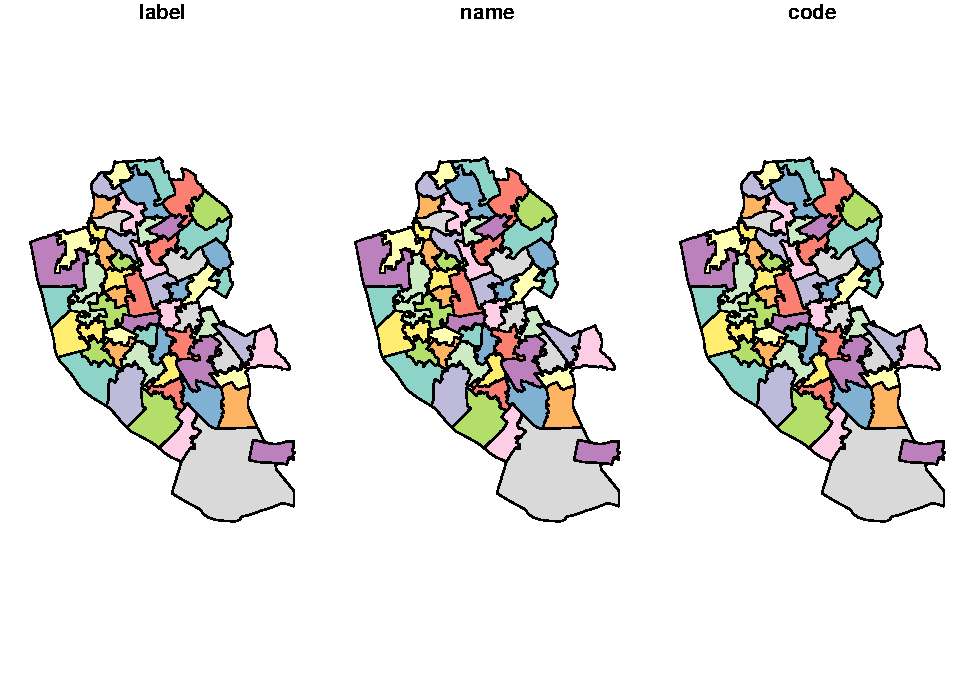
\includegraphics{Spatial-Data_files/figure-latex/unnamed-chunk-3-1.pdf}

Here we can see each MSOA's location in Liverpool. Three maps are presented - one for each column in the shapefile. This is one reason why \texttt{plot()} is not useful, since it will just plot everything. Here is it is just plotting the descriptors of each MSOA (name = name of MSOA, code/label = unique code of MSOA). You can inspect the data yourself through using \texttt{head(msoas)}.

Mapping the MSOAs themselves is a little boring, so let's join on some data. We will map COVID-19 vaccine uptake data for Liverpool - specifically the numbers of people who had receiveda vaccination between 8th December 2020 to 6th June 2021. The data are open and can be found \href{https://www.england.nhs.uk/statistics/statistical-work-areas/covid-19-vaccinations/}{here}. I have cleaned the original file and saved it in \textbf{Data} folder. The variables we have are:

\begin{itemize}
\tightlist
\item
  msoa\_code - unqiue code for each MSOA
\item
  msoa\_name - the name of each area
\item
  total\_first\_dose - the number of people who received their first COVID-19 vaccine dose
\item
  total\_second\_dose - the number of people who received two COVID-19 vaccine doses
\end{itemize}

We will now load in the data and join it onto the shapefile. To do the latter step, we will need to join on a common identifier - in this case MSOA code as it is unique and allows us to assign a one-to-one match between datasets. The \texttt{merge} command can join together files, as long as we tell R on what files to join based on (i.e., which columns are the MSOA codes found).

\begin{Shaded}
\begin{Highlighting}[]
\NormalTok{vaccine\_uptake }\OtherTok{\textless{}{-}} \FunctionTok{read.csv}\NormalTok{(}\StringTok{"./Data/msoa\_vaccine\_10June21.csv"}\NormalTok{) }\CommentTok{\# Load in vaccine uptake data}
\NormalTok{msoas }\OtherTok{\textless{}{-}} \FunctionTok{merge}\NormalTok{(msoas, vaccine\_uptake, }\AttributeTok{by.x =} \StringTok{"code"}\NormalTok{, }\AttributeTok{by.y =} \StringTok{"msoa\_code"}\NormalTok{, }\AttributeTok{all.x =} \ConstantTok{TRUE}\NormalTok{) }\CommentTok{\# Merge the vaccine uptake objects onto the msoa object, based on the columns defined (x = msoas, y = vaccine\_uptake), and do this for all observations only in the x (msoas) object}
\end{Highlighting}
\end{Shaded}

You should always quickly check whether it worked. I usually run a brief \texttt{head(msoas)} check to see if it works.

First, we will plot the number of people who have received their first dose of the COVID-19 vaccine. We will do this using \texttt{ggplot2}

\begin{Shaded}
\begin{Highlighting}[]
\FunctionTok{library}\NormalTok{(ggplot2) }\CommentTok{\# Load in package}
\NormalTok{map1 }\OtherTok{\textless{}{-}} \FunctionTok{ggplot}\NormalTok{() }\SpecialCharTok{+} \CommentTok{\# Call ggplot command}
          \FunctionTok{geom\_sf}\NormalTok{(}\AttributeTok{data =}\NormalTok{ msoas, }\FunctionTok{aes}\NormalTok{(}\AttributeTok{fill =}\NormalTok{ total\_first\_dose)) }\CommentTok{\# Using a spatial object, plot MSOAs and fill in based on number of people with first COVID{-}19 dose}
\NormalTok{map1 }\CommentTok{\# Print plot}
\end{Highlighting}
\end{Shaded}

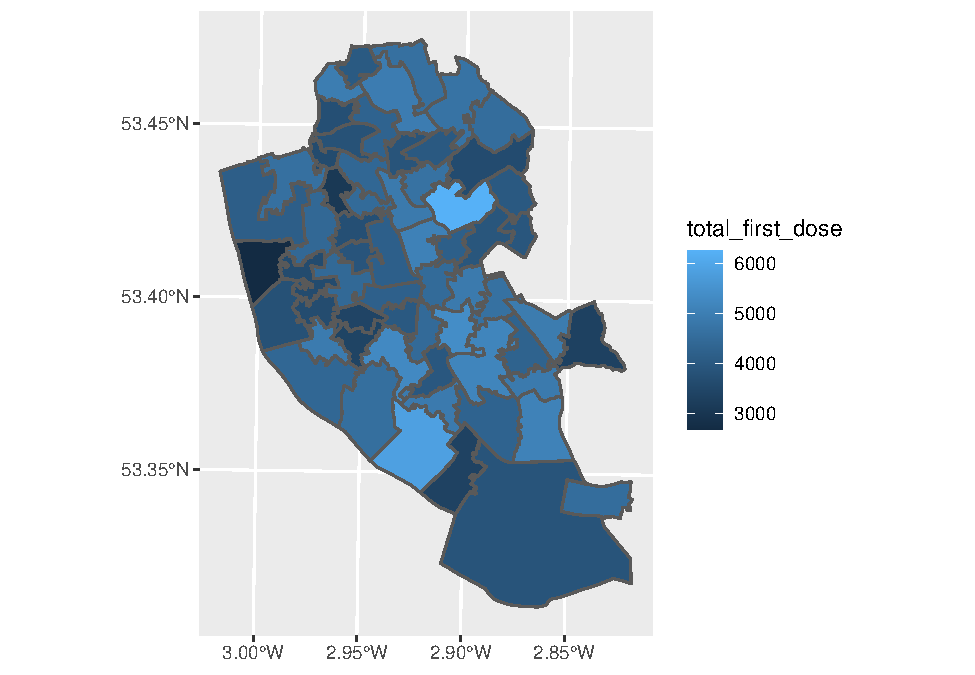
\includegraphics{Spatial-Data_files/figure-latex/unnamed-chunk-5-1.pdf}

Well done - you've made your first map! What patterns can you see? What might explain these patterns?

We can edit the map to make it nicer, how about trying the following options. Remember that \texttt{ggplot} adds each feature line-by-line, so the order of your code sometimes matters to how it is plotted.

\begin{Shaded}
\begin{Highlighting}[]
\FunctionTok{library}\NormalTok{(viridis) }\CommentTok{\# For colour blind friendly colours}
\end{Highlighting}
\end{Shaded}

\begin{verbatim}
## Loading required package: viridisLite
\end{verbatim}

\begin{Shaded}
\begin{Highlighting}[]
\NormalTok{map1 }\OtherTok{\textless{}{-}} \FunctionTok{ggplot}\NormalTok{() }\SpecialCharTok{+} \CommentTok{\# Call ggplot command}
            \FunctionTok{geom\_sf}\NormalTok{(}\AttributeTok{data =}\NormalTok{ msoas, }\FunctionTok{aes}\NormalTok{(}\AttributeTok{fill =}\NormalTok{ total\_first\_dose), }\AttributeTok{lwd =} \DecValTok{0}\NormalTok{) }\SpecialCharTok{+} \CommentTok{\# Using a spatial object, plot MSOAs and fill in based on number of people with first COVID{-}19 dose, with line width = 0 (i.e., not visible)}
            \FunctionTok{scale\_fill\_viridis\_c}\NormalTok{(}\AttributeTok{option =} \StringTok{"plasma"}\NormalTok{) }\SpecialCharTok{+} \CommentTok{\# Make colour{-}blind friendly}
            \FunctionTok{xlab}\NormalTok{(}\StringTok{"Longitude"}\NormalTok{) }\SpecialCharTok{+} \CommentTok{\# Add x{-}axis label}
            \FunctionTok{ylab}\NormalTok{(}\StringTok{"Latitude"}\NormalTok{) }\SpecialCharTok{+} \CommentTok{\# Add y{-}axis label}
            \FunctionTok{labs}\NormalTok{(}\AttributeTok{title =} \StringTok{"First dose COVID{-}19 vaccinations"}\NormalTok{, }\CommentTok{\# Add title to map}
                 \AttributeTok{fill =} \StringTok{"Frequency"}\NormalTok{) }\CommentTok{\# Edit legend title}
\NormalTok{map1 }\CommentTok{\# Print plot}
\end{Highlighting}
\end{Shaded}

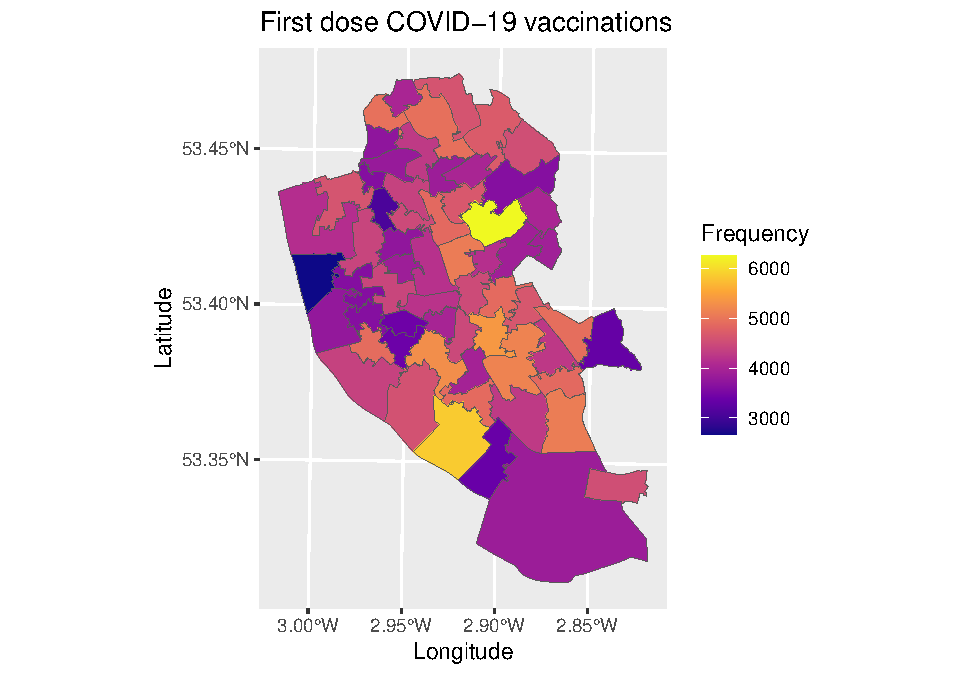
\includegraphics{Spatial-Data_files/figure-latex/unnamed-chunk-6-1.pdf}

Why not try editing some of the values above and see how it changes the aestheics of the map.

To save the map, we use the following.

\begin{Shaded}
\begin{Highlighting}[]
\FunctionTok{ggsave}\NormalTok{(}\AttributeTok{plot =}\NormalTok{ map1, }\AttributeTok{filename =} \StringTok{"./Plots/map1\_ggplot.jpeg"}\NormalTok{, }\AttributeTok{dpi =} \DecValTok{300}\NormalTok{) }\CommentTok{\# save}
\end{Highlighting}
\end{Shaded}

\begin{verbatim}
## Saving 6.5 x 4.5 in image
\end{verbatim}

We next move onto plotting using \texttt{tmap}. Here we will plot the number of people who have had two doses of the COVID-19 vaccine.

\begin{Shaded}
\begin{Highlighting}[]
\FunctionTok{library}\NormalTok{(tmap) }\CommentTok{\# Load package}
\NormalTok{map2 }\OtherTok{\textless{}{-}} \FunctionTok{tm\_shape}\NormalTok{(msoas) }\SpecialCharTok{+} \CommentTok{\# Call which spatial object}
          \FunctionTok{tm\_polygons}\NormalTok{(}\StringTok{"total\_second\_dose"}\NormalTok{) }\CommentTok{\# Which column to plot}
\NormalTok{map2 }\CommentTok{\# Print}
\end{Highlighting}
\end{Shaded}

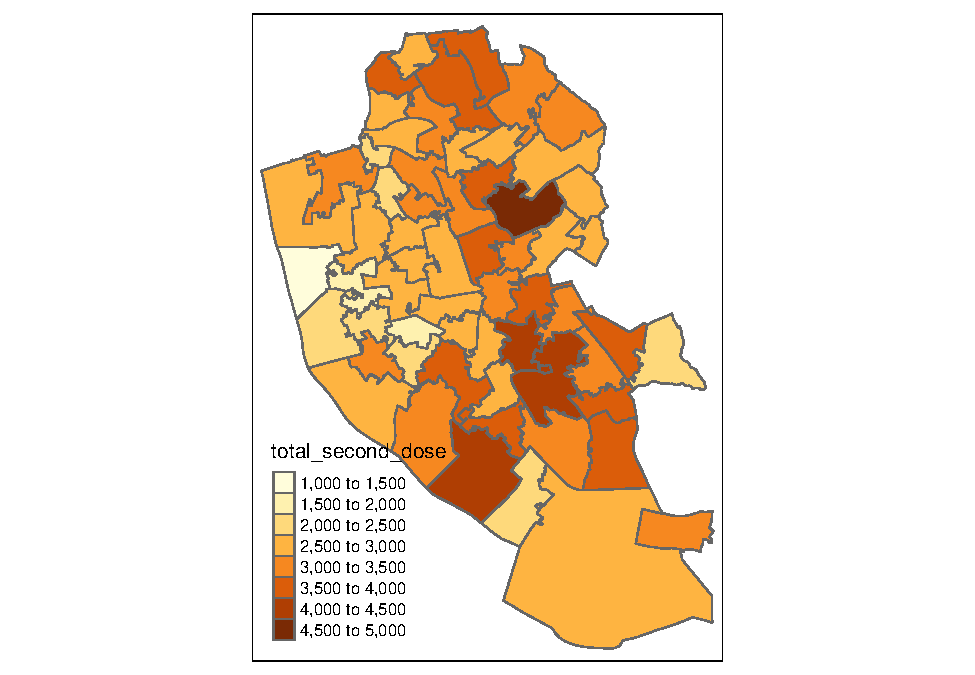
\includegraphics{Spatial-Data_files/figure-latex/unnamed-chunk-8-1.pdf}

Just as easy to use! Again, let's make the map prettier. We can also add in a few other common map conventions including a north arrow and a scale bar far easier with tmap. Note: calling viridis here can be a bit temperamental, and may need you to reload the package before running the code.

\begin{Shaded}
\begin{Highlighting}[]
\NormalTok{map2 }\OtherTok{\textless{}{-}} \FunctionTok{tm\_shape}\NormalTok{(msoas) }\SpecialCharTok{+} \CommentTok{\# Call which spatial object}
          \FunctionTok{tm\_polygons}\NormalTok{(}\StringTok{"total\_second\_dose"}\NormalTok{, }\AttributeTok{palette =} \StringTok{"viridis"}\NormalTok{, }\AttributeTok{title =} \StringTok{"Frequency"}\NormalTok{) }\SpecialCharTok{+} \CommentTok{\# Which column to plot and plot using colour blind friendly colours and edit legend to \textquotesingle{}Frequency\textquotesingle{}}
          \FunctionTok{tm\_layout}\NormalTok{(}\AttributeTok{main.title =} \StringTok{"Second dose uptake"}\NormalTok{) }\SpecialCharTok{+} \CommentTok{\# Add title}
          \FunctionTok{tm\_scale\_bar}\NormalTok{(}\AttributeTok{position =} \FunctionTok{c}\NormalTok{(}\StringTok{"right"}\NormalTok{, }\StringTok{"top"}\NormalTok{), }\AttributeTok{width =} \FloatTok{0.15}\NormalTok{) }\SpecialCharTok{+} \CommentTok{\# Add scale bar}
          \FunctionTok{tm\_compass}\NormalTok{(}\AttributeTok{position =} \FunctionTok{c}\NormalTok{(}\StringTok{"left"}\NormalTok{, }\StringTok{"top"}\NormalTok{), }\AttributeTok{size =} \DecValTok{2}\NormalTok{) }\CommentTok{\# Add north arrow}
\NormalTok{map2 }\CommentTok{\# Print}
\end{Highlighting}
\end{Shaded}

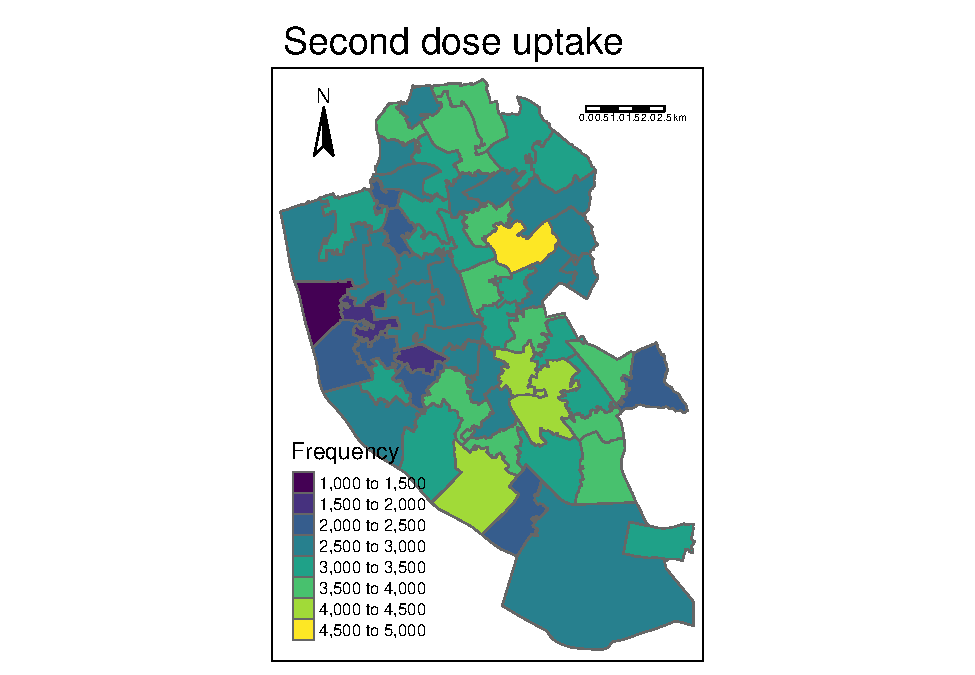
\includegraphics{Spatial-Data_files/figure-latex/unnamed-chunk-9-1.pdf}

To save the map, we do the following.

\begin{Shaded}
\begin{Highlighting}[]
\FunctionTok{tmap\_save}\NormalTok{(map2, }\AttributeTok{filename =} \StringTok{"./Plots/map2.jpeg"}\NormalTok{, }\AttributeTok{dpi =} \DecValTok{300}\NormalTok{) }\CommentTok{\# Save file}
\end{Highlighting}
\end{Shaded}

\begin{verbatim}
## Map saved to /Users/markagreen/Google Drive/Teaching/Spatial Analysis/Plots/map2.jpeg
\end{verbatim}

\begin{verbatim}
## Resolution: 1789.97 by 2463.729 pixels
\end{verbatim}

\begin{verbatim}
## Size: 5.966566 by 8.212429 inches (300 dpi)
\end{verbatim}

And there you go - just like that you have learned how to plot in R using three different packages! Easy.

\hypertarget{points}{%
\subsection{Points}\label{points}}

The next type of data we will consider are points. The area polygons we have just mapped are really a bunch of points connected by lines, so they are the building blocks of spatial data. However, they offer value by themselves for representing specific spatial positions (e.g., locations of health services).

Point data may be supplied in a spatial data format, or can just be provided as a text/csv file with a list of spatial points recorded within. The latter format can make them a little easier to handle, although since they are missing their CRS we will need to define it ourselves.

Let's have a go at plotting some points. We will stick with the COVID-19 vaccination theme here. During the initial roll-out of vaccines, Liverpool City Council funded a `vaccination bus' that could travel around Liverpool and make getting a vaccination more accessible (i.e., people could just turn up and get vaccinated there and then). Let's have a look at the areas they brought the bus to.

To load in the point locations of where the bus traveled to, we can treat the data as a standard data frame in R.

\begin{Shaded}
\begin{Highlighting}[]
\NormalTok{bus\_locations }\OtherTok{\textless{}{-}} \FunctionTok{read.csv}\NormalTok{(}\StringTok{"./Data/liverpool\_bus\_locations.csv"}\NormalTok{) }\CommentTok{\# Load data}
\end{Highlighting}
\end{Shaded}

If we use \texttt{head(bus\_locations)}, we can inspect the data. It includes the following variables:

\begin{itemize}
\tightlist
\item
  site - name of the location visited
\item
  longitude - the spatial location, as measured east-west of the Greenwich Meridian point
\item
  latitude - the spatial location, as measured north-south of the Equator
\item
  postcode - the postal address of the site (note that postcodes are not unique and may represent 15 households)
\item
  location - latitude and longitude combined into a single geometry point
\end{itemize}

The data is currently stored in a data frame format. We need to tell R that it is actually spatial data, so that it can plot it as such. \texttt{sf} can help us here.

\begin{Shaded}
\begin{Highlighting}[]
\CommentTok{\# Convert to spatial data frame}
\NormalTok{bus\_locations\_sp }\OtherTok{\textless{}{-}}\NormalTok{ bus\_locations }\SpecialCharTok{\%\textgreater{}\%} \CommentTok{\# For object (bus locations)}
  \FunctionTok{st\_as\_sf}\NormalTok{(}\AttributeTok{coords =} \FunctionTok{c}\NormalTok{(}\StringTok{"longitude"}\NormalTok{, }\StringTok{"latitude"}\NormalTok{)) }\SpecialCharTok{\%\textgreater{}\%} \CommentTok{\# Define as spatial object and identify which columns tell us the position of points}
  \FunctionTok{st\_set\_crs}\NormalTok{(}\DecValTok{4326}\NormalTok{) }\CommentTok{\# Set CRS}
\end{Highlighting}
\end{Shaded}

Let's look at where these points are located. First, we will use \texttt{ggplot2}.

\begin{Shaded}
\begin{Highlighting}[]
\NormalTok{map3 }\OtherTok{\textless{}{-}} \FunctionTok{ggplot}\NormalTok{() }\SpecialCharTok{+} \CommentTok{\# Call ggplot command}
            \FunctionTok{geom\_sf}\NormalTok{(}\AttributeTok{data =}\NormalTok{ bus\_locations\_sp, }\AttributeTok{colour =} \StringTok{"green"}\NormalTok{) }\SpecialCharTok{+} \CommentTok{\# Plot points as green dots}
            \FunctionTok{xlab}\NormalTok{(}\StringTok{"Longitude"}\NormalTok{) }\SpecialCharTok{+} \CommentTok{\# Add x{-}axis label}
            \FunctionTok{ylab}\NormalTok{(}\StringTok{"Latitude"}\NormalTok{) }\SpecialCharTok{+} \CommentTok{\# Add y{-}axis label}
            \FunctionTok{labs}\NormalTok{(}\AttributeTok{title =} \StringTok{"Location of vaccine bus"}\NormalTok{) }\CommentTok{\# Edit legend title}
\NormalTok{map3 }\CommentTok{\# Print plot}
\end{Highlighting}
\end{Shaded}

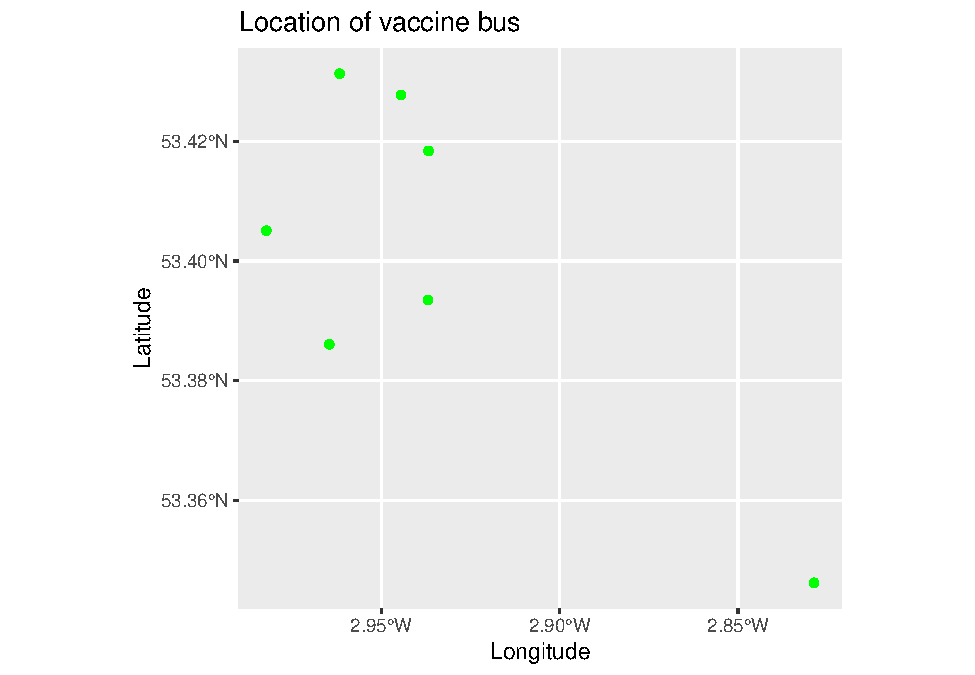
\includegraphics{Spatial-Data_files/figure-latex/unnamed-chunk-13-1.pdf}

Hmmmm, that is not particularly useful by itself. Let's add these points to the map of vaccine uptake that we made earlier. This will help us tell if the locations were targeted at areas with low or high uptake. Note that we call the points after the area data, since \texttt{ggplot2} builds the plot sequentially, this helps to ensure the points are plotted on top of the area data.

\begin{Shaded}
\begin{Highlighting}[]
\NormalTok{map3 }\OtherTok{\textless{}{-}} \FunctionTok{ggplot}\NormalTok{() }\SpecialCharTok{+} \CommentTok{\# Call ggplot command}
            \FunctionTok{geom\_sf}\NormalTok{(}\AttributeTok{data =}\NormalTok{ msoas, }\FunctionTok{aes}\NormalTok{(}\AttributeTok{fill =}\NormalTok{ total\_first\_dose), }\AttributeTok{lwd =} \DecValTok{0}\NormalTok{) }\SpecialCharTok{+} \CommentTok{\# Plot vaccine uptake (1st dose)}
            \FunctionTok{scale\_fill\_viridis\_c}\NormalTok{(}\AttributeTok{option =} \StringTok{"plasma"}\NormalTok{) }\SpecialCharTok{+} \CommentTok{\# Make colour{-}blind friendly}
            \FunctionTok{geom\_sf}\NormalTok{(}\AttributeTok{data =}\NormalTok{ bus\_locations\_sp, }\AttributeTok{colour =} \StringTok{"green"}\NormalTok{) }\SpecialCharTok{+} \CommentTok{\# Plot points as green dots}
            \FunctionTok{xlab}\NormalTok{(}\StringTok{"Longitude"}\NormalTok{) }\SpecialCharTok{+} \CommentTok{\# Add x{-}axis label}
            \FunctionTok{ylab}\NormalTok{(}\StringTok{"Latitude"}\NormalTok{) }\SpecialCharTok{+} \CommentTok{\# Add y{-}axis label}
            \FunctionTok{labs}\NormalTok{(}\AttributeTok{title =} \StringTok{"First dose COVID{-}19 vaccinations"}\NormalTok{, }\CommentTok{\# Add title to map}
                 \AttributeTok{caption =} \StringTok{"Green dots are locations of vaccine bus"}\NormalTok{, }\CommentTok{\# Add description to bottom of map (alternatively could place as subtitle = "" too)}
                 \AttributeTok{fill =} \StringTok{"Frequency"}\NormalTok{) }\CommentTok{\# Edit legend title}
\NormalTok{map3 }\CommentTok{\# Print plot}
\end{Highlighting}
\end{Shaded}

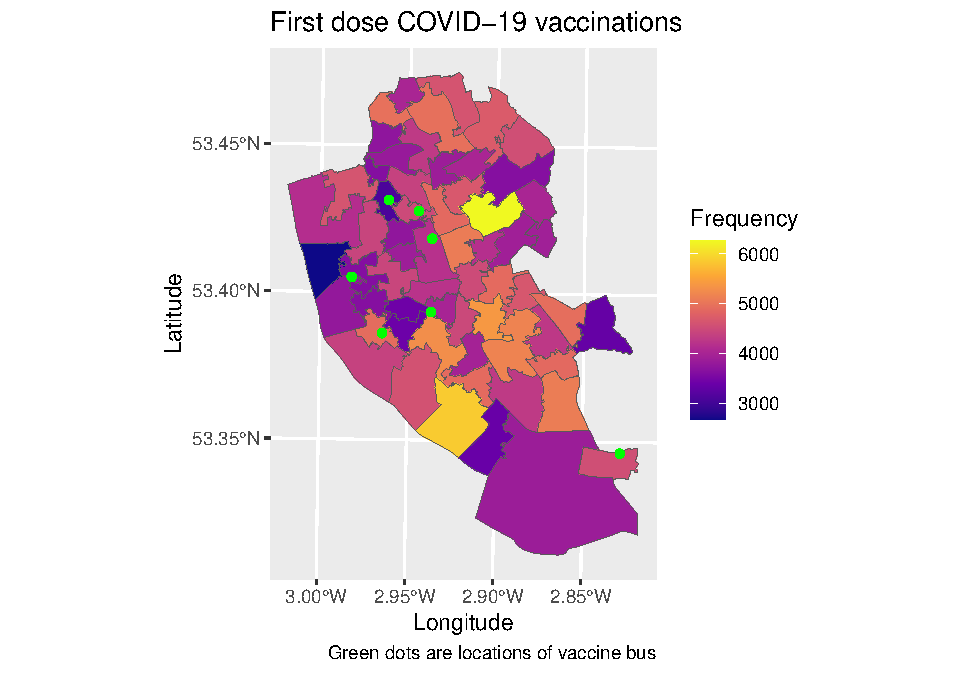
\includegraphics{Spatial-Data_files/figure-latex/unnamed-chunk-14-1.pdf}

How useful do you think the vaccine bus locations are? Do you think this approach is helpful? How might you improve or better target their locations?

We can do the same using \texttt{tmap} too. We next recreate the same map from earlier (2nd dose uptake) and compare it to vaccine bus locations.

\begin{Shaded}
\begin{Highlighting}[]
\NormalTok{map4 }\OtherTok{\textless{}{-}} \FunctionTok{tm\_shape}\NormalTok{(msoas) }\SpecialCharTok{+} \CommentTok{\# Call area data object}
          \FunctionTok{tm\_polygons}\NormalTok{(}\StringTok{"total\_second\_dose"}\NormalTok{, }\AttributeTok{palette =} \StringTok{"viridis"}\NormalTok{, }\AttributeTok{title =} \StringTok{"Frequency"}\NormalTok{) }\SpecialCharTok{+} \CommentTok{\# Which column to plot and plot using colour blind friendly colours and edit legend to \textquotesingle{}Frequency\textquotesingle{}}
        \FunctionTok{tm\_shape}\NormalTok{(bus\_locations\_sp) }\SpecialCharTok{+} \CommentTok{\# Call spatial points}
          \FunctionTok{tm\_dots}\NormalTok{(}\AttributeTok{size =} \FloatTok{0.5}\NormalTok{) }\SpecialCharTok{+} \CommentTok{\# Plot points (cal call specific variable here too)}
        \FunctionTok{tm\_layout}\NormalTok{(}\AttributeTok{main.title =} \StringTok{"Second dose uptake"}\NormalTok{) }\SpecialCharTok{+} \CommentTok{\# Add title}
        \FunctionTok{tm\_scale\_bar}\NormalTok{(}\AttributeTok{position =} \FunctionTok{c}\NormalTok{(}\StringTok{"right"}\NormalTok{, }\StringTok{"top"}\NormalTok{), }\AttributeTok{width =} \FloatTok{0.15}\NormalTok{) }\SpecialCharTok{+} \CommentTok{\# Add scale bar}
        \FunctionTok{tm\_compass}\NormalTok{(}\AttributeTok{position =} \FunctionTok{c}\NormalTok{(}\StringTok{"left"}\NormalTok{, }\StringTok{"top"}\NormalTok{), }\AttributeTok{size =} \DecValTok{2}\NormalTok{) }\CommentTok{\# Add north arrow}
\NormalTok{map4 }\CommentTok{\# Print}
\end{Highlighting}
\end{Shaded}

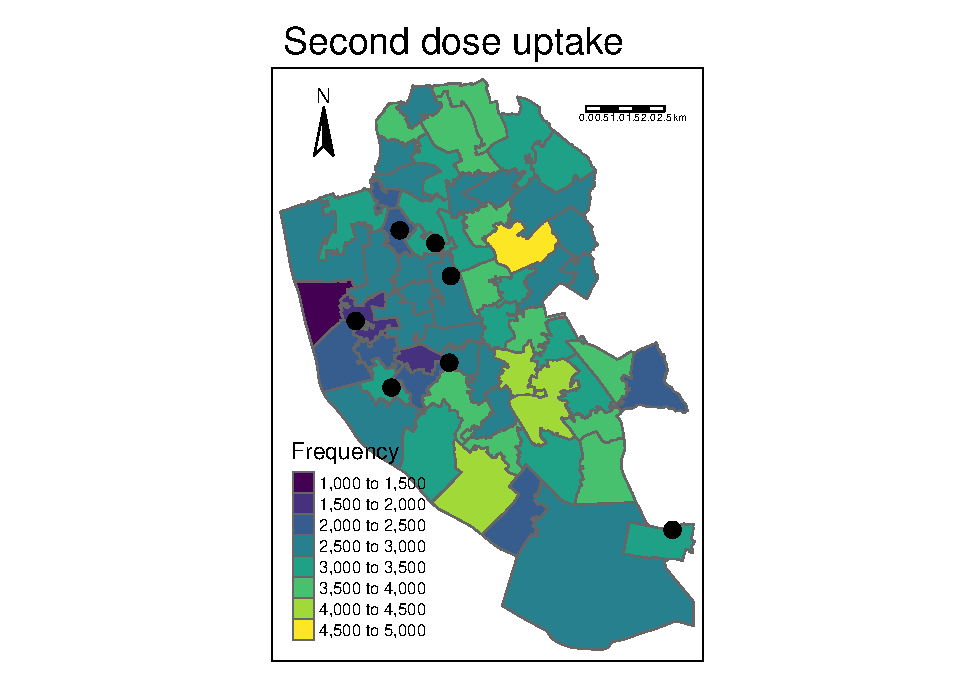
\includegraphics{Spatial-Data_files/figure-latex/unnamed-chunk-15-1.pdf}

Here, we have to call two spatial objects and then tell \texttt{tmap} what to plot, which is a different approach to the \texttt{ggplot2} code.

\hypertarget{interactive-maps}{%
\section{Interactive maps}\label{interactive-maps}}

So far we have created `static' maps. They are static in the sense that they do not move or change, which is important for print media (i.e., those printed in articles). It can be preferable to create interactive plots where users can actively engage with data.

\texttt{ggplot2} does not natively allow for interactive maps, however \texttt{tmap} does. All we have to do is tell \texttt{tmap} we want to create an interactive and clickable map, and then run our code from earlier.

\begin{Shaded}
\begin{Highlighting}[]
\FunctionTok{tmap\_mode}\NormalTok{(}\StringTok{"view"}\NormalTok{) }\CommentTok{\# Set tmap to interactive plotting mode}
\end{Highlighting}
\end{Shaded}

\begin{verbatim}
## tmap mode set to interactive viewing
\end{verbatim}

\begin{Shaded}
\begin{Highlighting}[]
\NormalTok{map4 }\CommentTok{\# Plot map object}
\end{Highlighting}
\end{Shaded}

\begin{verbatim}
## Compass not supported in view mode.
\end{verbatim}

\begin{verbatim}
## Scale bar width set to 100 pixels
\end{verbatim}

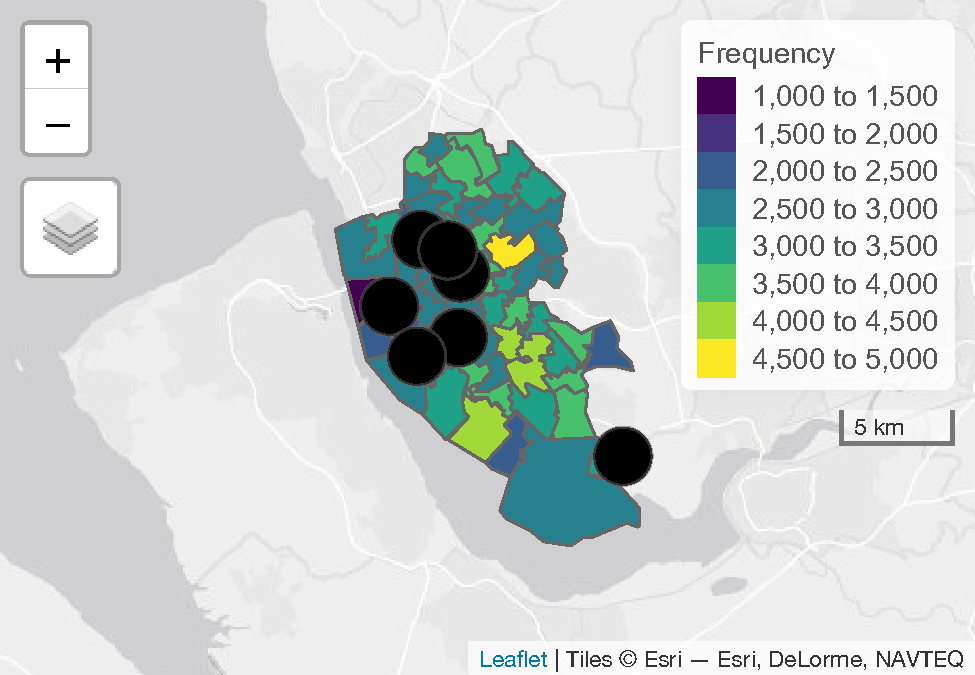
\includegraphics{Spatial-Data_files/figure-latex/unnamed-chunk-16-1.pdf}

\begin{Shaded}
\begin{Highlighting}[]
\CommentTok{\# Alternatively, you can just run the code and it will create the interactive map on the fly {-} try running the following:}
\CommentTok{\# tm\_shape(msoas) + \# Call which spatial object}
\CommentTok{\#   tm\_polygons("total\_second\_dose", palette = "RdYlBu") \# Which column to plot, and change colour}
\end{Highlighting}
\end{Shaded}

If you hover over points or areas, you will see there is a description of what they are (based on first column in the dataset, although this can be changed). You can also change the base map by clicking on the layers box to the left. This is also useful as you can plot multiple layers at once and switch between them.

If you want to make static maps again, you will need to tell \texttt{tmap} this through running the following code \texttt{tmap\_mode("plot")}.

We can also save these interactive maps as standalone html files that can be shared.

\begin{Shaded}
\begin{Highlighting}[]
\FunctionTok{tmap\_save}\NormalTok{(map4, }\AttributeTok{filename =} \StringTok{"./Plots/vaccine\_bus\_interactive.html"}\NormalTok{) }\CommentTok{\# Save}
\end{Highlighting}
\end{Shaded}

\begin{verbatim}
## Compass not supported in view mode.
\end{verbatim}

\begin{verbatim}
## Scale bar width set to 100 pixels
\end{verbatim}

\begin{verbatim}
## Interactive map saved to ./Plots/vaccine_bus_interactive.html
\end{verbatim}

We can edit the basemaps presented here to a range of options. A couple of my favourites include:

\begin{itemize}
\tightlist
\item
  Carto as basemap for tiles, rather than default of ESRI
\item
  Stamen which is just pretty
\item
  OpenStreetMap is always worth a shout
\end{itemize}

Below is some code to try these styles, but you can inspect the range of designs and options \href{https://leaflet-extras.github.io/leaflet-providers/preview/}{here}

\begin{Shaded}
\begin{Highlighting}[]
\CommentTok{\# \# Carto {-} light}
\CommentTok{\# tm\_basemap(leaflet::providers$CartoDB.PositronNoLabels, group = "CartoDB basemap") + \# Plot Carto basemap}
\CommentTok{\#     tm\_shape(msoas) + \# Select MSOA object}
\CommentTok{\#     tm\_polygons("total\_second\_dose", palette = "RdYlBu") + \# Plot vaccine uptake (2nd dose)}
\CommentTok{\#     tm\_tiles(leaflet::providers$CartoDB.PositronOnlyLabels, group = "CartoDB labels") \# Plot place name labels}

\CommentTok{\# \# Carto {-} dark}
\CommentTok{\# tm\_basemap(leaflet::providers$CartoDB.DarkMatter) + \# Plot Carto basemap}
\CommentTok{\#     tm\_shape(msoas) + \# Select MSOA object}
\CommentTok{\#     tm\_polygons("total\_second\_dose", palette = "RdYlBu")}

\CommentTok{\# \# Stamen}
\CommentTok{\# tm\_basemap("Stamen.Watercolor") + \# Add Stamen as basemap}
\CommentTok{\#     tm\_shape(msoas) + \# Select MSOA object}
\CommentTok{\#     tm\_polygons("total\_second\_dose", palette = "RdYlBu") + \# Plot vaccine uptake (2nd dose)}
\CommentTok{\#     tm\_tiles("Stamen.TonerLabels") \# Adds labels for areas (e.g., place names)}

\CommentTok{\# \# OpenStreetMap}
\CommentTok{\# tm\_basemap("OpenStreetMap.HOT") + \# Plot basemap}
\CommentTok{\#     tm\_shape(msoas) + \# Select MSOA object}
\CommentTok{\#     tm\_polygons("total\_second\_dose", palette = "RdYlBu")}
\end{Highlighting}
\end{Shaded}

The eagled-eye of you may have noticed that this technology is enabled through something called \texttt{leaflet}. We can actually create interactive maps using \texttt{leaflet} directly, which gives greater flexibility and control (even if the code is longer and more difficult). Let's give it a go!

\begin{Shaded}
\begin{Highlighting}[]
\CommentTok{\# Load package}
\FunctionTok{library}\NormalTok{(leaflet)}

\CommentTok{\# Transform the CRS to match WGS84 format for leaflet}
\NormalTok{msoas }\OtherTok{\textless{}{-}} \FunctionTok{st\_transform}\NormalTok{(msoas, }\DecValTok{4326}\NormalTok{)}

\CommentTok{\# Define parameters for colours for mapping}
\NormalTok{pal }\OtherTok{\textless{}{-}} \FunctionTok{colorNumeric}\NormalTok{(}\FunctionTok{viridis\_pal}\NormalTok{(}\AttributeTok{option =} \StringTok{"viridis"}\NormalTok{)(}\DecValTok{2}\NormalTok{), }\AttributeTok{domain =} \FunctionTok{c}\NormalTok{(}\DecValTok{0}\NormalTok{, }\DecValTok{5000}\NormalTok{)) }\CommentTok{\# Set doman as min/max}

\CommentTok{\# Plot}
\FunctionTok{leaflet}\NormalTok{() }\SpecialCharTok{\%\textgreater{}\%}
  \CommentTok{\# Add area data on vaccine uptake populations}
  \FunctionTok{addPolygons}\NormalTok{(}\AttributeTok{data =}\NormalTok{ msoas, }\CommentTok{\# Define data}
              \AttributeTok{fillColor =} \SpecialCharTok{\textasciitilde{}}\FunctionTok{pal}\NormalTok{(total\_second\_dose), }\CommentTok{\# Specify the variable to be plotted, with pal representing the colours to plot}
              \AttributeTok{weight =} \DecValTok{0}\NormalTok{, }\CommentTok{\# Define how thick the lines will be }
              \AttributeTok{opacity =} \DecValTok{0}\NormalTok{, }\CommentTok{\# How see through we want the lines to be (0\%)}
              \AttributeTok{fillOpacity =} \FloatTok{0.5}\NormalTok{) }\SpecialCharTok{\%\textgreater{}\%} \CommentTok{\# How see through we want areas coloured in to be (50\%)}
  \CommentTok{\# Add bus locations in}
  \FunctionTok{addCircleMarkers}\NormalTok{(}\AttributeTok{data =}\NormalTok{ bus\_locations\_sp, }\CommentTok{\# Define data}
                   \AttributeTok{radius =} \DecValTok{1}\NormalTok{, }\CommentTok{\# Only plot immediate location}
                   \AttributeTok{color =} \StringTok{"red"}\NormalTok{) }\SpecialCharTok{\%\textgreater{}\%} \CommentTok{\# Select colour to plot}
  \FunctionTok{addProviderTiles}\NormalTok{(}\StringTok{"CartoDB.Positron"}\NormalTok{) }\CommentTok{\# Define base map, here as Carto}
\end{Highlighting}
\end{Shaded}

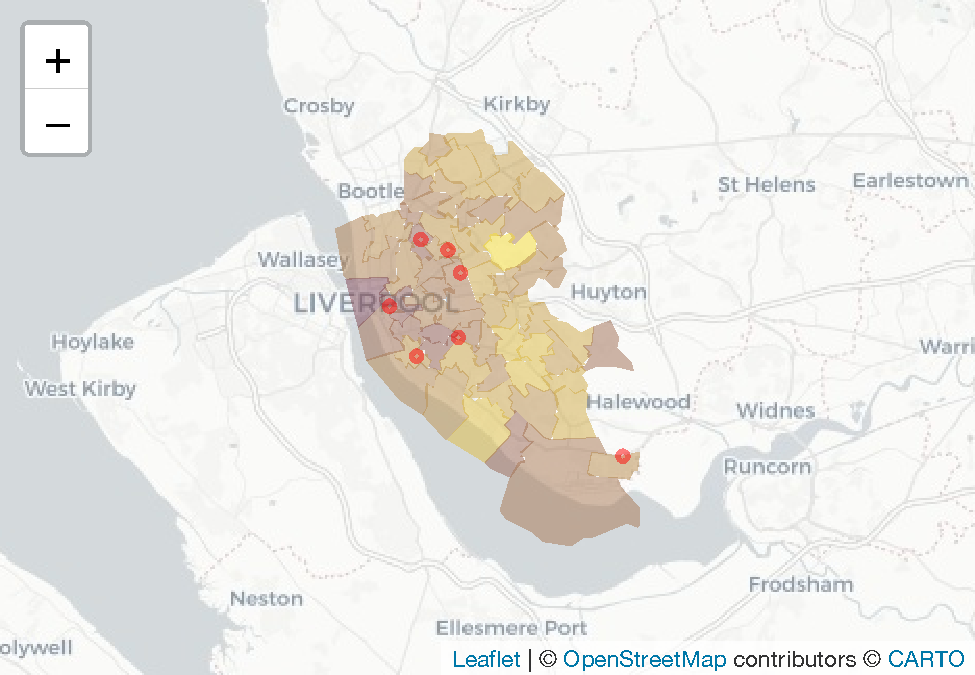
\includegraphics{Spatial-Data_files/figure-latex/unnamed-chunk-19-1.pdf}

\hypertarget{summary}{%
\section{Summary}\label{summary}}

Well done! You have learned how to visualise spatial data, make professionally looking maps, and think about how to effectively present information in static and interactive ways. In the next section, we will consider how to apply this spatial way of presenting data into more formal approaches of analysis.

\hypertarget{cluster}{%
\chapter{Cluster analysis}\label{cluster}}

In this section, we will introduce how we can analyse spatial data including identifying clustering of data. The lecture slides for this practical can be found \href{}{here}. A PDF version of the practical can be found \href{}{here}. We define clustering here as where data (locations, or high/low values) are geographically concentrated in particular areas and not evenly spread out.

\hypertarget{point-data}{%
\section{Point data}\label{point-data}}

There are numerous point-based methods including clustering algorithms, spatial scan metrics, and count regression models that we could talk about here - too much to cover in this section. Instead, we will focus on descriptive techniques for displaying point-based data.

\hypertarget{spatial-histograms}{%
\subsection{Spatial histograms}\label{spatial-histograms}}

One of the first steps we might take in trying to see if our point data are spatially clustered is by plotting their locations. This may be important if we are looking at the locations of disease cases or outbreaks, allowing us to make inferences about clustering of diseases and the reasons behind this. In the example here, we will look at food outlets in Liverpool to assess if they are geographically concentrated in particular areas of Liverpool.

We will first load in the data on locations of food outlets. The data are taken from the Food Standards Agency website \href{https://ratings.food.gov.uk/}{here} and are open data. While there are too many columns to describe here, it is worth familiarising yourself with all these columns using \texttt{head(food\_outlets)} first. The key variables we will be using are:

\begin{itemize}
\tightlist
\item
  Geocode.Longitude - longitude for location of premises
\item
  Geocode.Latitude - latitude for location of premises
\end{itemize}

We also will load in the boundary shapefile for Liverpool here, to help provide a background for our points.

\begin{Shaded}
\begin{Highlighting}[]
\FunctionTok{library}\NormalTok{(sf) }\CommentTok{\# Load package}

\CommentTok{\# Load food outlets data}
\NormalTok{food\_outlets }\OtherTok{\textless{}{-}} \FunctionTok{read.csv}\NormalTok{(}\StringTok{"./Data/liverpool\_food\_outlets.csv"}\NormalTok{) }\CommentTok{\# Load data}
\NormalTok{food\_outlets }\OtherTok{\textless{}{-}}\NormalTok{ food\_outlets[}\SpecialCharTok{!}\FunctionTok{is.na}\NormalTok{(food\_outlets}\SpecialCharTok{$}\NormalTok{Geocode.Latitude),] }\CommentTok{\# Drop missing co{-}ordinates (e.g., burger vans that have no fixed position) since cannot plot them}

\CommentTok{\# Convert to spatial points data frame}
\NormalTok{food\_outlets\_sp }\OtherTok{\textless{}{-}}\NormalTok{ food\_outlets }\SpecialCharTok{\%\textgreater{}\%} \CommentTok{\# For object}
  \FunctionTok{st\_as\_sf}\NormalTok{(}\AttributeTok{coords =} \FunctionTok{c}\NormalTok{(}\StringTok{"Geocode.Longitude"}\NormalTok{, }\StringTok{"Geocode.Latitude"}\NormalTok{)) }\SpecialCharTok{\%\textgreater{}\%} \CommentTok{\# Define as spatial object and identify which columns tell us the position of points}
  \FunctionTok{st\_set\_crs}\NormalTok{(}\DecValTok{4326}\NormalTok{) }\CommentTok{\# Set CRS}

\CommentTok{\# Load Liverpool outline}
\NormalTok{liverpool }\OtherTok{\textless{}{-}} \FunctionTok{read\_sf}\NormalTok{(}\StringTok{"./Shapefiles/Liverpool\_LAD/england\_lad\_2011.shp"}\NormalTok{)  }\CommentTok{\# Load in shapefile}
\NormalTok{liverpool }\OtherTok{\textless{}{-}} \FunctionTok{st\_transform}\NormalTok{(liverpool, }\DecValTok{4326}\NormalTok{) }\CommentTok{\# Reproject to same as long/lat format}
\end{Highlighting}
\end{Shaded}

Ok, with the data loaded in, we can now map the points.

\begin{Shaded}
\begin{Highlighting}[]
\FunctionTok{library}\NormalTok{(ggplot2) }\CommentTok{\# Load package}
\NormalTok{map1 }\OtherTok{\textless{}{-}} \FunctionTok{ggplot}\NormalTok{() }\SpecialCharTok{+} \CommentTok{\# Call ggplot command}
  \FunctionTok{geom\_sf}\NormalTok{(}\AttributeTok{data =}\NormalTok{ liverpool) }\SpecialCharTok{+} \CommentTok{\# Load liverpool outline}
  \FunctionTok{geom\_sf}\NormalTok{(}\AttributeTok{data =}\NormalTok{ food\_outlets\_sp) }\SpecialCharTok{+} \CommentTok{\# Plot food outlet as dots}
  \FunctionTok{xlab}\NormalTok{(}\StringTok{"Longitude"}\NormalTok{) }\SpecialCharTok{+} \CommentTok{\# Add x{-}axis label}
  \FunctionTok{ylab}\NormalTok{(}\StringTok{"Latitude"}\NormalTok{) }\SpecialCharTok{+} \CommentTok{\# Add y{-}axis label}
  \FunctionTok{labs}\NormalTok{(}\AttributeTok{title =} \StringTok{"Food outlets in Liverpool"}\NormalTok{) }\CommentTok{\# Edit plot title}
\NormalTok{map1 }\CommentTok{\# Print plot}
\end{Highlighting}
\end{Shaded}

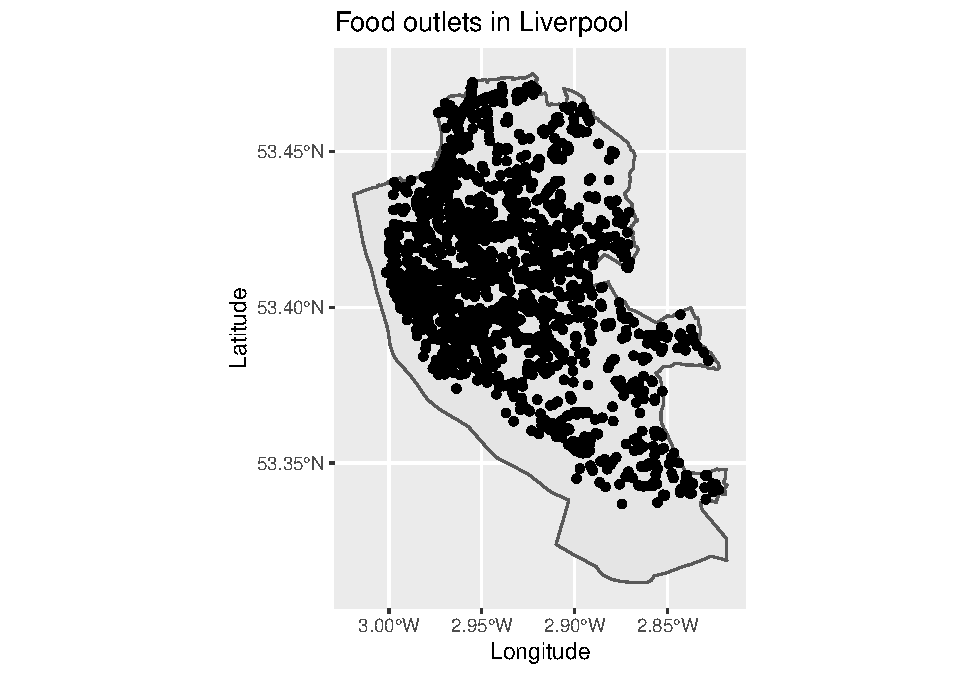
\includegraphics{Spatial-Data_files/figure-latex/unnamed-chunk-21-1.pdf}

Hmmmm, you may see there is an issue with interpretating this plot - many of the plots overlap each other making it difficult to determine underlying patterns. We therefore need a way of summarising this information.

Histograms are useful plots for examining the distribution of single variables - we can apply them spatially by creating \textbf{spatial histograms}. To do this, we need to create spatial \textbf{bins} and then count how many points are in each of those bins. We use this binning approach when producing histograms for single variables (e.g., counting how many points exist at each value of a variable) and just extend it here for each x,y position on a map. I recommend using a \textbf{hex} approach, since hexagons can minimise visual artefacts that can be created through other shapes.

\begin{Shaded}
\begin{Highlighting}[]
\FunctionTok{library}\NormalTok{(viridis) }\CommentTok{\# Load package}
\NormalTok{map2 }\OtherTok{\textless{}{-}} \FunctionTok{ggplot}\NormalTok{() }\SpecialCharTok{+} \CommentTok{\# Call ggplot2}
  \FunctionTok{geom\_sf}\NormalTok{(}\AttributeTok{data =}\NormalTok{ liverpool) }\SpecialCharTok{+} \CommentTok{\# Load liverpool outline}
  \FunctionTok{geom\_hex}\NormalTok{(}\AttributeTok{data =}\NormalTok{ food\_outlets, }\FunctionTok{aes}\NormalTok{(}\AttributeTok{x =}\NormalTok{ Geocode.Longitude, }\AttributeTok{y =}\NormalTok{ Geocode.Latitude)) }\SpecialCharTok{+} \CommentTok{\# Define data to be plotted}
  \FunctionTok{scale\_fill\_viridis}\NormalTok{() }\SpecialCharTok{+} \CommentTok{\# Make colour blind friendly}
  \FunctionTok{xlab}\NormalTok{(}\StringTok{"Longitude"}\NormalTok{) }\SpecialCharTok{+} \CommentTok{\# Add x{-}axis label}
  \FunctionTok{ylab}\NormalTok{(}\StringTok{"Latitude"}\NormalTok{) }\SpecialCharTok{+} \CommentTok{\# Add y{-}axis label}
  \FunctionTok{labs}\NormalTok{(}\AttributeTok{title =} \StringTok{"Food outlets in Liverpool"}\NormalTok{) }\CommentTok{\# Edit plot title}
\NormalTok{map2}
\end{Highlighting}
\end{Shaded}

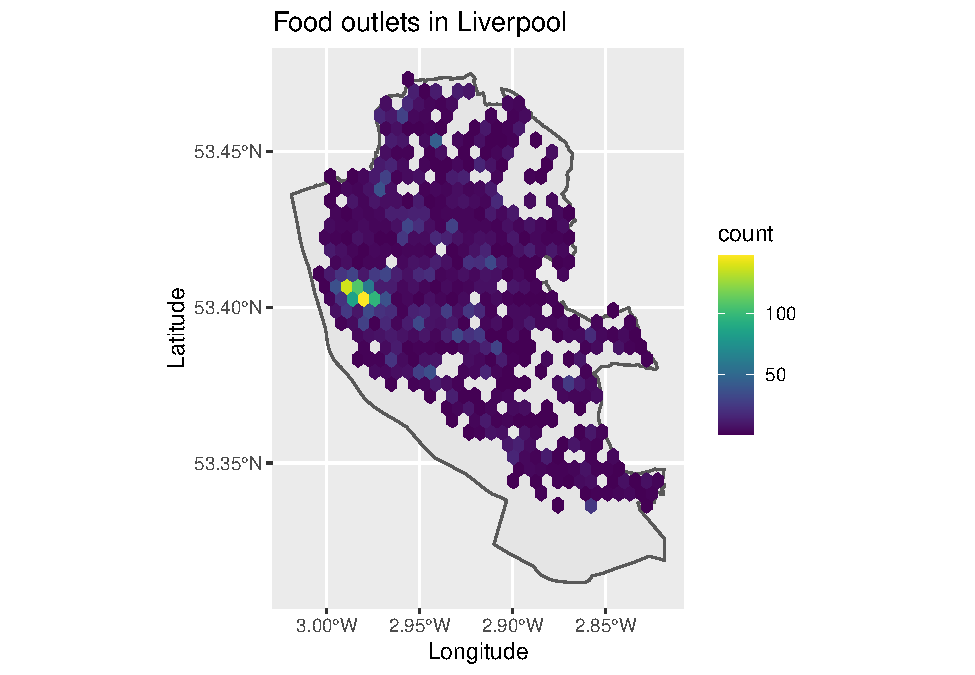
\includegraphics{Spatial-Data_files/figure-latex/unnamed-chunk-22-1.pdf}

We can now see the clustering of points in the city centre, with food outlets covering most of the city.

\hypertarget{kernal-density-estimation}{%
\subsection{Kernal Density Estimation}\label{kernal-density-estimation}}

An alternative approach might be to use \textbf{Kernal Density Estimation (KDE)} which can create a continuous surface for the density/clustering of points. This avoids the limitation of spatial histograms through creating a single map with no boundaries, rather than splitting up areas into arbitrary bins. KDE or density plots are often used as alternative to standard histograms.

Here we are measuring the intensity or density of points for a given location. We can run these analyses in \texttt{ggplot2} using the \texttt{stat\_density2d\_filled} command.

\begin{Shaded}
\begin{Highlighting}[]
\NormalTok{map3 }\OtherTok{\textless{}{-}} \FunctionTok{ggplot}\NormalTok{() }\SpecialCharTok{+} \CommentTok{\# Call ggplot2}
    \FunctionTok{geom\_sf}\NormalTok{(}\AttributeTok{data =}\NormalTok{ liverpool) }\SpecialCharTok{+} \CommentTok{\# Load liverpool outline}
    \FunctionTok{stat\_density2d\_filled}\NormalTok{( }\CommentTok{\# Call KDE or smoothed density plot}
        \AttributeTok{data =}\NormalTok{ food\_outlets, }\FunctionTok{aes}\NormalTok{(}\AttributeTok{x =}\NormalTok{ Geocode.Longitude, }\AttributeTok{y =}\NormalTok{ Geocode.Latitude, }\CommentTok{\# Define data and locations}
                                 \AttributeTok{fill =}\NormalTok{ ..level..,}\AttributeTok{alpha=}\NormalTok{..level..), }\CommentTok{\# Set paramters for colouring in values}
        \AttributeTok{n =} \DecValTok{100} \CommentTok{\# Modify and see how changes the map (is number of neighbours to derive clustering from)}
\NormalTok{    ) }\SpecialCharTok{+}
    \FunctionTok{scale\_color\_viridis}\NormalTok{() }\SpecialCharTok{+} \CommentTok{\# Make colour blind friendly}
    \FunctionTok{xlab}\NormalTok{(}\StringTok{"Longitude"}\NormalTok{) }\SpecialCharTok{+} \CommentTok{\# Add x{-}axis label}
    \FunctionTok{ylab}\NormalTok{(}\StringTok{"Latitude"}\NormalTok{) }\SpecialCharTok{+} \CommentTok{\# Add y{-}axis label}
    \FunctionTok{labs}\NormalTok{(}\AttributeTok{title =} \StringTok{"Food outlets in Liverpool"}\NormalTok{) }\CommentTok{\# Edit plot title}
\NormalTok{map3}
\end{Highlighting}
\end{Shaded}

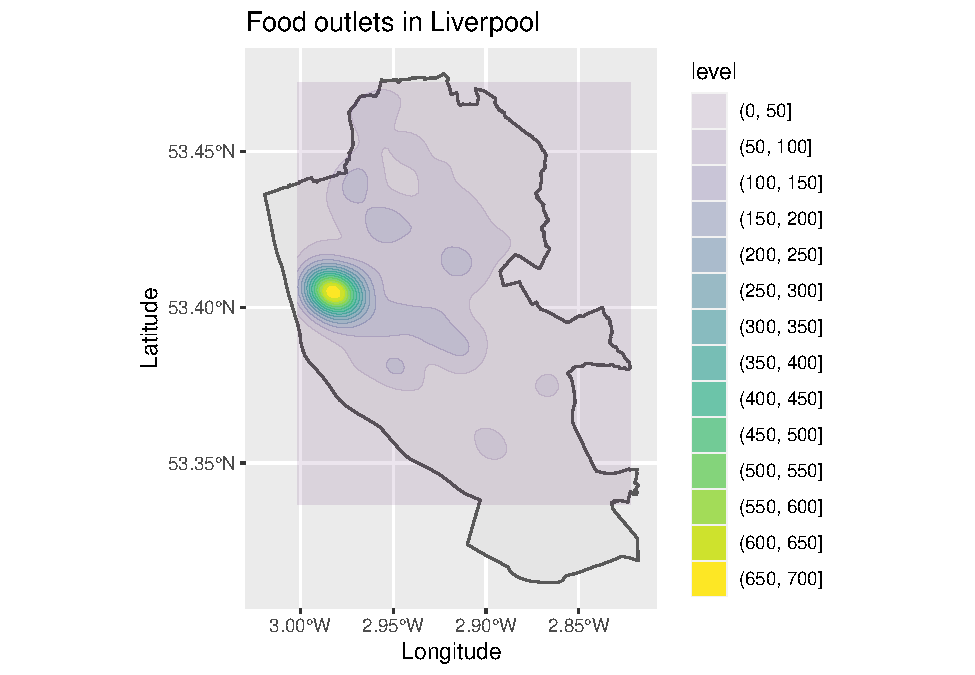
\includegraphics{Spatial-Data_files/figure-latex/unnamed-chunk-23-1.pdf}

The resulting map is similar to the hexmap earlier, but we now have one contiguous and single surface for the data. It is worth playing about with the number of neighbours to examine how the algorithm changes the resulting map. Sometimes these are called `heatmaps'.

\hypertarget{spatial-interpolation}{%
\subsection{Spatial interpolation}\label{spatial-interpolation}}

Sometimes the point data that we have contain values or variables that tell us information about them. Here we might be interested in values themselves, rather than the clustering of their locations. We therefore need a different approach here.

To demonstrate how to visualise and extract some value here, we will use a new dataset. The data can be found \href{https://qof.digital.nhs.uk/}{here} and are open data. I have done some additional cleaning on the data and extracted their spatial locations to save us time. There is active debate over how useful these data are, but they provide a helpful case study. The variables in the dataset are:

\begin{itemize}
\tightlist
\item
  pcn\_code - unique code for the primary care network (groups of GP practices/surgeries)
\item
  pcn\_name - name for primary care network
\item
  gp\_code - unique code for GP surgery
\item
  gp\_name - name of GP surgery
\item
  chronic\_heart\_disease\_percent - estimated percentage of people at the surgery who have chronic heart disease
\item
  obese\_percent - estimated percentage of people who are defined as obese
\item
  postcode - postcode for GP surgery
\item
  longitude - longitude location
\item
  latitude - latitude location
\end{itemize}

Let's load in these data.

\begin{Shaded}
\begin{Highlighting}[]
\CommentTok{\# Load data}
\NormalTok{gp\_locations }\OtherTok{\textless{}{-}} \FunctionTok{read.csv}\NormalTok{(}\StringTok{"./Data/gp\_qof\_1920.csv"}\NormalTok{)}

\CommentTok{\# Convert to spatial points data frame}
\NormalTok{gp\_locations\_sp }\OtherTok{\textless{}{-}}\NormalTok{ gp\_locations }\SpecialCharTok{\%\textgreater{}\%} \CommentTok{\# For object}
  \FunctionTok{st\_as\_sf}\NormalTok{(}\AttributeTok{coords =} \FunctionTok{c}\NormalTok{(}\StringTok{"longitude"}\NormalTok{, }\StringTok{"latitude"}\NormalTok{)) }\SpecialCharTok{\%\textgreater{}\%} \CommentTok{\# Define as spatial object and identify which columns tell us the position of points}
  \FunctionTok{st\_set\_crs}\NormalTok{(}\DecValTok{4326}\NormalTok{) }\CommentTok{\# Set CRS}
\end{Highlighting}
\end{Shaded}

There are numerous ways that we might plot or visualise these data. First, we could simply assign colours to each point based on their values. We will explore this using the data on percentage of registered patients who are obese.

\begin{Shaded}
\begin{Highlighting}[]
\NormalTok{map4 }\OtherTok{\textless{}{-}} \FunctionTok{ggplot}\NormalTok{() }\SpecialCharTok{+} \CommentTok{\# Call ggplot2}
  \FunctionTok{geom\_sf}\NormalTok{(}\AttributeTok{data =}\NormalTok{ liverpool) }\SpecialCharTok{+} \CommentTok{\# Plot Liverpool outline}
  \FunctionTok{geom\_sf}\NormalTok{(}\AttributeTok{data =}\NormalTok{ gp\_locations\_sp, }\FunctionTok{aes}\NormalTok{(}\AttributeTok{color =}\NormalTok{ obese\_percent), }\AttributeTok{size =} \DecValTok{2}\NormalTok{) }\SpecialCharTok{+} \CommentTok{\# Define what to map (adjusted size to make easier to see)}
  \FunctionTok{scale\_color\_viridis}\NormalTok{() }\SpecialCharTok{+} \CommentTok{\# Make colour blind friendly}
  \FunctionTok{xlab}\NormalTok{(}\StringTok{"Longitude"}\NormalTok{) }\SpecialCharTok{+} \CommentTok{\# Add x{-}axis label}
  \FunctionTok{ylab}\NormalTok{(}\StringTok{"Latitude"}\NormalTok{) }\SpecialCharTok{+} \CommentTok{\# Add y{-}axis label}
  \FunctionTok{labs}\NormalTok{(}\AttributeTok{title =} \StringTok{"Percentage of patients who are obese"}\NormalTok{, }\CommentTok{\# Edit plot title }
       \AttributeTok{color =} \StringTok{"Obesity (\%)"}\NormalTok{) }\CommentTok{\# Edit legend title (note must match color as that is what we are plotting)}
\NormalTok{map4}
\end{Highlighting}
\end{Shaded}

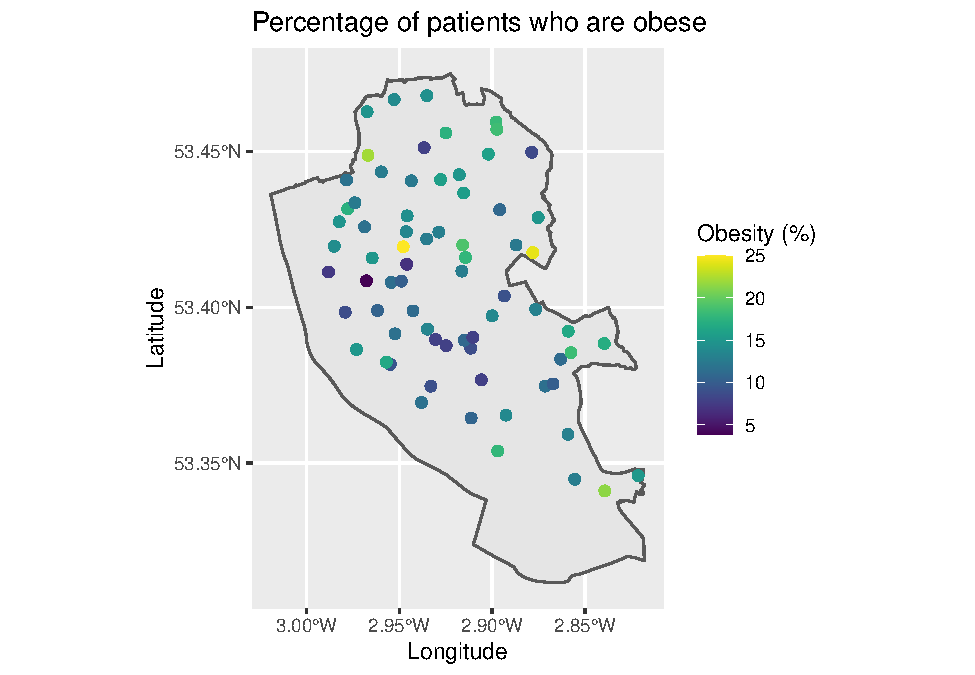
\includegraphics{Spatial-Data_files/figure-latex/unnamed-chunk-25-1.pdf}

This is a little hard to see general patterns, but follows what we learnt last week.

A second approach would be to adjust the size of the dots in relation to their value.

\begin{Shaded}
\begin{Highlighting}[]
\NormalTok{map5 }\OtherTok{\textless{}{-}} \FunctionTok{ggplot}\NormalTok{() }\SpecialCharTok{+} \CommentTok{\# Call ggplot2}
  \FunctionTok{geom\_sf}\NormalTok{(}\AttributeTok{data =}\NormalTok{ liverpool) }\SpecialCharTok{+} \CommentTok{\# Plot Liverpool outline}
  \FunctionTok{geom\_sf}\NormalTok{(}\AttributeTok{data =}\NormalTok{ gp\_locations\_sp, }\FunctionTok{aes}\NormalTok{(}\AttributeTok{size =}\NormalTok{ obese\_percent),) }\SpecialCharTok{+} \CommentTok{\# Define what to map}
  \FunctionTok{scale\_color\_viridis}\NormalTok{() }\SpecialCharTok{+} \CommentTok{\# Make colour blind friendly}
  \FunctionTok{xlab}\NormalTok{(}\StringTok{"Longitude"}\NormalTok{) }\SpecialCharTok{+} \CommentTok{\# Add x{-}axis label}
  \FunctionTok{ylab}\NormalTok{(}\StringTok{"Latitude"}\NormalTok{) }\SpecialCharTok{+} \CommentTok{\# Add y{-}axis label}
  \FunctionTok{labs}\NormalTok{(}\AttributeTok{title =} \StringTok{"Percentage of patients who are obese"}\NormalTok{, }\CommentTok{\# Edit plot title }
       \AttributeTok{size =} \StringTok{"Obesity (\%)"}\NormalTok{) }\CommentTok{\# Edit legend title (note must match size as that is what we are plotting)}
\NormalTok{map5}
\end{Highlighting}
\end{Shaded}

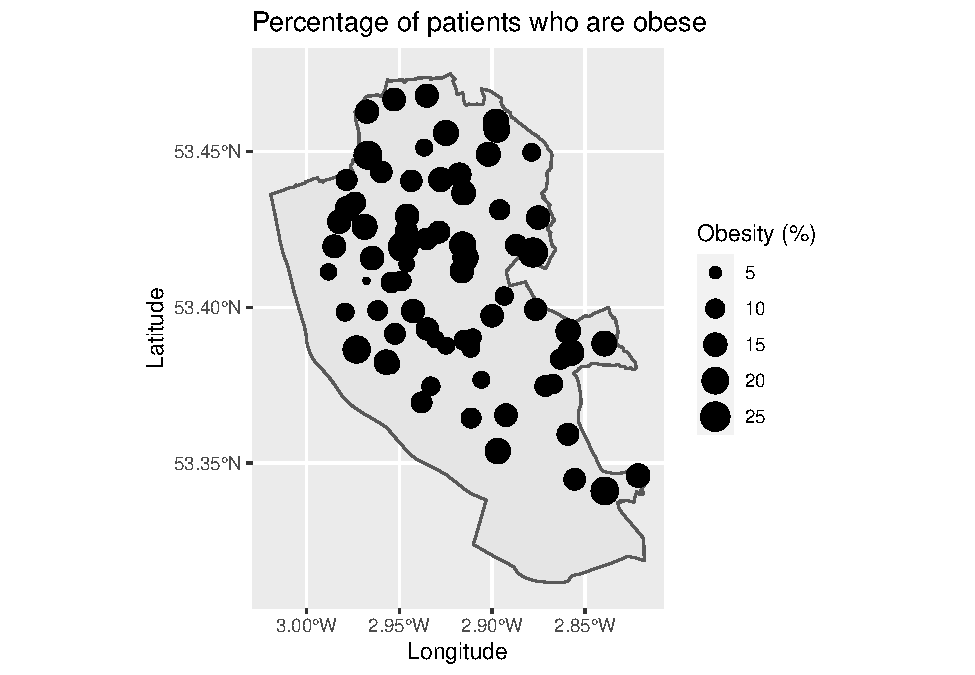
\includegraphics{Spatial-Data_files/figure-latex/unnamed-chunk-26-1.pdf}

Adjusting the size of points can be visually more striking, but is also harder to interpret the exact values. It is easier for the human mind to judge differences in colour rather than differences in sizes of points. Try identifying locations that are grouped as 15 or 20 on the map - it's hard!

Since our maps only present data for the spatial points themselves, we may want to estimate what the data might be like inbetween points to help identify the area extent of clusters or general spatial patterns. Here, we would turn to \textbf{spatial interpolation} techniques that can create a continuous surface based on given point values.

There are various spatial interpolation techniques that we can then use to fill in the gaps including inverse distance weighting or spatial kriging techniques. In this tutorial, we will just use non-linear \textbf{splines} to estimate values inbetween points. Splines are faster to run, but may give less precise results.

The following code below runs the interpolation code and then sorts the data out to a format for mapping. We need a couple of new packages here - \texttt{akima} and \texttt{reshape2} - although, we will only use them briefly so I will not describe them in detail.

\begin{Shaded}
\begin{Highlighting}[]
\CommentTok{\# Interpolate data}
\FunctionTok{library}\NormalTok{(akima) }\CommentTok{\# Load package}
\NormalTok{obese\_interp }\OtherTok{\textless{}{-}} \FunctionTok{with}\NormalTok{(gp\_locations, }\FunctionTok{interp}\NormalTok{(}\AttributeTok{x =}\NormalTok{ longitude, }\AttributeTok{y =}\NormalTok{ latitude, }\AttributeTok{z =}\NormalTok{ obese\_percent, }\AttributeTok{duplicate =} \StringTok{"mean"}\NormalTok{, }\AttributeTok{linear =} \ConstantTok{FALSE}\NormalTok{)) }\CommentTok{\# Set parameters for spatial location, what to predict, how to deal with duplicate values (i.e., take the mean), and linear = FALSE means uses cubic splines}

\CommentTok{\# Data wrangling}
\FunctionTok{library}\NormalTok{(reshape2) }\CommentTok{\# Load package}
\NormalTok{pred\_obese\_df }\OtherTok{\textless{}{-}} \FunctionTok{melt}\NormalTok{(obese\_interp}\SpecialCharTok{$}\NormalTok{z, }\AttributeTok{na.rm =} \ConstantTok{TRUE}\NormalTok{) }\CommentTok{\# Convert predicted values from a list (in wide format) to data frame (in long format)}
\FunctionTok{names}\NormalTok{(pred\_obese\_df) }\OtherTok{\textless{}{-}} \FunctionTok{c}\NormalTok{(}\StringTok{"x"}\NormalTok{, }\StringTok{"y"}\NormalTok{, }\StringTok{"obese\_percent"}\NormalTok{) }\CommentTok{\# Rename columns}

\CommentTok{\# Sort out longitude values}
\NormalTok{x }\OtherTok{\textless{}{-}} \FunctionTok{melt}\NormalTok{(obese\_interp}\SpecialCharTok{$}\NormalTok{x, }\AttributeTok{na.rm =} \ConstantTok{TRUE}\NormalTok{) }\CommentTok{\# Convert longitude values from list format to data frame}
\NormalTok{x }\OtherTok{\textless{}{-}} \FunctionTok{data.frame}\NormalTok{(}\FunctionTok{row.names}\NormalTok{(x), x, }\AttributeTok{row.names =} \ConstantTok{NULL}\NormalTok{) }\CommentTok{\# Save row values as column (these match up to melt values x)}
\FunctionTok{names}\NormalTok{(x) }\OtherTok{\textless{}{-}} \FunctionTok{c}\NormalTok{(}\StringTok{"x"}\NormalTok{, }\StringTok{"longitude"}\NormalTok{) }\CommentTok{\# Rename columns}
\NormalTok{pred\_obese\_df }\OtherTok{\textless{}{-}} \FunctionTok{merge}\NormalTok{(pred\_obese\_df, x, }\AttributeTok{by =} \StringTok{"x"}\NormalTok{, }\AttributeTok{all.x =}\NormalTok{ T) }\CommentTok{\# Join on longitude values to their lookup values from the melt process}
\FunctionTok{rm}\NormalTok{(x) }\CommentTok{\# Tidy}

\CommentTok{\# Sort out latitude values}
\NormalTok{y }\OtherTok{\textless{}{-}} \FunctionTok{melt}\NormalTok{(obese\_interp}\SpecialCharTok{$}\NormalTok{y, }\AttributeTok{na.rm =} \ConstantTok{TRUE}\NormalTok{) }\CommentTok{\# Convert longitude values from list format to data frame}
\NormalTok{y }\OtherTok{\textless{}{-}} \FunctionTok{data.frame}\NormalTok{(}\FunctionTok{row.names}\NormalTok{(y), y, }\AttributeTok{row.names =} \ConstantTok{NULL}\NormalTok{) }\CommentTok{\# Save row values as column (these match up to melt values y)}
\FunctionTok{names}\NormalTok{(y) }\OtherTok{\textless{}{-}} \FunctionTok{c}\NormalTok{(}\StringTok{"y"}\NormalTok{, }\StringTok{"latitude"}\NormalTok{) }\CommentTok{\# Rename columns}
\NormalTok{pred\_obese\_df }\OtherTok{\textless{}{-}} \FunctionTok{merge}\NormalTok{(pred\_obese\_df, y, }\AttributeTok{by =} \StringTok{"y"}\NormalTok{, }\AttributeTok{all.x =}\NormalTok{ T) }\CommentTok{\# Join on longitude values to their lookup values from the melt process}
\FunctionTok{rm}\NormalTok{(y) }\CommentTok{\# Tidy}
\end{Highlighting}
\end{Shaded}

Phew, that code was rather messy but it does get the job done (if you know a better way, let me know!). We can now plot it using a heat map.

\begin{Shaded}
\begin{Highlighting}[]
\NormalTok{map6 }\OtherTok{\textless{}{-}} \FunctionTok{ggplot}\NormalTok{() }\SpecialCharTok{+} \CommentTok{\# Call ggplot2}
  \FunctionTok{geom\_sf}\NormalTok{(}\AttributeTok{data =}\NormalTok{ liverpool) }\SpecialCharTok{+} \CommentTok{\# Plot Liverpool outline}
  \FunctionTok{geom\_tile}\NormalTok{(}\AttributeTok{data =}\NormalTok{ pred\_obese\_df, }\FunctionTok{aes}\NormalTok{(}\AttributeTok{x =}\NormalTok{ longitude, }\AttributeTok{y =}\NormalTok{ latitude, }\AttributeTok{fill =}\NormalTok{ obese\_percent)) }\SpecialCharTok{+} \CommentTok{\# Define what to map (interpolated values)}
  \FunctionTok{scale\_fill\_viridis}\NormalTok{() }\SpecialCharTok{+} \CommentTok{\# Make colour blind friendly}
  \FunctionTok{xlab}\NormalTok{(}\StringTok{"Longitude"}\NormalTok{) }\SpecialCharTok{+} \CommentTok{\# Add x{-}axis label}
  \FunctionTok{ylab}\NormalTok{(}\StringTok{"Latitude"}\NormalTok{) }\SpecialCharTok{+} \CommentTok{\# Add y{-}axis label}
  \FunctionTok{labs}\NormalTok{(}\AttributeTok{title =} \StringTok{"Estimated obesity prevalence"}\NormalTok{, }\CommentTok{\# Edit plot title }
       \AttributeTok{fill =} \StringTok{"Obesity (\%)"}\NormalTok{) }\CommentTok{\# Edit legend title (note must match fill as that is what we are plotting)}
\NormalTok{map6}
\end{Highlighting}
\end{Shaded}

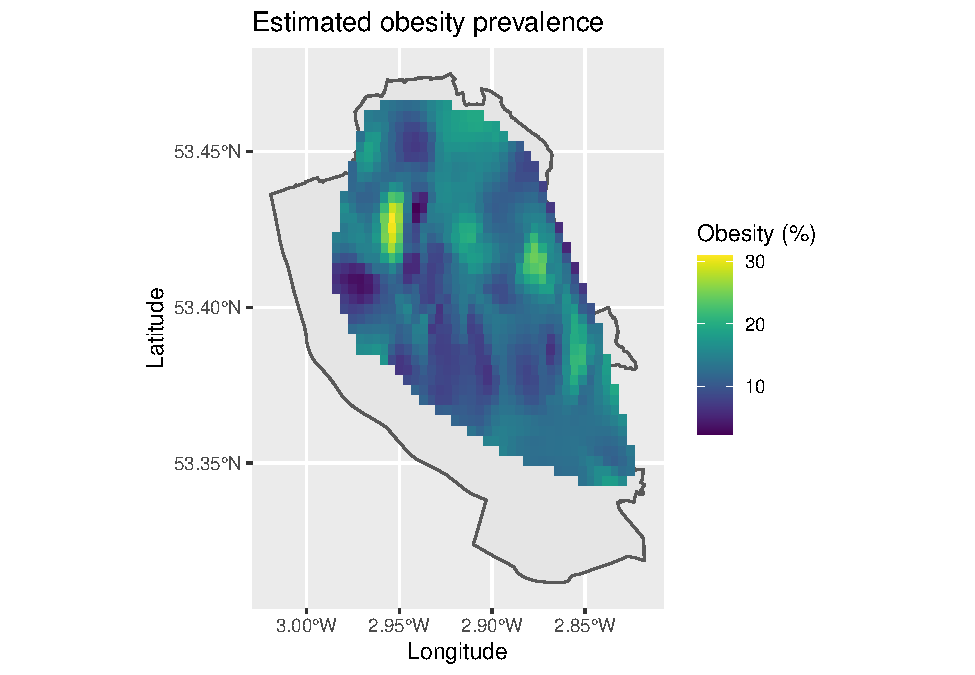
\includegraphics{Spatial-Data_files/figure-latex/unnamed-chunk-28-1.pdf}

We should be careful in producing these maps, since we are estimating data inbetween points and the resulting maps may not be correct. For example, it makes an assumption that people go to their nearest GP surgery to where they live, which is not always true. We can see a cluster of high levels of obesity north of the city centre, which is a densely populated deprived area. However, there is a lot of variability in the data and it is a little messy. Hopefully at least it gives you can idea of how to use these techniques and what they can produce.

Can you produce a similar map for chronic health disease prevalence? (tip: the variable required is \texttt{gp\_locations\$chronic\_heart\_disease\_percent}).

\hypertarget{area-data}{%
\section{Area data}\label{area-data}}

These techniques introduced for point-based data do not work with area data. However, we can utilise more powerful techniques to examine the existence of clustering in our data.

We will utilise a new R package - \texttt{spdep} (Spatial Dependence). The package includes a range of functions that are useful for creating spatial weighting schemes which are useful for identifying the spatial structure of datasets, as well as some spatial analysis methods including the spatial autocorrelation measures we will use here.

To highlight some of these techniques, we will return to the data on vaccination uptake from the previous tutorial. Let's load in the data and remind ourselves of the spatial patterns it contained.

\begin{Shaded}
\begin{Highlighting}[]
\CommentTok{\# Get data ready}
\NormalTok{msoas }\OtherTok{\textless{}{-}} \FunctionTok{read\_sf}\NormalTok{(}\StringTok{"./Shapefiles/Liverpool\_MSOAs/england\_msoa\_2011.shp"}\NormalTok{)  }\CommentTok{\# Load in shapefile for Liverpool MSOAs}
\NormalTok{vaccine\_uptake }\OtherTok{\textless{}{-}} \FunctionTok{read.csv}\NormalTok{(}\StringTok{"./Data/msoa\_vaccine\_10June21.csv"}\NormalTok{) }\CommentTok{\# Load in vaccine uptake data}
\NormalTok{msoas }\OtherTok{\textless{}{-}} \FunctionTok{merge}\NormalTok{(msoas, vaccine\_uptake, }\AttributeTok{by.x =} \StringTok{"code"}\NormalTok{, }\AttributeTok{by.y =} \StringTok{"msoa\_code"}\NormalTok{, }\AttributeTok{all.x =} \ConstantTok{TRUE}\NormalTok{) }\CommentTok{\# Merge the vaccine uptake objects onto the msoa object, based on the columns defined (x = msoas, y = vaccine\_uptake), and do this for all observations only in the x (msoas) object}

\CommentTok{\# Map}
\NormalTok{map7 }\OtherTok{\textless{}{-}} \FunctionTok{ggplot}\NormalTok{() }\SpecialCharTok{+} \CommentTok{\# Call ggplot command}
            \FunctionTok{geom\_sf}\NormalTok{(}\AttributeTok{data =}\NormalTok{ msoas, }\FunctionTok{aes}\NormalTok{(}\AttributeTok{fill =}\NormalTok{ total\_first\_dose), }\AttributeTok{lwd =} \DecValTok{0}\NormalTok{) }\SpecialCharTok{+} \CommentTok{\# Using a spatial object, plot MSOAs and fill in based on number of people with first COVID{-}19 dose, with line width = 0 (i.e., not visible)}
            \FunctionTok{scale\_fill\_viridis\_c}\NormalTok{(}\AttributeTok{option =} \StringTok{"plasma"}\NormalTok{) }\SpecialCharTok{+} \CommentTok{\# Make colour{-}blind friendly}
            \FunctionTok{xlab}\NormalTok{(}\StringTok{"Longitude"}\NormalTok{) }\SpecialCharTok{+} \CommentTok{\# Add x{-}axis label}
            \FunctionTok{ylab}\NormalTok{(}\StringTok{"Latitude"}\NormalTok{) }\SpecialCharTok{+} \CommentTok{\# Add y{-}axis label}
            \FunctionTok{labs}\NormalTok{(}\AttributeTok{title =} \StringTok{"First dose COVID{-}19 vaccinations"}\NormalTok{, }\CommentTok{\# Add title to map}
                 \AttributeTok{fill =} \StringTok{"Frequency"}\NormalTok{) }\CommentTok{\# Edit legend title}
\NormalTok{map7 }\CommentTok{\# Print plot}
\end{Highlighting}
\end{Shaded}

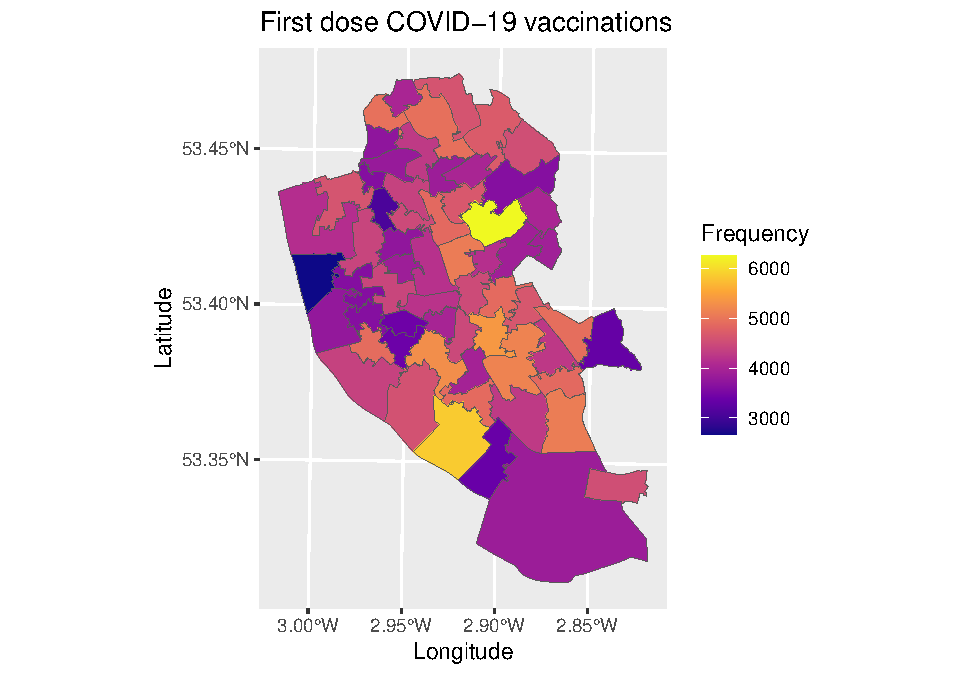
\includegraphics{Spatial-Data_files/figure-latex/unnamed-chunk-29-1.pdf}

\hypertarget{global-morans-i}{%
\subsection{Global Moran's I}\label{global-morans-i}}

The first step we would want to take is to describe the overall extent of spatial clustering of any variable. To do this, we will calculate a global Moran's I statistic that can tell us the extent of clustering of data. You can review the methodology behind this in the related lecture slides \href{}{here}.

To be able to describe the clustering, we need to tell R about the spatial structure of our dataset. Specifically, we need to identify which areas are located next to each other (i.e., neighbours).

As we are dealing with area (polygons) spatial data, we will define spatial neighbours based on which borders they match on. So if two areas share a common border, then we can define them as neighbouring each other. There are two ways of defining this process:

\begin{itemize}
\tightlist
\item
  Rook contiguity - only areas that share common borders/edges of some defined length
\item
  Queen contiguity - all areas that touch each other are considered neighbours, even if the shared space is very small
\end{itemize}

To calculate the spatial structuring of neighbouring areas, we run the following code.

\begin{Shaded}
\begin{Highlighting}[]
\FunctionTok{library}\NormalTok{(spdep) }\CommentTok{\# Load package}
\end{Highlighting}
\end{Shaded}

\begin{verbatim}
## Loading required package: sp
\end{verbatim}

\begin{verbatim}
## Loading required package: spData
\end{verbatim}

\begin{verbatim}
## To access larger datasets in this package, install the spDataLarge package with:
## `install.packages('spDataLarge', repos='https://nowosad.github.io/drat/', type='source')`
\end{verbatim}

\begin{Shaded}
\begin{Highlighting}[]
\NormalTok{nb }\OtherTok{\textless{}{-}} \FunctionTok{poly2nb}\NormalTok{(msoas, }\AttributeTok{queen =} \ConstantTok{TRUE}\NormalTok{) }\CommentTok{\# Calculate queen contiguity for areas (set queen = FALSE for rook contiguity)}
\end{Highlighting}
\end{Shaded}

We now need to assign spatial weights to each area (polygon) based on the spatial structure of the data. These weights are important when we are calculating the average values of neighbours, but adjusting their values.

\begin{Shaded}
\begin{Highlighting}[]
\NormalTok{lw }\OtherTok{\textless{}{-}} \FunctionTok{nb2listw}\NormalTok{(nb, }\AttributeTok{style =} \StringTok{"W"}\NormalTok{, }\AttributeTok{zero.policy =} \ConstantTok{TRUE}\NormalTok{) }\CommentTok{\# Assign weights based on list of neighbours. Each neighbouring area is given an equal weighting (syle = "W"). Zero.policy = TRUE allows for areas with no neighbours.}
\end{Highlighting}
\end{Shaded}

Now that we have weightings for each areas linked to its neighbours, we can calculate the global Moran's I. Essentially, it is looking at the correlation between each area's value and the average values for surrounding neighbours. This gives a crude descriptive value of the amount of clustering in our data - it is termed `global' since it is an average for all areas.

\begin{Shaded}
\begin{Highlighting}[]
\NormalTok{m1 }\OtherTok{\textless{}{-}} \FunctionTok{moran.test}\NormalTok{(msoas}\SpecialCharTok{$}\NormalTok{total\_first\_dose, lw) }\CommentTok{\# Calculate Moran\textquotesingle{}s I}
\NormalTok{m1 }\CommentTok{\# Print result}
\end{Highlighting}
\end{Shaded}

\begin{verbatim}
## 
##  Moran I test under randomisation
## 
## data:  msoas$total_first_dose  
## weights: lw    
## 
## Moran I statistic standard deviate = 1.5264, p-value = 0.06345
## alternative hypothesis: greater
## sample estimates:
## Moran I statistic       Expectation          Variance 
##       0.107062246      -0.016666667       0.006570535
\end{verbatim}

There is a lot of output here, however we are really only interested in two things mostly. The Moran's I statistic is 0.1070622. We interpret the estimated value was running between -1 and 1, where values closer to 1 suggest existence of spatial clustering, values of 0 suggesting no clustering (i.e., random), and values less than 0 suggesting evenly dispersed values (rare in the real world). Some rules of thumbs - a value of 0.3 would suggest low-moderate clustering, with values 0.5+ suggestung moderate to high clustering. A value of 0.1070622 suggests little evidence of clustering in the data.

We can also consider the p-value to assess if the result is statistically significant \sout{notwithstanding the continued controversy on using p-values}. A value of 0.0634541 suggests that the result is not statistically significant, lending further evidence towards a conclusion that there is little evidence of spatial clustering.

To get a more accurate p-value, we should use Monte Carlo simulations to estimate it. Let's try this, but this time looking at the clustering of second dose COVID-19 vaccinations.

\begin{Shaded}
\begin{Highlighting}[]
\NormalTok{m2 }\OtherTok{\textless{}{-}} \FunctionTok{moran.mc}\NormalTok{(msoas}\SpecialCharTok{$}\NormalTok{total\_second\_dose, lw, }\AttributeTok{nsim =} \DecValTok{1000}\NormalTok{) }\CommentTok{\# Calculate Moran\textquotesingle{}s I and simulate 1000 times permutations to give more accurate p{-}value}
\NormalTok{m2 }\CommentTok{\# Print result}
\end{Highlighting}
\end{Shaded}

\begin{verbatim}
## 
##  Monte-Carlo simulation of Moran I
## 
## data:  msoas$total_second_dose 
## weights: lw  
## number of simulations + 1: 1001 
## 
## statistic = 0.30176, observed rank = 1001, p-value = 0.000999
## alternative hypothesis: greater
\end{verbatim}

Here we find some evidence of clustering in the data, with a value of suggesting low to moderate clustering in the data.

\begin{Shaded}
\begin{Highlighting}[]
\NormalTok{m2\_plot }\OtherTok{\textless{}{-}} \FunctionTok{moran.plot}\NormalTok{(msoas}\SpecialCharTok{$}\NormalTok{total\_second\_dose, }\AttributeTok{listw =}\NormalTok{ lw, }\AttributeTok{plot =} \ConstantTok{FALSE}\NormalTok{)  }\CommentTok{\# Save raw moran\textquotesingle{}s I data (if run without saving as an object, it will plot in base R if you set plot = TRUE (default){-} for our purposes, I have shown how to get it into ggplot2 as it looks nicer}

\CommentTok{\# Plot}
\NormalTok{plot1 }\OtherTok{\textless{}{-}} \FunctionTok{ggplot}\NormalTok{(}\AttributeTok{data =}\NormalTok{ m2\_plot, }\FunctionTok{aes}\NormalTok{(}\AttributeTok{x =}\NormalTok{ x, }\AttributeTok{y =}\NormalTok{ wx)) }\SpecialCharTok{+} \CommentTok{\# Plot x (actual values) and wx (average for neighbours)}
    \FunctionTok{geom\_point}\NormalTok{() }\SpecialCharTok{+} \CommentTok{\# Scatter plot}
    \FunctionTok{geom\_smooth}\NormalTok{(}\AttributeTok{method =} \StringTok{"lm"}\NormalTok{) }\SpecialCharTok{+} \CommentTok{\# Line of best fit}
    \FunctionTok{xlab}\NormalTok{(}\StringTok{"Number of second doses"}\NormalTok{) }\SpecialCharTok{+} \CommentTok{\# Label x{-}axis}
    \FunctionTok{ylab}\NormalTok{(}\StringTok{"Spatially lagged number of second doses"}\NormalTok{)}
\NormalTok{plot1 }\CommentTok{\# Print plot}
\end{Highlighting}
\end{Shaded}

\begin{verbatim}
## `geom_smooth()` using formula 'y ~ x'
\end{verbatim}

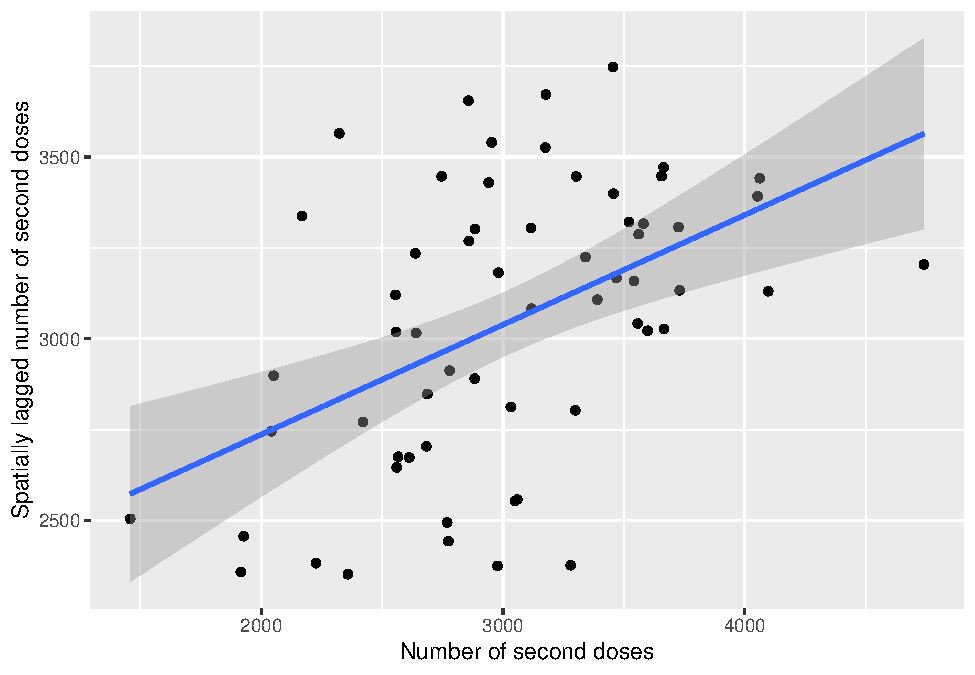
\includegraphics{Spatial-Data_files/figure-latex/unnamed-chunk-34-1.pdf}

\hypertarget{local-morans-i}{%
\subsection{Local Moran's I}\label{local-morans-i}}

If we find evidence of clustering overall, then the next step is to describe where this clustering exists. The global Moran's I for number of second COVID-19 vaccine doses suggested some clustering of values, let's explore where the clustering exists and the nature of it. Using a local Moran's I, we can calculate the extent each area belongs to a cluster of high or low values.

\begin{Shaded}
\begin{Highlighting}[]
\CommentTok{\# Estimate metrics}
\NormalTok{local\_2nd }\OtherTok{\textless{}{-}} \FunctionTok{localmoran}\NormalTok{(}\AttributeTok{x =}\NormalTok{ msoas}\SpecialCharTok{$}\NormalTok{total\_second\_dose, }\AttributeTok{listw =}\NormalTok{ lw) }\CommentTok{\# Calculate local Moran\textquotesingle{}s I}
\CommentTok{\# local\_2nd \textless{}{-} localmoran\_perm((x = msoas$total\_second\_dose, listw = lw, nsim=499) \# In case want to run more simulations to get a more accurate level of significance}
\NormalTok{local\_2nd\_map }\OtherTok{\textless{}{-}} \FunctionTok{cbind}\NormalTok{(msoas, local\_2nd) }\CommentTok{\# Join estimates onto shapefile for MSOAs}

\CommentTok{\# Map}
\NormalTok{map8 }\OtherTok{\textless{}{-}} \FunctionTok{ggplot}\NormalTok{() }\SpecialCharTok{+}
  \FunctionTok{geom\_sf}\NormalTok{(}\AttributeTok{data =}\NormalTok{ local\_2nd\_map, }\FunctionTok{aes}\NormalTok{(}\AttributeTok{fill =}\NormalTok{ Ii)) }\SpecialCharTok{+} \CommentTok{\# Plot local Moran\textquotesingle{}s I statistic (z score)}
  \FunctionTok{scale\_fill\_viridis}\NormalTok{() }\SpecialCharTok{+} \CommentTok{\# Make colour blind friendly}
  \FunctionTok{xlab}\NormalTok{(}\StringTok{"Longitude"}\NormalTok{) }\SpecialCharTok{+} \CommentTok{\# Add x{-}axis label}
  \FunctionTok{ylab}\NormalTok{(}\StringTok{"Latitude"}\NormalTok{) }\SpecialCharTok{+} \CommentTok{\# Add y{-}axis label}
  \FunctionTok{labs}\NormalTok{(}\AttributeTok{title =} \StringTok{"Clustering of second dose uptake"}\NormalTok{, }\CommentTok{\# Edit plot title }
       \AttributeTok{fill =} \StringTok{"Local Moran\textquotesingle{}s I"}\NormalTok{) }\CommentTok{\# Edit legend title (note must match fill as that is what we are plotting)}
\NormalTok{map8 }\CommentTok{\# Plot}
\end{Highlighting}
\end{Shaded}

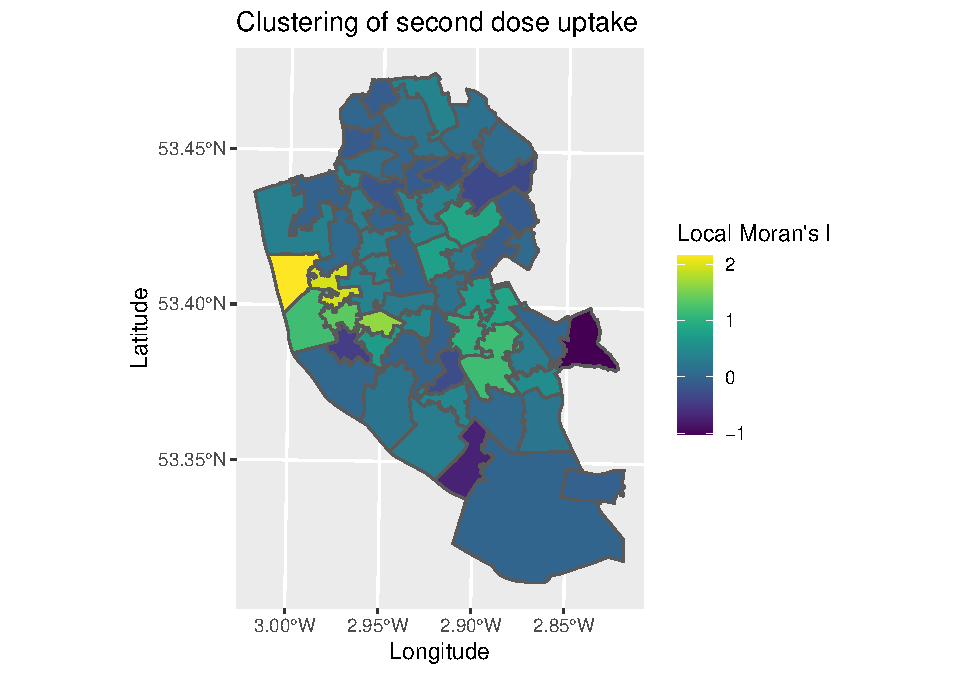
\includegraphics{Spatial-Data_files/figure-latex/unnamed-chunk-35-1.pdf}

The map tells us how different each area is to it's surrounding areas , with areas with higher z-scores representing areas that are clustered by higher values in the surrounding areas, and lower scores the opposite (surrounded by lower values). The map suggests a cluster in the city centre area, as well as a less distinct one to the South East. To understand how meaningful these spatial patterns are, we can plot the p-values for areas.

\begin{Shaded}
\begin{Highlighting}[]
\NormalTok{map9 }\OtherTok{\textless{}{-}} \FunctionTok{ggplot}\NormalTok{() }\SpecialCharTok{+}
  \FunctionTok{geom\_sf}\NormalTok{(}\AttributeTok{data =}\NormalTok{ local\_2nd\_map, }\FunctionTok{aes}\NormalTok{(}\AttributeTok{fill =}\NormalTok{ Pr.z...}\FloatTok{0.}\NormalTok{)) }\SpecialCharTok{+} \CommentTok{\# Plot local Moran\textquotesingle{}s I statistic (z score)}
  \FunctionTok{scale\_fill\_viridis}\NormalTok{() }\SpecialCharTok{+} \CommentTok{\# Make colour blind friendly}
  \FunctionTok{xlab}\NormalTok{(}\StringTok{"Longitude"}\NormalTok{) }\SpecialCharTok{+} \CommentTok{\# Add x{-}axis label}
  \FunctionTok{ylab}\NormalTok{(}\StringTok{"Latitude"}\NormalTok{) }\SpecialCharTok{+} \CommentTok{\# Add y{-}axis label}
  \FunctionTok{labs}\NormalTok{(}\AttributeTok{title =} \StringTok{"Clustering of second dose uptake"}\NormalTok{, }\CommentTok{\# Edit plot title }
       \AttributeTok{fill =} \StringTok{"p{-}value"}\NormalTok{) }\CommentTok{\# Edit legend title (note must match fill as that is what we are plotting)}
\NormalTok{map9 }\CommentTok{\# Plot}
\end{Highlighting}
\end{Shaded}

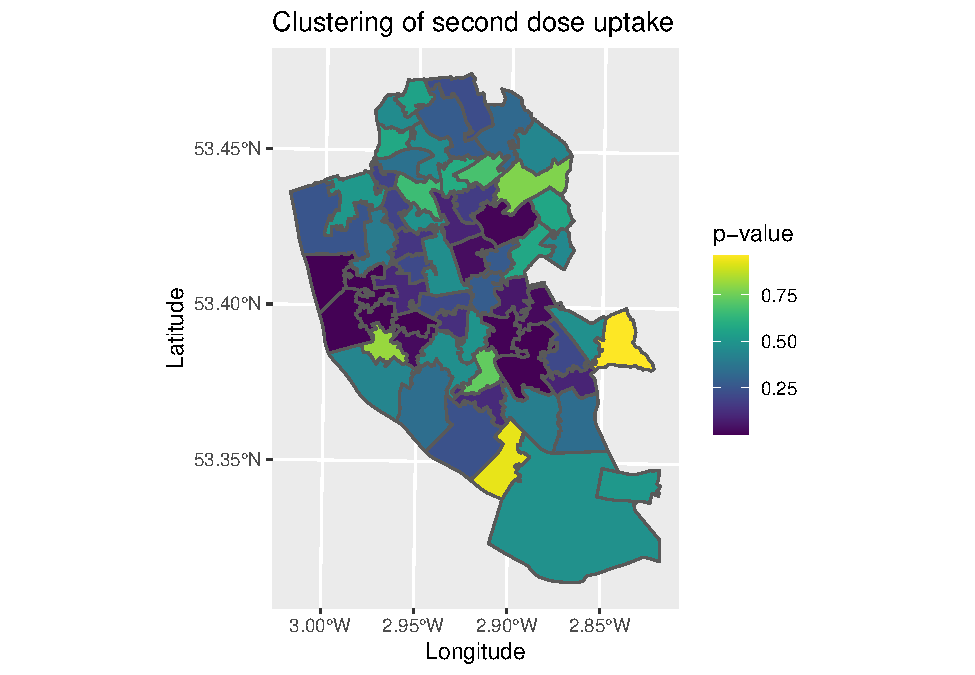
\includegraphics{Spatial-Data_files/figure-latex/unnamed-chunk-36-1.pdf}

What the map is missing is the nature of the clusters. We can say with some confidence that there is a cluster in the city centre for example, but we are not sure what this is a cluster of. We could compare manually to \texttt{map7}, however it would be useful to have a single map the brings together all of this information. To help contextualise the clustering analysis, we need to classify the local Moran's I data to describe their patterns.

\begin{Shaded}
\begin{Highlighting}[]
\CommentTok{\# Data wrangling}
\NormalTok{quadrant }\OtherTok{\textless{}{-}} \FunctionTok{vector}\NormalTok{(}\AttributeTok{mode=}\StringTok{"numeric"}\NormalTok{, }\AttributeTok{length =} \FunctionTok{nrow}\NormalTok{(local\_2nd)) }\CommentTok{\# Create blank object for storing results}
\NormalTok{m\_2nd }\OtherTok{\textless{}{-}}\NormalTok{ msoas}\SpecialCharTok{$}\NormalTok{total\_second\_dose }\SpecialCharTok{{-}} \FunctionTok{mean}\NormalTok{(msoas}\SpecialCharTok{$}\NormalTok{total\_second\_dose) }\CommentTok{\# Centers each area around its mean (for variable under investigation)}
\NormalTok{m\_localmi }\OtherTok{\textless{}{-}}\NormalTok{ local\_2nd[,}\DecValTok{1}\NormalTok{] }\SpecialCharTok{{-}} \FunctionTok{mean}\NormalTok{(local\_2nd[,}\DecValTok{1}\NormalTok{]) }\CommentTok{\# Centers areas on the local Moran\textquotesingle{}s I values around the mean}
\NormalTok{sig }\OtherTok{\textless{}{-}} \FloatTok{0.1} \CommentTok{\# Define statistical significance threshold (feel free to select more stringent values)}

\CommentTok{\# Populate the blank object with our classification of results}
\NormalTok{quadrant[m\_2nd }\SpecialCharTok{\textless{}} \DecValTok{0} \SpecialCharTok{\&}\NormalTok{ m\_localmi }\SpecialCharTok{\textless{}} \DecValTok{0}\NormalTok{] }\OtherTok{\textless{}{-}} \DecValTok{1} \CommentTok{\# Low{-}low: Lower than average raw value, lower than average surrounding areas}
\NormalTok{quadrant[m\_2nd }\SpecialCharTok{\textless{}} \DecValTok{0} \SpecialCharTok{\&}\NormalTok{ m\_localmi }\SpecialCharTok{\textgreater{}} \DecValTok{0}\NormalTok{] }\OtherTok{\textless{}{-}} \DecValTok{2} \CommentTok{\# Low{-}high: Lower than average raw value, higher than average surrounding areas}
\NormalTok{quadrant[m\_2nd }\SpecialCharTok{\textgreater{}} \DecValTok{0} \SpecialCharTok{\&}\NormalTok{ m\_localmi }\SpecialCharTok{\textless{}} \DecValTok{0}\NormalTok{] }\OtherTok{\textless{}{-}} \DecValTok{3} \CommentTok{\# High{-}low: Higher than average raw value, lower than average surrounding areas}
\NormalTok{quadrant[m\_2nd }\SpecialCharTok{\textgreater{}} \DecValTok{0} \SpecialCharTok{\&}\NormalTok{ m\_localmi }\SpecialCharTok{\textgreater{}} \DecValTok{0}\NormalTok{] }\OtherTok{\textless{}{-}} \DecValTok{4} \CommentTok{\# High{-}high: Higher than average raw value, higher than average surrounding areas}
\NormalTok{quadrant[local\_2nd[,}\DecValTok{5}\NormalTok{] }\SpecialCharTok{\textgreater{}}\NormalTok{ sig] }\OtherTok{\textless{}{-}} \DecValTok{0} \CommentTok{\# Identify non{-}significant areas}
\NormalTok{quadrant }\OtherTok{\textless{}{-}} \FunctionTok{factor}\NormalTok{(quadrant, }\AttributeTok{levels =} \FunctionTok{c}\NormalTok{(}\StringTok{"0"}\NormalTok{, }\StringTok{"1"}\NormalTok{, }\StringTok{"2"}\NormalTok{, }\StringTok{"3"}\NormalTok{, }\StringTok{"4"}\NormalTok{)) }\CommentTok{\# Define variable as factor (as distinct categories)}
\NormalTok{local\_2nd\_map2 }\OtherTok{\textless{}{-}} \FunctionTok{cbind}\NormalTok{(msoas, quadrant) }\CommentTok{\# Join data onto the original shapefile}

\CommentTok{\# Plot}
\NormalTok{map10 }\OtherTok{\textless{}{-}} \FunctionTok{ggplot}\NormalTok{() }\SpecialCharTok{+}
  \FunctionTok{geom\_sf}\NormalTok{(}\AttributeTok{data =}\NormalTok{ local\_2nd\_map2, }\FunctionTok{aes}\NormalTok{(}\AttributeTok{fill =}\NormalTok{ quadrant)) }\SpecialCharTok{+} \CommentTok{\# Plot values}
  \FunctionTok{scale\_fill\_manual}\NormalTok{(}\AttributeTok{values =} \FunctionTok{c}\NormalTok{(}\StringTok{"0"} \OtherTok{=} \StringTok{"white"}\NormalTok{, }\StringTok{"1"} \OtherTok{=} \StringTok{"blue"}\NormalTok{, }\StringTok{"2"} \OtherTok{=} \FunctionTok{rgb}\NormalTok{(}\DecValTok{0}\NormalTok{,}\DecValTok{0}\NormalTok{,}\DecValTok{1}\NormalTok{,}\AttributeTok{alpha=}\FloatTok{0.4}\NormalTok{), }\StringTok{"3"} \OtherTok{=} \FunctionTok{rgb}\NormalTok{(}\DecValTok{1}\NormalTok{,}\DecValTok{0}\NormalTok{,}\DecValTok{0}\NormalTok{,}\AttributeTok{alpha=}\FloatTok{0.4}\NormalTok{), }\StringTok{"4"} \OtherTok{=} \StringTok{"red"}\NormalTok{),}
                    \AttributeTok{labels =} \FunctionTok{c}\NormalTok{(}\StringTok{"Insignificant"}\NormalTok{, }\StringTok{"Low{-}low"}\NormalTok{, }\StringTok{"Low{-}high"}\NormalTok{, }\StringTok{"High{-}low"}\NormalTok{, }\StringTok{"High{-}high"}\NormalTok{),}
                    \AttributeTok{breaks =} \FunctionTok{c}\NormalTok{(}\DecValTok{0}\NormalTok{, }\DecValTok{1}\NormalTok{, }\DecValTok{2}\NormalTok{, }\DecValTok{3}\NormalTok{, }\DecValTok{4}\NormalTok{), }
                    \AttributeTok{drop =} \ConstantTok{FALSE}\NormalTok{) }\SpecialCharTok{+} \CommentTok{\# Show all values in legend}
  \FunctionTok{labs}\NormalTok{(}\AttributeTok{title =} \StringTok{"Clustering of second dose uptake"}\NormalTok{, }\CommentTok{\# Edit plot title }
    \AttributeTok{fill =} \StringTok{"Clusters"}\NormalTok{) }\SpecialCharTok{+} \CommentTok{\# Edit legend title (note must match fill as that is what we are plotting)}
  \FunctionTok{xlab}\NormalTok{(}\StringTok{"Longitude"}\NormalTok{) }\SpecialCharTok{+} \CommentTok{\# Add labels}
  \FunctionTok{ylab}\NormalTok{(}\StringTok{"Latitude"}\NormalTok{)}
\NormalTok{map10 }\CommentTok{\# Print}
\end{Highlighting}
\end{Shaded}

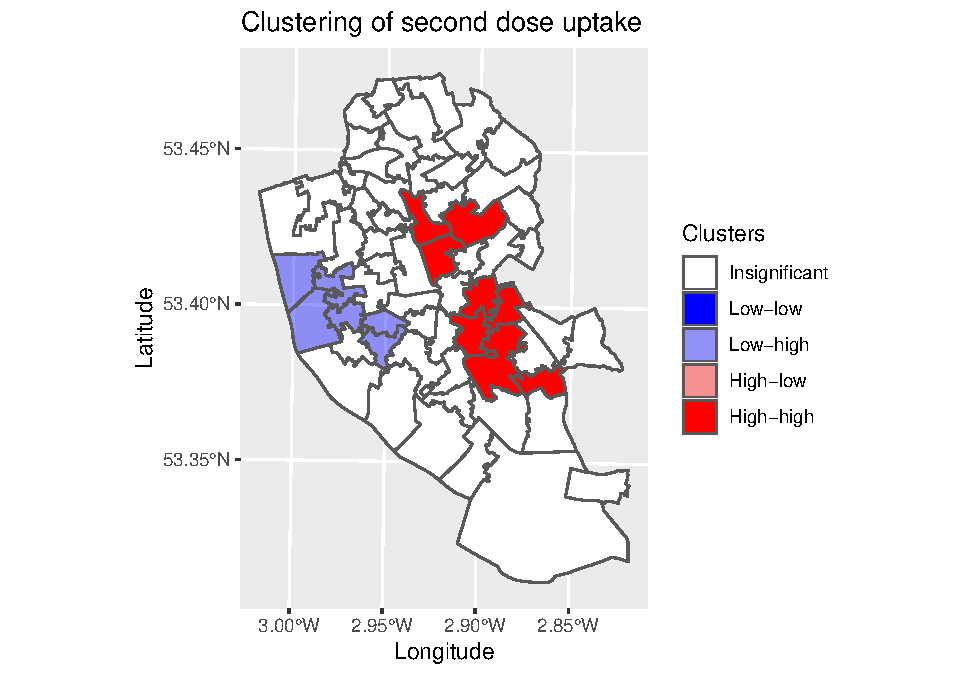
\includegraphics{Spatial-Data_files/figure-latex/unnamed-chunk-37-1.pdf}

This map is a common output in local Moran's I analyses. It combines the raw data, clustering analysis and associated statistical significance into a single plot. We can see that in the city centre, we have a cluster of low vaccination uptake surrounded by areas with higher values. We then have two significant clusters to the East, representing clusters of higher uptake.

\hypertarget{getis-ord-gi-statistic}{%
\subsection{Getis-Ord Gi statistic}\label{getis-ord-gi-statistic}}

An alternative clustering metric is the Getis-Ord Gi statistic. The Gi statistic is presented as a z-score, with positive values representing clusters of high values and negative values representing clusters of low values.

We can calculate the Gi statistic using the following code.

\begin{Shaded}
\begin{Highlighting}[]
\NormalTok{localGi }\OtherTok{\textless{}{-}} \FunctionTok{localG}\NormalTok{(msoas}\SpecialCharTok{$}\NormalTok{total\_second\_dose, }\AttributeTok{listw =}\NormalTok{ lw) }\CommentTok{\# Calculate Gi statistics for each MSOA (second dose total)}
\end{Highlighting}
\end{Shaded}

As before, the power of the clustering metrics is seen when we map it. Let's visualise the spatial pattern of clustering.

\begin{Shaded}
\begin{Highlighting}[]
\CommentTok{\# Wrangle data}
\NormalTok{Gi\_map }\OtherTok{\textless{}{-}} \FunctionTok{cbind}\NormalTok{(msoas, }\FunctionTok{data.matrix}\NormalTok{(localGi)) }\CommentTok{\# Join results onto shapefile}
\FunctionTok{names}\NormalTok{(Gi\_map)[}\FunctionTok{names}\NormalTok{(Gi\_map) }\SpecialCharTok{==} \StringTok{"data.matrix.localGi."}\NormalTok{] }\OtherTok{\textless{}{-}} \StringTok{"gstat"} \CommentTok{\# Rename column}

\CommentTok{\# Map}
\NormalTok{map11 }\OtherTok{\textless{}{-}} \FunctionTok{ggplot}\NormalTok{() }\SpecialCharTok{+}
  \FunctionTok{geom\_sf}\NormalTok{(}\AttributeTok{data =}\NormalTok{ Gi\_map, }\FunctionTok{aes}\NormalTok{(}\AttributeTok{fill =}\NormalTok{ gstat)) }\SpecialCharTok{+}
  \FunctionTok{scale\_fill\_viridis}\NormalTok{() }\SpecialCharTok{+} \CommentTok{\# Make colour blind friendly}
  \FunctionTok{xlab}\NormalTok{(}\StringTok{"Longitude"}\NormalTok{) }\SpecialCharTok{+} \CommentTok{\# Add x{-}axis label}
  \FunctionTok{ylab}\NormalTok{(}\StringTok{"Latitude"}\NormalTok{) }\SpecialCharTok{+} \CommentTok{\# Add y{-}axis label}
  \FunctionTok{labs}\NormalTok{(}\AttributeTok{title =} \StringTok{"Second dose uptake"}\NormalTok{, }\CommentTok{\# Edit plot title }
       \AttributeTok{fill =} \StringTok{"Gi statistic"}\NormalTok{) }\CommentTok{\# Edit legend title (note must match fill as that is what we are plotting)}
\NormalTok{map11}
\end{Highlighting}
\end{Shaded}

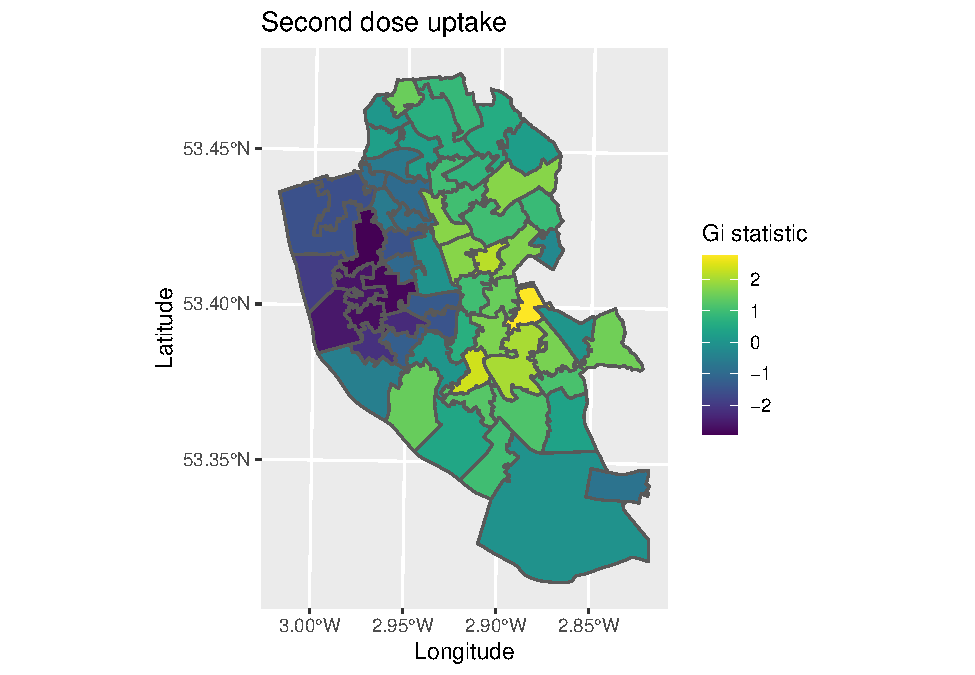
\includegraphics{Spatial-Data_files/figure-latex/unnamed-chunk-39-1.pdf}

The map produced is both similar and different to the local Moran's I. We see clustering in the city centre (younger populations) and north parts of Liverpool (more deprived communities), with higher vaccinate uptake in the more affluent South and South-East parts of the city.

\hypertarget{summary-1}{%
\section{Summary}\label{summary-1}}

So far, you have learned how to use spatial data in R, visualise and map their patterns, and start to analyse the spatial patterns themselves. Next we will move onto spatial extensions of regression techniques.

\hypertarget{spatreg}{%
\chapter{Spatial Regression}\label{spatreg}}

So far we have learned how to visualise spatial data and explore if patterns display clustering of high/low values. However, what if we want to understand the predictors of spatial patterns? In this section, we extend regression techniques to incorporate the spatial structure of data. The lecture slides for this practical can be found \href{}{here}. A PDF version of the practical can be found \href{}{here}.

\hypertarget{exploring-the-data}{%
\section{Exploring the data}\label{exploring-the-data}}

In this tutorial, we will focus on understanding geographical patterns in COVID-19 vaccination uptake. Our analysis will use data collected for Local Authorities Districts (LADs). LADs are large administrative areas that correspond to Local Government areas, typically equivalent to a city, large town or region.

I have collected data on uptake of COVID-19 vaccines (split by number of first and second doses upto 17th June 2021 from \href{https://www.england.nhs.uk/statistics/statistical-work-areas/covid-19-vaccinations/}{here}. We will focus on the percentage of people who have had their first vaccination dose as our outcome variable of interest here. I have also compiled a suite of explanatory and contextual variables to help understand patterns in vaccination uptake. These include:

\begin{itemize}
\tightlist
\item
  \textbf{Population} data was gathered to provde the denominator for our outcome variables. These data are for mid-year 2019 (\textasciitilde July) and were the most recent available statistics available at the time. Data were downloaded from \href{https://www.ons.gov.uk/peoplepopulationandcommunity/populationandmigration/populationestimates/datasets/populationestimatesforukenglandandwalesscotlandandnorthernireland}{here}.
\item
  \textbf{Population density} is also calculated using the population estimates based on the ratio of people to the size of the area. We use this variable to account for urban and rural differences in population (as a proxy).
\item
  \textbf{Median age} was collected from the above population data, to account for the local age structure of areas since older groups could receive their vaccine at an earlier date.
\item
  \textbf{Ethnicity} is measured in aggregated ethnic groups. This was selected because of evidence that some ethnic groups have been targeted with misinformation that may have put them off getting their vaccine. We use estimate population counts for 2019 from \href{https://www.ons.gov.uk/peoplepopulationandcommunity/populationandmigration/populationestimates/datasets/populationcharacteristicsresearchtables}{here}. I cleaned the data and converted the population estimates into percentages for the purpose of our analyses. The following aggregated ethnic groups are available: White British, Other White, Black or Black British, Asian or Asian British, Other Ethnicity. For analyses, we will look at all groups other than White British as we hypothesise they may have the highest uptake rates.
\item
  \textbf{Deprivation} was measured using the Index of Multiple Deprivation score (2019). The composite index is the most commonly used measure of deprivation used by researchers and policy officials. We include deprivation in our analyses as we hypothesise that uptake will be lower in more deprived areas. The data are openly available \href{https://www.gov.uk/government/statistics/english-indices-of-deprivation-2019}{here}.
\end{itemize}

Let's load the data into R and tidy it up.

\begin{Shaded}
\begin{Highlighting}[]
\CommentTok{\# Load package}
\FunctionTok{library}\NormalTok{(sf)}

\CommentTok{\# Load and clean spatial data}
\NormalTok{lad\_uk }\OtherTok{\textless{}{-}} \FunctionTok{read\_sf}\NormalTok{(}\StringTok{"./Shapefiles/UK\_LAD/Local\_Authority\_Districts\_(December\_2019)\_Boundaries\_UK\_BFC.shp"}\NormalTok{) }\CommentTok{\# Load shapefile for Local Authority Districts (LADs) for UK (sorry but could not find only England version so need to convert to match data)}
\NormalTok{lad\_uk}\SpecialCharTok{$}\NormalTok{country }\OtherTok{\textless{}{-}} \FunctionTok{substr}\NormalTok{(lad\_uk}\SpecialCharTok{$}\NormalTok{lad19cd, }\DecValTok{0}\NormalTok{, }\DecValTok{1}\NormalTok{) }\CommentTok{\# Record first letter of LAD code (denotes country)}
\NormalTok{lad\_eng }\OtherTok{\textless{}{-}}\NormalTok{ lad\_uk[lad\_uk}\SpecialCharTok{$}\NormalTok{country }\SpecialCharTok{==} \StringTok{"E"}\NormalTok{,] }\CommentTok{\# Subset only English LADs}

\CommentTok{\# Tidy and join on explanatory variables}
\NormalTok{lad\_data }\OtherTok{\textless{}{-}} \FunctionTok{read.csv}\NormalTok{(}\StringTok{"./Data/LAD\_vaccine\_data.csv"}\NormalTok{) }\CommentTok{\# Load vaccine uptake and demographic data for England}
\NormalTok{lad\_eng }\OtherTok{\textless{}{-}} \FunctionTok{merge}\NormalTok{(lad\_eng, lad\_data, }\AttributeTok{by.x =} \StringTok{"lad19cd"}\NormalTok{, }\AttributeTok{by.y =} \StringTok{"ltla\_code"}\NormalTok{, }\AttributeTok{all.x =} \ConstantTok{TRUE}\NormalTok{) }\CommentTok{\# Join on both datasets}
\NormalTok{lad\_eng}\SpecialCharTok{$}\NormalTok{pop\_density }\OtherTok{\textless{}{-}}\NormalTok{ lad\_eng}\SpecialCharTok{$}\NormalTok{population }\SpecialCharTok{/}\NormalTok{ (lad\_eng}\SpecialCharTok{$}\NormalTok{st\_areasha }\SpecialCharTok{/} \DecValTok{1000000}\NormalTok{) }\CommentTok{\# Calculate population density (st\_areashape is measured in metres\^{}2 so need to convert to km\^{}2 by dividing by 1,000,000)}
\NormalTok{lad\_eng}\SpecialCharTok{$}\NormalTok{percent\_first\_dose }\OtherTok{\textless{}{-}}\NormalTok{ (lad\_eng}\SpecialCharTok{$}\NormalTok{total\_first\_dose }\SpecialCharTok{/}\NormalTok{ lad\_eng}\SpecialCharTok{$}\NormalTok{population) }\SpecialCharTok{*} \DecValTok{100} \CommentTok{\# Calculate outcome variable}

\CommentTok{\# Remove objects to save space}
\FunctionTok{rm}\NormalTok{(lad\_uk, lad\_data) }
\end{Highlighting}
\end{Shaded}

The first step is to visualise our outcome variable and examine if there are any spatial patterns. Ideally we would age-standardise our outcome since older age groups were allowed to be vaccinated at early dates, but for simplicity we will stick with the raw percentage of uptake \sout{don't have a go at my laziness}.

\begin{Shaded}
\begin{Highlighting}[]
\CommentTok{\# Load packages}
\FunctionTok{library}\NormalTok{(ggplot2) }
\FunctionTok{library}\NormalTok{(viridis)}

\CommentTok{\# Plot}
\NormalTok{map1 }\OtherTok{\textless{}{-}} \FunctionTok{ggplot}\NormalTok{() }\SpecialCharTok{+} \CommentTok{\# Call ggplot command}
  \FunctionTok{geom\_sf}\NormalTok{(}\AttributeTok{data =}\NormalTok{ lad\_eng, }\FunctionTok{aes}\NormalTok{(}\AttributeTok{fill =}\NormalTok{ percent\_first\_dose), }\AttributeTok{lwd =} \DecValTok{0}\NormalTok{) }\SpecialCharTok{+} \CommentTok{\# Define what to plot}
  \FunctionTok{scale\_fill\_viridis}\NormalTok{() }\SpecialCharTok{+} \CommentTok{\# Make colourblind friendly}
  \FunctionTok{xlab}\NormalTok{(}\StringTok{"Longitude"}\NormalTok{) }\SpecialCharTok{+} \CommentTok{\# Add x{-}axis label}
  \FunctionTok{ylab}\NormalTok{(}\StringTok{"Latitude"}\NormalTok{) }\SpecialCharTok{+} \CommentTok{\# Add y{-}axis label}
  \FunctionTok{labs}\NormalTok{(}\AttributeTok{title =} \StringTok{"First dose uptake"}\NormalTok{, }\CommentTok{\# Edit plot title}
       \AttributeTok{fill =} \StringTok{"Percent (\%)"}\NormalTok{) }\CommentTok{\# Edit legend title}
\NormalTok{map1 }\CommentTok{\# Print plot}
\end{Highlighting}
\end{Shaded}

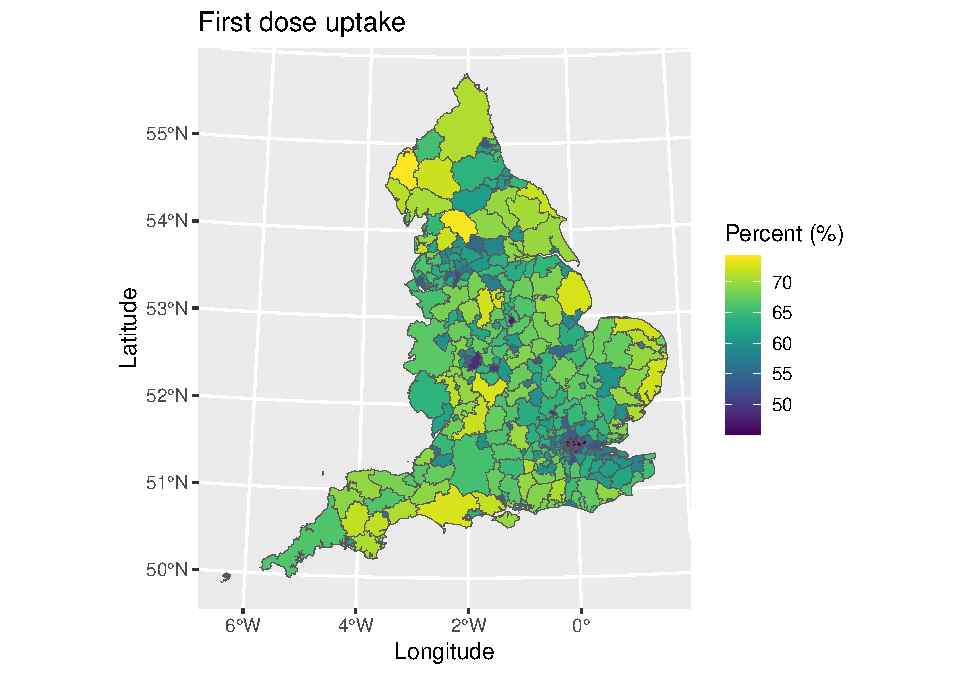
\includegraphics{Spatial-Data_files/figure-latex/unnamed-chunk-41-1.pdf}

What are the main spatial patterns that you can observe? There is lower uptake in urban areas, especially London, although many of these areas are small on the map due taking up smaller land mass. Else, there is probably not any other distinct spatial pattern.

\hypertarget{non-spatial-regression}{%
\section{Non-spatial regression}\label{non-spatial-regression}}

If we wanted to understand why uptake was higher or lower in certain areas, we might use a regression model. If we focus on the standard OLS regression model, we utilise the following equation:

\[
y = X\beta + \epsilon
\]

Here, we predict \(y\) as a function of a series of predictor \(X\) variables that we adjust their effects based on \(\beta\) values and some measure of the error \(\epsilon\). We can use an OLS regression model to help us explain patterns in uptake, based on our explanatory variables.

\begin{Shaded}
\begin{Highlighting}[]
\NormalTok{model1 }\OtherTok{\textless{}{-}} \FunctionTok{lm}\NormalTok{(percent\_first\_dose }\SpecialCharTok{\textasciitilde{}}\NormalTok{ median\_age }\SpecialCharTok{+}\NormalTok{ Other\_White }\SpecialCharTok{+}\NormalTok{ Mixed }\SpecialCharTok{+}\NormalTok{ Black }\SpecialCharTok{+}\NormalTok{ Asian }\SpecialCharTok{+}\NormalTok{ Other }\SpecialCharTok{+}\NormalTok{ mean\_imd\_score }\SpecialCharTok{+}\NormalTok{ pop\_density, }\AttributeTok{data =}\NormalTok{ lad\_eng) }\CommentTok{\# Fit a linear regression model for the following equation (outcome \textasciitilde{} explanatory)}
\FunctionTok{summary}\NormalTok{(model1) }\CommentTok{\# Print model results summary}
\end{Highlighting}
\end{Shaded}

\begin{verbatim}
## 
## Call:
## lm(formula = percent_first_dose ~ median_age + Other_White + 
##     Mixed + Black + Asian + Other + mean_imd_score + pop_density, 
##     data = lad_eng)
## 
## Residuals:
##      Min       1Q   Median       3Q      Max 
## -11.0686  -1.3129  -0.1212   1.2518   7.0054 
## 
## Coefficients:
##                  Estimate Std. Error t value Pr(>|t|)    
## (Intercept)     3.203e+01  2.113e+00  15.155  < 2e-16 ***
## median_age      8.150e-01  4.255e-02  19.155  < 2e-16 ***
## Other_White    -7.320e-02  4.555e-02  -1.607   0.1091    
## Mixed           4.014e-01  1.589e-01   2.526   0.0120 *  
## Black          -2.516e-01  5.138e-02  -4.896 1.58e-06 ***
## Asian           1.910e-02  2.139e-02   0.893   0.3724    
## Other          -1.406e-01  1.100e-01  -1.278   0.2021    
## mean_imd_score -9.943e-02  1.925e-02  -5.166 4.31e-07 ***
## pop_density    -2.440e-04  9.955e-05  -2.451   0.0148 *  
## ---
## Signif. codes:  0 '***' 0.001 '**' 0.01 '*' 0.05 '.' 0.1 ' ' 1
## 
## Residual standard error: 2.287 on 308 degrees of freedom
## Multiple R-squared:  0.8612, Adjusted R-squared:  0.8576 
## F-statistic: 238.9 on 8 and 308 DF,  p-value: < 2.2e-16
\end{verbatim}

Urgh, what ugly output. I mean it is functional, but not pretty. Good thing we can make the output nicer using various packages in R. I really like \texttt{gtsummary} which can clean regression tables up.

\begin{Shaded}
\begin{Highlighting}[]
\FunctionTok{library}\NormalTok{(gtsummary) }\CommentTok{\# Load package}
\NormalTok{tbl\_model1 }\OtherTok{\textless{}{-}} \FunctionTok{tbl\_regression}\NormalTok{(model1, }\AttributeTok{label =} \FunctionTok{list}\NormalTok{(median\_age }\SpecialCharTok{\textasciitilde{}} \StringTok{"Median age"}\NormalTok{, Other\_White }\SpecialCharTok{\textasciitilde{}} \StringTok{"Other White (\%)"}\NormalTok{, Mixed }\SpecialCharTok{\textasciitilde{}} \StringTok{"Mixed (\%)"}\NormalTok{, Black }\SpecialCharTok{\textasciitilde{}} \StringTok{"Black (\%)"}\NormalTok{, Asian }\SpecialCharTok{\textasciitilde{}} \StringTok{"Asian (\%)"}\NormalTok{, Other }\SpecialCharTok{\textasciitilde{}} \StringTok{"Other Ethnicity (\%)"}\NormalTok{, mean\_imd\_score }\SpecialCharTok{\textasciitilde{}} \StringTok{"Deprivation score"}\NormalTok{, pop\_density }\SpecialCharTok{\textasciitilde{}} \StringTok{"Population density"}\NormalTok{)) }\CommentTok{\# Make tidy table}
\NormalTok{tbl\_model1 }\CommentTok{\# Print}
\end{Highlighting}
\end{Shaded}

\begin{tabular}{l|l|l|l}
\hline
**Characteristic** & **Beta** & **95\% CI** & **p-value**\\
\hline
Median age & 0.81 & 0.73, 0.90 & <0.001\\
\hline
Other White (\%) & -0.07 & -0.16, 0.02 & 0.11\\
\hline
Mixed (\%) & 0.40 & 0.09, 0.71 & 0.012\\
\hline
Black (\%) & -0.25 & -0.35, -0.15 & <0.001\\
\hline
Asian (\%) & 0.02 & -0.02, 0.06 & 0.4\\
\hline
Other Ethnicity (\%) & -0.14 & -0.36, 0.08 & 0.2\\
\hline
Deprivation score & -0.10 & -0.14, -0.06 & <0.001\\
\hline
Population density & 0.00 & 0.00, 0.00 & 0.015\\
\hline
\end{tabular}

What does the model say?

\begin{itemize}
\tightlist
\item
  Median age was positively associated with the percentage of the population who were vaccinated, with areas that had older populations on average being associated with higher uptake.
\item
  There are mixed associations found for the ethnicity variables - a negative association between the percentage of an area's population that were Black or Black British and uptake (i.e., uptake was lower in areas with a higher share of the population that were Black), a positive association between Mixed ethnicity and uptake, and large uncertainty in estimates for `Asian', `Other White' or `Other Ethnicity' communities.
\item
  Deprivation score was negatively associated with uptake, where as areas became more deprived uptake was lower.
\item
  The effect for population density looks misleading in the cleaned table due to rounding issues, but if we scroll back up to the messier table we can see that as population density increases (i.e., larger more populated urban areas) uptake falls
\end{itemize}

A few questions for you to think about: Was this the correct statistical model? Were the correct explanatory variables used and what happens if you try others? Does the same associations persist if we look at second dose uptake?

One of the classical assumptions of an OLS regression model is the independence of errors (and to some extent observations as well). Since we have spatial data and areas closer together may be similar than those further apart (i.e., the characteristics and populations of Liverpool and Wirral are more similar than say, Liverpool and Guildford), this assumption may not hold. We can assess if this may be an issue through plotting the residuals (i.e., our error term \(\epsilon\)) from the regression model and exploring if any spatial patterns exist.

\begin{Shaded}
\begin{Highlighting}[]
\CommentTok{\# Join on }
\NormalTok{lad\_eng }\OtherTok{\textless{}{-}} \FunctionTok{cbind}\NormalTok{(lad\_eng, model1}\SpecialCharTok{$}\NormalTok{residuals)}

\CommentTok{\# Plot}
\NormalTok{map2 }\OtherTok{\textless{}{-}} \FunctionTok{ggplot}\NormalTok{() }\SpecialCharTok{+} \CommentTok{\# Call ggplot command}
  \FunctionTok{geom\_sf}\NormalTok{(}\AttributeTok{data =}\NormalTok{ lad\_eng, }\FunctionTok{aes}\NormalTok{(}\AttributeTok{fill =}\NormalTok{ model1.residuals), }\AttributeTok{lwd =} \DecValTok{0}\NormalTok{) }\SpecialCharTok{+} \CommentTok{\# Define what to plot}
  \FunctionTok{scale\_fill\_viridis}\NormalTok{() }\SpecialCharTok{+} \CommentTok{\# Make colourblind friendly}
  \FunctionTok{xlab}\NormalTok{(}\StringTok{"Longitude"}\NormalTok{) }\SpecialCharTok{+} \CommentTok{\# Add x{-}axis label}
  \FunctionTok{ylab}\NormalTok{(}\StringTok{"Latitude"}\NormalTok{) }\SpecialCharTok{+} \CommentTok{\# Add y{-}axis label}
  \FunctionTok{labs}\NormalTok{(}\AttributeTok{title =} \StringTok{"First dose uptake model"}\NormalTok{, }\CommentTok{\# Edit plot title}
       \AttributeTok{fill =} \StringTok{"Residuals"}\NormalTok{) }\CommentTok{\# Edit legend title}
\NormalTok{map2 }\CommentTok{\# Print plot}
\end{Highlighting}
\end{Shaded}

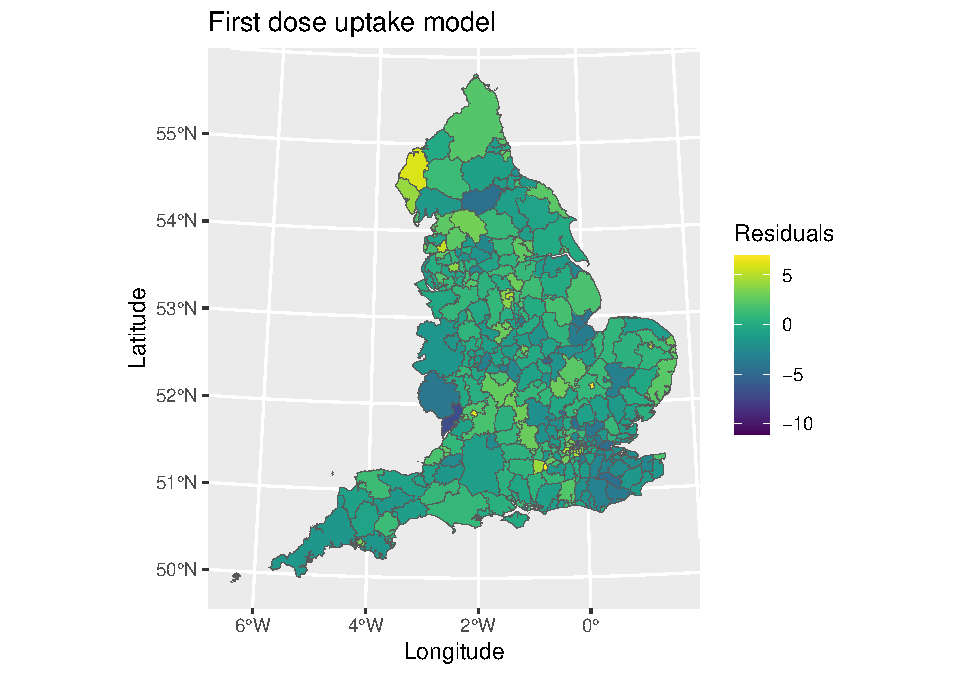
\includegraphics{Spatial-Data_files/figure-latex/unnamed-chunk-44-1.pdf}

If there were no issues here, we might expect to find a random pattern. However, we can see this isn't always the case. A positive residual would suggest that the observed value of an area is greater than what the model would predict based on the coefficients and it's local values for each explanatory variable. There are some clustering of values in the North West, London and other urban areas. Similarly, a negative value suggests lower observed uptake than we might expect/predict from the model. We can see evidence of this in the West and South East of England.

Our analysis may therefore benefit from having a spatial regression model.

\hypertarget{selecting-the-right-spatial-model}{%
\section{Selecting the right spatial model}\label{selecting-the-right-spatial-model}}

The first thing we might want to check is the extent that there is spatial clustering of our data. We will start here by checking this for our outcome variable and the regression model residuals. We will follow the same methods that we introduced in the \protect\hyperlink{cluster}{previous session}.

We will need to identify the spatial structure of our dataset. We will follow the same previous method of assigning neighbouring areas based on Queen's contiguity. One issue here is that we have two Local Authorities that are islands (Isles of Scilly and Isle of Wight) which do not have any neighbours. To solve this, we could either assign the two islands manually to their nearest `neighbour' (e.g., Isles of Scilly to Cornwall) or remove them from our analysis. For the basis of teaching you the methods here \sout{and because I am too lazy to code it up as it is a faff}, we will just remove them from the data. We ought to re-run our regression model since we are dropping two observations, but we will not to save time here (we will correct this later so stay tuned).

Let's check the spatial clustering in our outcome variable through calculating the Moran's I.

\begin{Shaded}
\begin{Highlighting}[]
\FunctionTok{library}\NormalTok{(spdep) }\CommentTok{\# Load package}
\NormalTok{lad\_eng }\OtherTok{\textless{}{-}}\NormalTok{ lad\_eng[lad\_eng}\SpecialCharTok{$}\NormalTok{lad19cd }\SpecialCharTok{!=} \StringTok{"E06000053"} \SpecialCharTok{\&}\NormalTok{ lad\_eng}\SpecialCharTok{$}\NormalTok{lad19cd }\SpecialCharTok{!=} \StringTok{"E06000046"}\NormalTok{,] }\CommentTok{\# Drop Isles of Scilly or Isle of Wight}
\NormalTok{nb }\OtherTok{\textless{}{-}} \FunctionTok{poly2nb}\NormalTok{(lad\_eng, }\AttributeTok{queen =} \ConstantTok{TRUE}\NormalTok{) }\CommentTok{\# Calculate queen contiguity for areas (slow)}
\NormalTok{lw }\OtherTok{\textless{}{-}} \FunctionTok{nb2listw}\NormalTok{(nb, }\AttributeTok{style =} \StringTok{"W"}\NormalTok{, }\AttributeTok{zero.policy =} \ConstantTok{TRUE}\NormalTok{) }\CommentTok{\# Assign weights based on list of neighbours}
\NormalTok{m1 }\OtherTok{\textless{}{-}} \FunctionTok{moran.test}\NormalTok{(lad\_eng}\SpecialCharTok{$}\NormalTok{percent\_first\_dose, lw) }\CommentTok{\# Calculate Moran\textquotesingle{}s I}
\NormalTok{m1 }\CommentTok{\# Print result}
\end{Highlighting}
\end{Shaded}

\begin{verbatim}
## 
##  Moran I test under randomisation
## 
## data:  lad_eng$percent_first_dose  
## weights: lw    
## 
## Moran I statistic standard deviate = 11.055, p-value < 2.2e-16
## alternative hypothesis: greater
## sample estimates:
## Moran I statistic       Expectation          Variance 
##       0.407962351      -0.003184713       0.001383250
\end{verbatim}

A Moran's I value of 0.4079624 would indicate existence of moderate spatial clustering of first COVID-19 vaccination dose uptake.

Next, we will repeat the analysis for the regression model residuals. Remember this is more important in checking the model assumptions.

\begin{Shaded}
\begin{Highlighting}[]
\NormalTok{m2 }\OtherTok{\textless{}{-}} \FunctionTok{moran.test}\NormalTok{(lad\_eng}\SpecialCharTok{$}\NormalTok{model1.residuals, lw) }\CommentTok{\# Calculate Moran\textquotesingle{}s I}
\NormalTok{m2 }\CommentTok{\# Print result}
\end{Highlighting}
\end{Shaded}

\begin{verbatim}
## 
##  Moran I test under randomisation
## 
## data:  lad_eng$model1.residuals  
## weights: lw    
## 
## Moran I statistic standard deviate = 7.4067, p-value = 6.476e-14
## alternative hypothesis: greater
## sample estimates:
## Moran I statistic       Expectation          Variance 
##       0.271550385      -0.003184713       0.001375889
\end{verbatim}

Here, a value of 0.2715504 suggests weak clustering. While low, the result is statistically significant suggesting it is important variation that we need to take in account in how we approach our regression analysis.

Do you think that was a bit of a faff to code up? Well, you can do the whole thing in a single line of code thanks to \texttt{spdep}'s \texttt{lm.morantest} command. Indeed, it can allow us to update our regression model with the dropped observations quickly too. \sout{OK I should I have said this earlier to not waste your time, but sorry not sorry as it is useful to show the manual process I hope.}

\begin{Shaded}
\begin{Highlighting}[]
\NormalTok{model1 }\OtherTok{\textless{}{-}} \FunctionTok{lm}\NormalTok{(percent\_first\_dose }\SpecialCharTok{\textasciitilde{}}\NormalTok{ median\_age }\SpecialCharTok{+}\NormalTok{ Other\_White }\SpecialCharTok{+}\NormalTok{ Mixed }\SpecialCharTok{+}\NormalTok{ Black }\SpecialCharTok{+}\NormalTok{ Asian }\SpecialCharTok{+}\NormalTok{ Other }\SpecialCharTok{+}\NormalTok{ mean\_imd\_score }\SpecialCharTok{+}\NormalTok{ pop\_density, }\AttributeTok{data =}\NormalTok{ lad\_eng) }\CommentTok{\# Re{-}run regression model}
\NormalTok{m3 }\OtherTok{\textless{}{-}} \FunctionTok{lm.morantest}\NormalTok{(model1, lw) }\CommentTok{\# Run Moran\textquotesingle{}s I analysis of residuals}
\NormalTok{m3 }\CommentTok{\# Print results}
\end{Highlighting}
\end{Shaded}

\begin{verbatim}
## 
##  Global Moran I for regression residuals
## 
## data:  
## model: lm(formula = percent_first_dose ~ median_age + Other_White + Mixed + Black + Asian
## + Other + mean_imd_score + pop_density, data = lad_eng)
## weights: lw
## 
## Moran I statistic standard deviate = 7.6783, p-value = 8.061e-15
## alternative hypothesis: greater
## sample estimates:
## Observed Moran I      Expectation         Variance 
##      0.271337873     -0.010969132      0.001351802
\end{verbatim}

Again we get a similar result.

So we have a problem. How might we address it? It might be that we have left out some unmeasured explanatory covariates that would account for the spatial variation. This might not always be possible. A different approach would be to account for the spatial structure of our underlying dataset. We could do this by adding in a categorical variable representing each area as a fixed effect in the regression model. You can try this by re-running the previous code and adding into the formula \texttt{lad19cd} - what are the issues this brings? We could also extend this model to be a multi-level regression model where the area identifier is specified as a random effect (check out R package \texttt{lme4} for more here). Neither of these models explicitly accounts for the spatial nature of the data (i.e., the regression model does not know the spatial structure of the data).

The other thing we could do is use a spatial regression model that explicitly accounts for the locations of each data point. Here we tell the regression model that the spatial structure of data points matters for their interpretation (i.e., data points closer to each other are more similar than those further apart). There are \emph{a lot} of different types of spatial regression models. How might we select the correct model?

Selection of models may be based on which specification we think best describes our data. This is hard to decide! The other approach is that we can utilise model fit statistics to assess which spatial models may improve upon the OLS regression model we previously fit. We can do this using \texttt{spdep}'s \texttt{lm.LMtests} function. Here we test for different features of \textbf{spatial dependence} in our data/model. For review here, please consult the lecture slides for this practical \href{}{located here}. Tl;dr spatial dependence is where the spatial configuration (i.e., structure of locations) affects our outcome.

We will focus in this practical on spatial lag and spatial error models. The following code tests for whether a spatially lagged dependent variable or spatial error dependence can improve our model fit. We can test for more things using this code, but for now we stick with these four tests.

\begin{Shaded}
\begin{Highlighting}[]
\NormalTok{spat\_dep\_test }\OtherTok{\textless{}{-}} \FunctionTok{lm.LMtests}\NormalTok{(model1, lw, }\AttributeTok{test=}\FunctionTok{c}\NormalTok{(}\StringTok{"LMerr"}\NormalTok{, }\StringTok{"LMlag"}\NormalTok{, }\StringTok{"RLMerr"}\NormalTok{, }\StringTok{"RLMlag"}\NormalTok{)) }\CommentTok{\# Test for spatial dependence}
\NormalTok{spat\_dep\_test}
\end{Highlighting}
\end{Shaded}

\begin{verbatim}
## 
##  Lagrange multiplier diagnostics for spatial dependence
## 
## data:  
## model: lm(formula = percent_first_dose ~ median_age + Other_White + Mixed + Black + Asian
## + Other + mean_imd_score + pop_density, data = lad_eng)
## weights: lw
## 
## LMerr = 52.31, df = 1, p-value = 4.738e-13
## 
## 
##  Lagrange multiplier diagnostics for spatial dependence
## 
## data:  
## model: lm(formula = percent_first_dose ~ median_age + Other_White + Mixed + Black + Asian
## + Other + mean_imd_score + pop_density, data = lad_eng)
## weights: lw
## 
## LMlag = 37.432, df = 1, p-value = 9.466e-10
## 
## 
##  Lagrange multiplier diagnostics for spatial dependence
## 
## data:  
## model: lm(formula = percent_first_dose ~ median_age + Other_White + Mixed + Black + Asian
## + Other + mean_imd_score + pop_density, data = lad_eng)
## weights: lw
## 
## RLMerr = 24.317, df = 1, p-value = 8.171e-07
## 
## 
##  Lagrange multiplier diagnostics for spatial dependence
## 
## data:  
## model: lm(formula = percent_first_dose ~ median_age + Other_White + Mixed + Black + Asian
## + Other + mean_imd_score + pop_density, data = lad_eng)
## weights: lw
## 
## RLMlag = 9.4386, df = 1, p-value = 0.002125
\end{verbatim}

If we consider all of the tests, we can see that for each test of spatial dependence that they are each statistically significant. This would suggest that each spatial model can benefit our analysis and model fit. If none were significant, then we would use the OLS regression results.

\hypertarget{spatial-lag-model}{%
\section{Spatial lag model}\label{spatial-lag-model}}

The first types of spatial models we will consider are those which incorporate a \textbf{spatial lag}. These models use variables that are spatially lagged, which means that they calculate measures for each area that characterise (e.g., mean value) their surrounding neighbours. Spatial lags might correspond to the outcome variable or explanatory variables. A spatial lag suggests that the surrounding areas have an influence on the outcome of an area.

\hypertarget{slx-spatially-lagged-model}{%
\subsection{SLX spatially lagged model}\label{slx-spatially-lagged-model}}

The first spatial regression model we will consider is the \textbf{SLX spatial lag model}. SLX here means Spatially Lagged X-variables. We define the model as:

\[
y = X \beta + WX \theta + \epsilon
\]

The equation is a simple extension of the OLS regression equation. Our outcome variable \(y\) is a function of our explanatory variables \(X\) and their \(\beta\) coefficients, a spatial lag coefficient \(\theta\) of the \(X\) variables based on a spatial weight \(W\) and the error term \(\epsilon\). The \(\beta\) value represents the \emph{direct effect} of an explanatory variable and the \(\theta\) value represents the \emph{indirect effect}. An indirect effect is synonymous with a \emph{spillover effect} whereby changes in \(x\) in an area have on it's surrounding neighbours based on how \(W\) is defined. The spatial lags are exogenous in definition.

To fit the model, we use the R package \texttt{spatialreg} which allows us to fit cross-sectional spatial regression models. We re-run the previous analysis of first dose uptake using this spatial model and tidy the output (please note that \texttt{gtsummary} does not handle spatial models well).

\begin{Shaded}
\begin{Highlighting}[]
\FunctionTok{library}\NormalTok{(spatialreg) }\CommentTok{\# Load package}
\NormalTok{model2 }\OtherTok{\textless{}{-}} \FunctionTok{lmSLX}\NormalTok{(percent\_first\_dose }\SpecialCharTok{\textasciitilde{}}\NormalTok{ median\_age }\SpecialCharTok{+}\NormalTok{ Other\_White }\SpecialCharTok{+}\NormalTok{ Mixed }\SpecialCharTok{+}\NormalTok{ Black }\SpecialCharTok{+}\NormalTok{ Asian }\SpecialCharTok{+}\NormalTok{ Other }\SpecialCharTok{+}\NormalTok{ mean\_imd\_score }\SpecialCharTok{+}\NormalTok{ pop\_density, }\AttributeTok{data =}\NormalTok{ lad\_eng, lw) }\CommentTok{\# Spatial lag model}
\NormalTok{tbl\_model2 }\OtherTok{\textless{}{-}} \FunctionTok{tbl\_regression}\NormalTok{(model2, }\AttributeTok{label =} \FunctionTok{list}\NormalTok{(median\_age }\SpecialCharTok{\textasciitilde{}} \StringTok{"Median age"}\NormalTok{, Other\_White }\SpecialCharTok{\textasciitilde{}} \StringTok{"Other White (\%)"}\NormalTok{, Mixed }\SpecialCharTok{\textasciitilde{}} \StringTok{"Mixed (\%)"}\NormalTok{, Black }\SpecialCharTok{\textasciitilde{}} \StringTok{"Black (\%)"}\NormalTok{, Asian }\SpecialCharTok{\textasciitilde{}} \StringTok{"Asian (\%)"}\NormalTok{, Other }\SpecialCharTok{\textasciitilde{}} \StringTok{"Other Ethnicity (\%)"}\NormalTok{, mean\_imd\_score }\SpecialCharTok{\textasciitilde{}} \StringTok{"Deprivation score"}\NormalTok{, pop\_density }\SpecialCharTok{\textasciitilde{}} \StringTok{"Population density"}\NormalTok{, lag.median\_age }\SpecialCharTok{\textasciitilde{}} \StringTok{"Lag: Median age"}\NormalTok{, lag.Other\_White }\SpecialCharTok{\textasciitilde{}} \StringTok{"Lag: Other White (\%)"}\NormalTok{, lag.Mixed }\SpecialCharTok{\textasciitilde{}} \StringTok{"Lag: Mixed (\%)"}\NormalTok{, lag.Black }\SpecialCharTok{\textasciitilde{}} \StringTok{"Lag: Black (\%)"}\NormalTok{, lag.Asian }\SpecialCharTok{\textasciitilde{}} \StringTok{"Lag: Asian (\%)"}\NormalTok{, lag.Other }\SpecialCharTok{\textasciitilde{}} \StringTok{"Lag: Other Ethnicity (\%)"}\NormalTok{, lag.mean\_imd\_score }\SpecialCharTok{\textasciitilde{}} \StringTok{"Lag: Deprivation score"}\NormalTok{, lag.pop\_density }\SpecialCharTok{\textasciitilde{}} \StringTok{"Lag: Population density"}\NormalTok{)) }\CommentTok{\# Tidy model output}
\NormalTok{tbl\_model2 }\CommentTok{\# Print}
\end{Highlighting}
\end{Shaded}

\begin{tabular}{l|l|l|l}
\hline
**Characteristic** & **Beta** & **95\% CI** & **p-value**\\
\hline
Median age & 0.90 & 0.81, 1.0 & <0.001\\
\hline
Other White (\%) & -0.08 & -0.19, 0.03 & 0.2\\
\hline
Mixed (\%) & 0.31 & -0.01, 0.62 & 0.055\\
\hline
Black (\%) & -0.17 & -0.29, -0.06 & 0.003\\
\hline
Asian (\%) & 0.02 & -0.03, 0.07 & 0.4\\
\hline
Other Ethnicity (\%) & -0.01 & -0.24, 0.23 & >0.9\\
\hline
Deprivation score & -0.10 & -0.15, -0.04 & <0.001\\
\hline
Population density & 0.00 & 0.00, 0.00 & 0.4\\
\hline
Lag: Median age & -0.07 & -0.22, 0.09 & 0.4\\
\hline
Lag: Other White (\%) & 0.04 & -0.16, 0.23 & 0.7\\
\hline
Lag: Mixed (\%) & 0.48 & -0.14, 1.1 & 0.13\\
\hline
Lag: Black (\%) & -0.22 & -0.45, 0.00 & 0.052\\
\hline
Lag: Asian (\%) & 0.04 & -0.06, 0.13 & 0.4\\
\hline
Lag: Other Ethnicity (\%) & -0.19 & -0.68, 0.29 & 0.4\\
\hline
Lag: Deprivation score & -0.01 & -0.09, 0.06 & 0.7\\
\hline
Lag: Population density & 0.00 & 0.00, 0.00 & 0.046\\
\hline
\end{tabular}

To interpret the model can be difficult. The \(\beta\) coefficients are not exactly the same. Rather, to understand the marginal effect of our covariates, we need to estimate their total impacts (i.e., direct effect + indirect effect). To do this, we use the following piece of code.

\begin{Shaded}
\begin{Highlighting}[]
\NormalTok{model2\_imp }\OtherTok{\textless{}{-}} \FunctionTok{impacts}\NormalTok{(model2, }\AttributeTok{listw =}\NormalTok{ lw) }\CommentTok{\# Estimate direct, indirect and total effects of variables}
\NormalTok{model2\_imp }\CommentTok{\# Print}
\end{Highlighting}
\end{Shaded}

\begin{verbatim}
## Impact measures (SLX, estimable):
##                       Direct      Indirect         Total
## median_age      0.9009090557 -0.0696177362  0.8312913196
## Other_White    -0.0790245349  0.0358434195 -0.0431811154
## Mixed           0.3057806432  0.4837927431  0.7895733864
## Black          -0.1732816347 -0.2225162881 -0.3957979227
## Asian           0.0188294285  0.0374534457  0.0562828742
## Other          -0.0058036010 -0.1928748969 -0.1986784979
## mean_imd_score -0.0971854562 -0.0125373425 -0.1097227986
## pop_density     0.0001022996 -0.0004974955 -0.0003951959
\end{verbatim}

You will see here these are exactly the same as \(\beta\) coefficients for this model, however this will not always be the case. What is useful here is that we can see the direct impact in an area, the indirect effects surrounding each and the total effect of each factor considering both together. The spatial lags here are mostly non-statistically significant, other than for population density. It suggests that they bring little to the model.

Standard errors and p-values for these statistics can be estimated through the following modified version of the code.

\begin{Shaded}
\begin{Highlighting}[]
\NormalTok{model2\_imp\_se }\OtherTok{\textless{}{-}} \FunctionTok{summary}\NormalTok{(}\FunctionTok{impacts}\NormalTok{(model2, lw), }\AttributeTok{zstats =} \ConstantTok{TRUE}\NormalTok{) }\CommentTok{\# Estimate}
\NormalTok{model2\_imp\_se }\CommentTok{\# Print}
\end{Highlighting}
\end{Shaded}

\begin{verbatim}
## Impact measures (SLX, estimable, n-k):
##                       Direct      Indirect         Total
## median_age      0.9009090557 -0.0696177362  0.8312913196
## Other_White    -0.0790245349  0.0358434195 -0.0431811154
## Mixed           0.3057806432  0.4837927431  0.7895733864
## Black          -0.1732816347 -0.2225162881 -0.3957979227
## Asian           0.0188294285  0.0374534457  0.0562828742
## Other          -0.0058036010 -0.1928748969 -0.1986784979
## mean_imd_score -0.0971854562 -0.0125373425 -0.1097227986
## pop_density     0.0001022996 -0.0004974955 -0.0003951959
## ========================================================
## Standard errors:
##                      Direct     Indirect        Total
## median_age     0.0479267084 0.0788605699 0.0759959852
## Other_White    0.0554022011 0.1005400225 0.0903636892
## Mixed          0.1589370191 0.3165363389 0.3306975306
## Black          0.0588396940 0.1139981394 0.1050719658
## Asian          0.0236130613 0.0476175809 0.0435460352
## Other          0.1174828586 0.2470964358 0.2521944956
## mean_imd_score 0.0268712927 0.0388509279 0.0305507387
## pop_density    0.0001209284 0.0002482232 0.0002218059
## ========================================================
## Z-values:
##                     Direct   Indirect      Total
## median_age     18.79764092 -0.8827952 10.9386215
## Other_White    -1.42637898  0.3565090 -0.4778591
## Mixed           1.92391077  1.5283956  2.3875999
## Black          -2.94497851 -1.9519291 -3.7669222
## Asian           0.79741581  0.7865466  1.2924914
## Other          -0.04939956 -0.7805653 -0.7877987
## mean_imd_score -3.61670192 -0.3227038 -3.5914941
## pop_density     0.84595204 -2.0042263 -1.7817198
## 
## p-values:
##                Direct     Indirect Total     
## median_age     < 2.22e-16 0.377347 < 2.22e-16
## Other_White    0.15375898 0.721459 0.63275046
## Mixed          0.05436577 0.126414 0.01695879
## Black          0.00322977 0.050947 0.00016527
## Asian          0.42520958 0.431547 0.19618704
## Other          0.96060088 0.435058 0.43081446
## mean_imd_score 0.00029838 0.746920 0.00032879
## pop_density    0.39757950 0.045046 0.07479493
\end{verbatim}

We can also compare the results from the spatial model to our original OLS regression model

\begin{Shaded}
\begin{Highlighting}[]
\FunctionTok{tbl\_merge}\NormalTok{(}\FunctionTok{list}\NormalTok{(tbl\_model1, tbl\_model2)) }\CommentTok{\# Combine both model outputs together}
\end{Highlighting}
\end{Shaded}

\begin{tabular}{l|l|l|l|l|l|l}
\hline
**Characteristic** & **Beta** & **95\% CI** & **p-value** & **Beta** & **95\% CI** & **p-value**\\
\hline
Median age & 0.81 & 0.73, 0.90 & <0.001 & 0.90 & 0.81, 1.0 & <0.001\\
\hline
Other White (\%) & -0.07 & -0.16, 0.02 & 0.11 & -0.08 & -0.19, 0.03 & 0.2\\
\hline
Mixed (\%) & 0.40 & 0.09, 0.71 & 0.012 & 0.31 & -0.01, 0.62 & 0.055\\
\hline
Black (\%) & -0.25 & -0.35, -0.15 & <0.001 & -0.17 & -0.29, -0.06 & 0.003\\
\hline
Asian (\%) & 0.02 & -0.02, 0.06 & 0.4 & 0.02 & -0.03, 0.07 & 0.4\\
\hline
Other Ethnicity (\%) & -0.14 & -0.36, 0.08 & 0.2 & -0.01 & -0.24, 0.23 & >0.9\\
\hline
Deprivation score & -0.10 & -0.14, -0.06 & <0.001 & -0.10 & -0.15, -0.04 & <0.001\\
\hline
Population density & 0.00 & 0.00, 0.00 & 0.015 & 0.00 & 0.00, 0.00 & 0.4\\
\hline
Lag: Median age &  &  &  & -0.07 & -0.22, 0.09 & 0.4\\
\hline
Lag: Other White (\%) &  &  &  & 0.04 & -0.16, 0.23 & 0.7\\
\hline
Lag: Mixed (\%) &  &  &  & 0.48 & -0.14, 1.1 & 0.13\\
\hline
Lag: Black (\%) &  &  &  & -0.22 & -0.45, 0.00 & 0.052\\
\hline
Lag: Asian (\%) &  &  &  & 0.04 & -0.06, 0.13 & 0.4\\
\hline
Lag: Other Ethnicity (\%) &  &  &  & -0.19 & -0.68, 0.29 & 0.4\\
\hline
Lag: Deprivation score &  &  &  & -0.01 & -0.09, 0.06 & 0.7\\
\hline
Lag: Population density &  &  &  & 0.00 & 0.00, 0.00 & 0.046\\
\hline
\end{tabular}

Not a lot has changed if we compare the direct effects of coefficients (many remain within their 95\% confidence intervals), probably because the spatial lagged effects were not strong or identifiable. Population density has become non-statistically significant mind you, as has percentage of people who with mixed ethnicity.

We can also compare model fit to see if the spatial model improves on the original OLS regression model. For example, we can check this by quickly looking at the AIC model fit.

\begin{Shaded}
\begin{Highlighting}[]
\FunctionTok{AIC}\NormalTok{(model1) }\CommentTok{\# OLS regression model}
\end{Highlighting}
\end{Shaded}

\begin{verbatim}
## [1] 1424.31
\end{verbatim}

\begin{Shaded}
\begin{Highlighting}[]
\FunctionTok{AIC}\NormalTok{(model2) }\CommentTok{\# SLX spatial lag model}
\end{Highlighting}
\end{Shaded}

\begin{verbatim}
## [1] 1406.79
\end{verbatim}

The spatial lag model does improve model fit overall.

\hypertarget{sar-spatial-lag}{%
\subsection{SAR Spatial Lag}\label{sar-spatial-lag}}

The other spatial lag model that we can specify is the following:

\[
y = \rho Wy + X\beta + \epsilon
\]

SAR stands for Spatial AutoRegressive model. Here, we have the standard OLS regression equation \(X\beta + \epsilon\), however we also have included a spatial lag component \(\rho W\) of our outcome variable \(y\). \(W\) is once again our spatial weights matrix, with \(\rho\) representing the correlation of the spatial lag of \(y\) to \(y\).

Since the model contains \(y\) at both sides of the equation, it violates the exogeneity assumption of the OLS regression model. We therefore need a different approach to estimate the equation.

Please note: \texttt{gtsummary} does not handle spatial models well, so we will have to \sout{fudge it} persist a bit here. If you can fix it, send your answers on a postcard/carrier pigeon please. Remember, you can always get the raw output of a model by using \texttt{summary(model3)}.

\begin{Shaded}
\begin{Highlighting}[]
\NormalTok{model3 }\OtherTok{\textless{}{-}} \FunctionTok{lagsarlm}\NormalTok{(percent\_first\_dose }\SpecialCharTok{\textasciitilde{}}\NormalTok{ median\_age }\SpecialCharTok{+}\NormalTok{ Other\_White }\SpecialCharTok{+}\NormalTok{ Mixed }\SpecialCharTok{+}\NormalTok{ Black }\SpecialCharTok{+}\NormalTok{ Asian }\SpecialCharTok{+}\NormalTok{ Other }\SpecialCharTok{+}\NormalTok{ mean\_imd\_score }\SpecialCharTok{+}\NormalTok{ pop\_density, }\AttributeTok{data =}\NormalTok{ lad\_eng, lw) }\CommentTok{\# Model}
\NormalTok{tbl\_model3 }\OtherTok{\textless{}{-}} \FunctionTok{tbl\_regression}\NormalTok{(model3) }\CommentTok{\# Tidy model output}
\NormalTok{tbl\_model3 }\CommentTok{\# Print}
\end{Highlighting}
\end{Shaded}

\begin{tabular}{l|l|l|l}
\hline
**Characteristic** & **Beta** & **95\% CI** & **p-value**\\
\hline
rho & 0.23 & 0.16, 0.29 & <0.001\\
\hline
(Intercept) & 16 & 10, 22 & <0.001\\
\hline
median\_age & 0.84 & 0.76, 0.92 & <0.001\\
\hline
Other\_White & -0.09 & -0.17, -0.01 & 0.029\\
\hline
Mixed & 0.39 & 0.10, 0.68 & 0.008\\
\hline
Black & -0.17 & -0.26, -0.07 & <0.001\\
\hline
Asian & 0.04 & 0.00, 0.08 & 0.044\\
\hline
Other & -0.04 & -0.24, 0.16 & 0.7\\
\hline
mean\_imd\_score & -0.11 & -0.15, -0.08 & <0.001\\
\hline
pop\_density & 0.00 & 0.00, 0.00 & 0.15\\
\hline
\end{tabular}

Let's compare it to our standard OLS regression model. We will go back to the untidy version of the output to match the above

\begin{Shaded}
\begin{Highlighting}[]
\NormalTok{tbl\_model1 }\OtherTok{\textless{}{-}} \FunctionTok{tbl\_regression}\NormalTok{(model1, }\AttributeTok{intercept =} \ConstantTok{TRUE}\NormalTok{) }\CommentTok{\# Redo Table 1 to match above format}
\FunctionTok{tbl\_merge}\NormalTok{(}\AttributeTok{tbls =} \FunctionTok{list}\NormalTok{(tbl\_model1, tbl\_model3), }\CommentTok{\# Join output together}
          \AttributeTok{tab\_spanner =} \FunctionTok{c}\NormalTok{(}\StringTok{"**OLS**"}\NormalTok{, }\StringTok{"**Spatial Lag**"}\NormalTok{)) }\CommentTok{\# Rename columns (in bold)}
\end{Highlighting}
\end{Shaded}

\begin{verbatim}
## Table printed with `knitr::kable()`, not {gt}. Learn why at
## http://www.danieldsjoberg.com/gtsummary/articles/rmarkdown.html
## To suppress this message, include `message = FALSE` in code chunk header.
\end{verbatim}

\begin{tabular}{l|l|l|l|l|l|l}
\hline
**Characteristic** & **Beta** & **95\% CI** & **p-value** & **Beta** & **95\% CI** & **p-value**\\
\hline
(Intercept) & 32 & 28, 36 & <0.001 & 16 & 10, 22 & <0.001\\
\hline
median\_age & 0.81 & 0.73, 0.90 & <0.001 & 0.84 & 0.76, 0.92 & <0.001\\
\hline
Other\_White & -0.07 & -0.16, 0.02 & 0.13 & -0.09 & -0.17, -0.01 & 0.029\\
\hline
Mixed & 0.42 & 0.10, 0.73 & 0.009 & 0.39 & 0.10, 0.68 & 0.008\\
\hline
Black & -0.25 & -0.36, -0.15 & <0.001 & -0.17 & -0.26, -0.07 & <0.001\\
\hline
Asian & 0.02 & -0.02, 0.06 & 0.4 & 0.04 & 0.00, 0.08 & 0.044\\
\hline
Other & -0.14 & -0.36, 0.07 & 0.2 & -0.04 & -0.24, 0.16 & 0.7\\
\hline
mean\_imd\_score & -0.10 & -0.14, -0.06 & <0.001 & -0.11 & -0.15, -0.08 & <0.001\\
\hline
pop\_density & 0.00 & 0.00, 0.00 & 0.013 & 0.00 & 0.00, 0.00 & 0.15\\
\hline
rho &  &  &  & 0.23 & 0.16, 0.29 & <0.001\\
\hline
\end{tabular}

Not a lot has changed between the models, suggesting that the spatial patterns captured very little of the patterns observed in our covariates. The most interesting difference is for our population density variable \texttt{pop\_density}, which has gone from statistically significant in our OLS regression model to insignificant in our spatial lag model. The percentage of people with their ethnicity as other White (\texttt{Other\_White}) has now become statistically significant as well, with a negative association to the percentage vaccinated. Otherwise, the coefficients have remained similar and within the 95\% Confidence Intervals of the OLS estimates.

The summary output for the spatial lag model gives us only the direct impacts for our coefficients, however we may be interested in the direct, indirect and total effects each covariate is having on our outcome variable.

\begin{Shaded}
\begin{Highlighting}[]
\FunctionTok{impacts}\NormalTok{(model3, }\AttributeTok{listw =}\NormalTok{ lw) }\CommentTok{\# Estimate direct and indirect effects}
\end{Highlighting}
\end{Shaded}

\begin{verbatim}
## Impact measures (lag, exact):
##                       Direct      Indirect         Total
## median_age      0.8509693217  2.364693e-01  1.0874386629
## Other_White    -0.0930566879 -2.585881e-02 -0.1189154975
## Mixed           0.3929949698  1.092064e-01  0.5022013292
## Black          -0.1678335124 -4.663797e-02 -0.2144714806
## Asian           0.0406973608  1.130908e-02  0.0520064384
## Other          -0.0389923533 -1.083529e-02 -0.0498276394
## mean_imd_score -0.1152847834 -3.203560e-02 -0.1473203881
## pop_density    -0.0001353991 -3.762503e-05 -0.0001730242
\end{verbatim}

The table would suggest that the indirect effects of each covariate on the surrounding areas means that focusing on the direct association alone underestimates the total impact of each variable.

To get the standard errors and p-values for our direct, indirect and total effects, we use the following code. Unlike the SLX model, we cannot estimate these directly and therefore must use simulations (MCMC) approaches to estimate them. This only requires a slight modification to the code, in our case we will add in 500 simulations (the more the merrier, but impacts on processing time).

\begin{Shaded}
\begin{Highlighting}[]
\FunctionTok{summary}\NormalTok{(}\FunctionTok{impacts}\NormalTok{(model3, }\AttributeTok{listw =}\NormalTok{ lw, }\AttributeTok{R =} \DecValTok{500}\NormalTok{), }\AttributeTok{zstats =} \ConstantTok{TRUE}\NormalTok{) }\CommentTok{\# Slow, but gives quantiles etc}
\end{Highlighting}
\end{Shaded}

\begin{verbatim}
## Impact measures (lag, exact):
##                       Direct      Indirect         Total
## median_age      0.8509693217  2.364693e-01  1.0874386629
## Other_White    -0.0930566879 -2.585881e-02 -0.1189154975
## Mixed           0.3929949698  1.092064e-01  0.5022013292
## Black          -0.1678335124 -4.663797e-02 -0.2144714806
## Asian           0.0406973608  1.130908e-02  0.0520064384
## Other          -0.0389923533 -1.083529e-02 -0.0498276394
## mean_imd_score -0.1152847834 -3.203560e-02 -0.1473203881
## pop_density    -0.0001353991 -3.762503e-05 -0.0001730242
## ========================================================
## Simulation results (asymptotic variance matrix):
## Direct:
## 
## Iterations = 1:500
## Thinning interval = 1 
## Number of chains = 1 
## Sample size per chain = 500 
## 
## 1. Empirical mean and standard deviation for each variable,
##    plus standard error of the mean:
## 
##                     Mean        SD  Naive SE Time-series SE
## median_age      0.848966 4.059e-02 1.815e-03      1.815e-03
## Other_White    -0.092037 4.159e-02 1.860e-03      1.860e-03
## Mixed           0.395293 1.481e-01 6.623e-03      6.623e-03
## Black          -0.167725 4.847e-02 2.168e-03      2.168e-03
## Asian           0.038972 2.090e-02 9.346e-04      9.346e-04
## Other          -0.043215 1.013e-01 4.532e-03      4.532e-03
## mean_imd_score -0.115206 1.846e-02 8.255e-04      9.266e-04
## pop_density    -0.000135 9.561e-05 4.276e-06      4.276e-06
## 
## 2. Quantiles for each variable:
## 
##                      2.5%        25%        50%        75%      97.5%
## median_age      0.7664745  0.8226682  0.8487204  8.762e-01  9.209e-01
## Other_White    -0.1723514 -0.1186415 -0.0928376 -6.540e-02 -6.619e-04
## Mixed           0.1130657  0.2949465  0.3928388  4.880e-01  6.840e-01
## Black          -0.2615833 -0.2014520 -0.1661371 -1.344e-01 -7.364e-02
## Asian          -0.0003528  0.0249858  0.0383172  5.491e-02  8.006e-02
## Other          -0.2355007 -0.1118957 -0.0490080  1.836e-02  1.668e-01
## mean_imd_score -0.1512615 -0.1264853 -0.1146608 -1.037e-01 -7.597e-02
## pop_density    -0.0003118 -0.0001989 -0.0001358 -7.152e-05  5.842e-05
## 
## ========================================================
## Indirect:
## 
## Iterations = 1:500
## Thinning interval = 1 
## Number of chains = 1 
## Sample size per chain = 500 
## 
## 1. Empirical mean and standard deviation for each variable,
##    plus standard error of the mean:
## 
##                      Mean        SD  Naive SE Time-series SE
## median_age      2.383e-01 4.742e-02 2.121e-03      2.121e-03
## Other_White    -2.606e-02 1.315e-02 5.880e-04      5.880e-04
## Mixed           1.111e-01 4.625e-02 2.068e-03      2.068e-03
## Black          -4.661e-02 1.522e-02 6.807e-04      6.807e-04
## Asian           1.106e-02 6.630e-03 2.965e-04      2.774e-04
## Other          -1.115e-02 2.899e-02 1.297e-03      1.297e-03
## mean_imd_score -3.254e-02 9.019e-03 4.033e-04      4.033e-04
## pop_density    -3.695e-05 2.707e-05 1.211e-06      1.211e-06
## 
## 2. Quantiles for each variable:
## 
##                      2.5%        25%        50%        75%      97.5%
## median_age      1.525e-01  2.068e-01  2.343e-01  0.2697871  3.374e-01
## Other_White    -5.482e-02 -3.439e-02 -2.544e-02 -0.0170469 -1.855e-04
## Mixed           2.785e-02  7.778e-02  1.078e-01  0.1414005  2.079e-01
## Black          -8.027e-02 -5.543e-02 -4.494e-02 -0.0360156 -1.893e-02
## Asian          -6.441e-05  6.655e-03  1.069e-02  0.0148835  2.414e-02
## Other          -6.490e-02 -2.899e-02 -1.327e-02  0.0049522  5.086e-02
## mean_imd_score -5.047e-02 -3.824e-02 -3.143e-02 -0.0264686 -1.663e-02
## pop_density    -9.208e-05 -5.505e-05 -3.763e-05 -0.0000199  1.639e-05
## 
## ========================================================
## Total:
## 
## Iterations = 1:500
## Thinning interval = 1 
## Number of chains = 1 
## Sample size per chain = 500 
## 
## 1. Empirical mean and standard deviation for each variable,
##    plus standard error of the mean:
## 
##                      Mean        SD  Naive SE Time-series SE
## median_age      1.0872632 0.0704481 3.151e-03      3.151e-03
## Other_White    -0.1180927 0.0539240 2.412e-03      2.412e-03
## Mixed           0.5063599 0.1902076 8.506e-03      8.506e-03
## Black          -0.2143314 0.0613835 2.745e-03      2.745e-03
## Asian           0.0500308 0.0271325 1.213e-03      1.213e-03
## Other          -0.0543686 0.1297901 5.804e-03      5.804e-03
## mean_imd_score -0.1477435 0.0257326 1.151e-03      1.275e-03
## pop_density    -0.0001719 0.0001217 5.441e-06      5.441e-06
## 
## 2. Quantiles for each variable:
## 
##                      2.5%        25%        50%        75%      97.5%
## median_age      0.9537914  1.0365970  1.0866387  1.134e+00  1.2294100
## Other_White    -0.2257873 -0.1524865 -0.1193417 -8.563e-02 -0.0008475
## Mixed           0.1377256  0.3735414  0.5072748  6.273e-01  0.8849579
## Black          -0.3353566 -0.2554803 -0.2109999 -1.713e-01 -0.0956411
## Asian          -0.0004385  0.0318691  0.0490388  6.857e-02  0.1044283
## Other          -0.2959382 -0.1409078 -0.0620159  2.308e-02  0.2132935
## mean_imd_score -0.1974803 -0.1641138 -0.1467182 -1.321e-01 -0.0957729
## pop_density    -0.0003889 -0.0002513 -0.0001739 -9.378e-05  0.0000763
## 
## ========================================================
## Simulated standard errors
##                      Direct     Indirect        Total
## median_age     4.058575e-02 4.742005e-02 0.0704481412
## Other_White    4.158862e-02 1.314826e-02 0.0539239806
## Mixed          1.480980e-01 4.624582e-02 0.1902076123
## Black          4.847404e-02 1.522061e-02 0.0613834517
## Asian          2.089903e-02 6.630289e-03 0.0271324845
## Other          1.013431e-01 2.899309e-02 0.1297900785
## mean_imd_score 1.845863e-02 9.018901e-03 0.0257325714
## pop_density    9.561299e-05 2.707167e-05 0.0001216605
## 
## Simulated z-values:
##                    Direct   Indirect      Total
## median_age     20.9178385  5.0252382 15.4335253
## Other_White    -2.2130248 -1.9817142 -2.1899856
## Mixed           2.6691337  2.4016552  2.6621432
## Black          -3.4601040 -3.0620438 -3.4916804
## Asian           1.8647712  1.6679352  1.8439449
## Other          -0.4264235 -0.3846967 -0.4188967
## mean_imd_score -6.2412962 -3.6077324 -5.7414995
## pop_density    -1.4114253 -1.3647544 -1.4129222
## 
## Simulated p-values:
##                Direct     Indirect   Total     
## median_age     < 2.22e-16 5.0281e-07 < 2.22e-16
## Other_White    0.02689594 0.04751124 0.02852528
## Mixed          0.00760472 0.01632109 0.00776448
## Black          0.00053997 0.00219831 0.00047999
## Asian          0.06221348 0.09532858 0.06519118
## Other          0.66979928 0.70046211 0.67529166
## mean_imd_score 4.3396e-10 0.00030888 9.3842e-09
## pop_density    0.15811924 0.17233027 0.15767861
\end{verbatim}

It gives a lot of output, but it is useful to pick apart how useful our estimates are.

\hypertarget{spatial-error-models}{%
\section{Spatial error models}\label{spatial-error-models}}

We next explore how to implement spatial error models. The underlying models are modified OLS regression models meaning the models are more straightforward ways of accounting for spatial processes in our analysis, as well as being fairly easy to interpret. In this section, we will deal with models that incorporate the spatial structure of the dataset within the error terms. Remember that this was the key OLS assumption that might have been violated (i.e., independence of errors).

\hypertarget{spatial-error-model-sem}{%
\subsection{Spatial Error Model (SEM)}\label{spatial-error-model-sem}}

The main equation that we are trying to estimate in our spatial error model is:

\[
y = X\beta + u
\]

Here, we are trying to explain our outcome variable \(y\) based upon our the \(\beta\) coefficients of covariate variables \(X\) plus our error term \(u\). The equation itself looks fairly similar to the OLS equation, until we introduce the spatial autocorrelation element to our model. We partition \(u\) into the following:

\[
u = \lambda Wu + \epsilon
\]

We define \(u\) as a coefficient \(\lambda\) controlling the spatial weight \(W\) placed on the the error terms \(u\), plus the general error term \(\epsilon\) for our model.

We cannot use the OLS regression model to estimate the equation, since the assumption of independence of error terms is violated. We therefore require new approaches to do this. Again, \texttt{gtsummary} doesn't like these types of models but I have included here as it helps clean the output up.

\begin{Shaded}
\begin{Highlighting}[]
\NormalTok{model4 }\OtherTok{\textless{}{-}} \FunctionTok{errorsarlm}\NormalTok{(percent\_first\_dose }\SpecialCharTok{\textasciitilde{}}\NormalTok{ median\_age }\SpecialCharTok{+}\NormalTok{ Other\_White }\SpecialCharTok{+}\NormalTok{ Mixed }\SpecialCharTok{+}\NormalTok{ Black }\SpecialCharTok{+}\NormalTok{ Asian }\SpecialCharTok{+}\NormalTok{ Other }\SpecialCharTok{+}\NormalTok{ mean\_imd\_score }\SpecialCharTok{+}\NormalTok{ pop\_density, }\AttributeTok{data =}\NormalTok{ lad\_eng, lw) }\CommentTok{\# Model}
\NormalTok{tbl\_model4 }\OtherTok{\textless{}{-}} \FunctionTok{tbl\_regression}\NormalTok{(model4) }\CommentTok{\# Tidy model output}
\end{Highlighting}
\end{Shaded}

\begin{verbatim}
## x Unable to identify the list of variables.
## 
## This is usually due to an error calling `stats::model.frame(x)`or `stats::model.matrix(x)`.
## It could be the case if that type of model does not implement these methods.
## Rarely, this error may occur if the model object was created within
## a functional programming framework (e.g. using `lappy()`, `purrr::map()`, etc.).
\end{verbatim}

\begin{Shaded}
\begin{Highlighting}[]
\NormalTok{tbl\_model4 }\CommentTok{\# Print}
\end{Highlighting}
\end{Shaded}

\begin{verbatim}
## Table printed with `knitr::kable()`, not {gt}. Learn why at
## http://www.danieldsjoberg.com/gtsummary/articles/rmarkdown.html
## To suppress this message, include `message = FALSE` in code chunk header.
\end{verbatim}

\begin{tabular}{l|l|l|l}
\hline
**Characteristic** & **Beta** & **95\% CI** & **p-value**\\
\hline
(Intercept) & 29 & 25, 33 & <0.001\\
\hline
median\_age & 0.87 & 0.79, 0.95 & <0.001\\
\hline
Other\_White & -0.11 & -0.19, -0.02 & 0.020\\
\hline
Mixed & 0.24 & -0.03, 0.51 & 0.078\\
\hline
Black & -0.19 & -0.28, -0.09 & <0.001\\
\hline
Asian & 0.01 & -0.03, 0.05 & 0.5\\
\hline
Other & 0.00 & -0.20, 0.19 & >0.9\\
\hline
mean\_imd\_score & -0.08 & -0.12, -0.04 & <0.001\\
\hline
pop\_density & 0.00 & 0.00, 0.00 & 0.6\\
\hline
lambda & 0.62 & 0.51, 0.72 & <0.001\\
\hline
\end{tabular}

These models do not have direct and indirect effects since the spatial component only affects the error term.

We may also want to check whether a spatial error model was relevant here through running a \textbf{Hausman Test} which compares if the model improves upon the OLS model.

\begin{Shaded}
\begin{Highlighting}[]
\NormalTok{HausmanTest }\OtherTok{\textless{}{-}} \FunctionTok{Hausman.test}\NormalTok{(model4) }\CommentTok{\# Run test}
\NormalTok{HausmanTest }\CommentTok{\# Print}
\end{Highlighting}
\end{Shaded}

\begin{verbatim}
## 
##  Spatial Hausman test (asymptotic)
## 
## data:  NULL
## Hausman test = 21.562, df = 9, p-value = 0.01038
\end{verbatim}

The test suggests that the spatial error improves the model (i.e., we want it to be statistically significant).

We can compare the model output to the OLS and spatial lag models too.

\begin{Shaded}
\begin{Highlighting}[]
\FunctionTok{tbl\_merge}\NormalTok{(}\AttributeTok{tbls =} \FunctionTok{list}\NormalTok{(tbl\_model1, tbl\_model3, tbl\_model4), }\CommentTok{\# Join three model outputs together}
          \AttributeTok{tab\_spanner =} \FunctionTok{c}\NormalTok{(}\StringTok{"**OLS**"}\NormalTok{, }\StringTok{"**Spatial Lag**"}\NormalTok{, }\StringTok{"**Spatial Error**"}\NormalTok{)) }\CommentTok{\# Rename columns (in bold)}
\end{Highlighting}
\end{Shaded}

\begin{tabular}{l|l|l|l|l|l|l|l|l|l}
\hline
**Characteristic** & **Beta** & **95\% CI** & **p-value** & **Beta** & **95\% CI** & **p-value** & **Beta** & **95\% CI** & **p-value**\\
\hline
(Intercept) & 32 & 28, 36 & <0.001 & 16 & 10, 22 & <0.001 & 29 & 25, 33 & <0.001\\
\hline
median\_age & 0.81 & 0.73, 0.90 & <0.001 & 0.84 & 0.76, 0.92 & <0.001 & 0.87 & 0.79, 0.95 & <0.001\\
\hline
Other\_White & -0.07 & -0.16, 0.02 & 0.13 & -0.09 & -0.17, -0.01 & 0.029 & -0.11 & -0.19, -0.02 & 0.020\\
\hline
Mixed & 0.42 & 0.10, 0.73 & 0.009 & 0.39 & 0.10, 0.68 & 0.008 & 0.24 & -0.03, 0.51 & 0.078\\
\hline
Black & -0.25 & -0.36, -0.15 & <0.001 & -0.17 & -0.26, -0.07 & <0.001 & -0.19 & -0.28, -0.09 & <0.001\\
\hline
Asian & 0.02 & -0.02, 0.06 & 0.4 & 0.04 & 0.00, 0.08 & 0.044 & 0.01 & -0.03, 0.05 & 0.5\\
\hline
Other & -0.14 & -0.36, 0.07 & 0.2 & -0.04 & -0.24, 0.16 & 0.7 & 0.00 & -0.20, 0.19 & >0.9\\
\hline
mean\_imd\_score & -0.10 & -0.14, -0.06 & <0.001 & -0.11 & -0.15, -0.08 & <0.001 & -0.08 & -0.12, -0.04 & <0.001\\
\hline
pop\_density & 0.00 & 0.00, 0.00 & 0.013 & 0.00 & 0.00, 0.00 & 0.15 & 0.00 & 0.00, 0.00 & 0.6\\
\hline
rho &  &  &  & 0.23 & 0.16, 0.29 & <0.001 &  &  & \\
\hline
lambda &  &  &  &  &  &  & 0.62 & 0.51, 0.72 & <0.001\\
\hline
\end{tabular}

The spatial error model looks relatively similar to the spatial lag model, although there are some differences with \texttt{Mixed} and \texttt{Asian} variables now being statistically insignificant.

\hypertarget{spatial-durbin-error}{%
\subsection{Spatial Durbin Error}\label{spatial-durbin-error}}

We can extend the spatial error model through adding in spatial lags for our x-variables, accounting for the spatial effects of independent variables. This requires only a minor modification of the spatial error model equation:

\[
y = X\beta + WX\theta + u
\]
The key difference to the spatial error model is the introduction of \(WX\theta\) which applies the spatial weight \(W\) to the independent variables \(X\) and our spatial autocorrelation coefficient \(\theta\).

\(u\) again is defined as:

\[
u = \lambda Wu + \epsilon
\]

We can fit this model using a slight change to the spatial error code. Please note that \texttt{gtsummary} does not like this type of model output either, so it is a little messy again.

\begin{Shaded}
\begin{Highlighting}[]
\NormalTok{model5 }\OtherTok{\textless{}{-}} \FunctionTok{errorsarlm}\NormalTok{(percent\_first\_dose }\SpecialCharTok{\textasciitilde{}}\NormalTok{ median\_age }\SpecialCharTok{+}\NormalTok{ Other\_White }\SpecialCharTok{+}\NormalTok{ Mixed }\SpecialCharTok{+}\NormalTok{ Black }\SpecialCharTok{+}\NormalTok{ Asian }\SpecialCharTok{+}\NormalTok{ Other }\SpecialCharTok{+}\NormalTok{ mean\_imd\_score }\SpecialCharTok{+}\NormalTok{ pop\_density, }\AttributeTok{data =}\NormalTok{ lad\_eng, lw, }\AttributeTok{etype =} \StringTok{"emixed"}\NormalTok{) }\CommentTok{\# Fit model}
\NormalTok{tbl\_model5 }\OtherTok{\textless{}{-}} \FunctionTok{tbl\_regression}\NormalTok{(model5) }\CommentTok{\# Tidy model output}
\NormalTok{tbl\_model5 }\CommentTok{\# Print}
\end{Highlighting}
\end{Shaded}

\begin{tabular}{l|l|l|l}
\hline
**Characteristic** & **Beta** & **95\% CI** & **p-value**\\
\hline
(Intercept) & 31 & 22, 41 & <0.001\\
\hline
median\_age & 0.91 & 0.83, 1.0 & <0.001\\
\hline
Other\_White & -0.10 & -0.19, -0.01 & 0.034\\
\hline
Mixed & 0.28 & 0.00, 0.57 & 0.049\\
\hline
Black & -0.20 & -0.30, -0.10 & <0.001\\
\hline
Asian & 0.02 & -0.02, 0.06 & 0.4\\
\hline
Other & 0.00 & -0.20, 0.21 & >0.9\\
\hline
mean\_imd\_score & -0.07 & -0.11, -0.03 & 0.001\\
\hline
pop\_density & 0.00 & 0.00, 0.00 & 0.6\\
\hline
lag.median\_age & -0.08 & -0.25, 0.08 & 0.3\\
\hline
lag.Other\_White & 0.08 & -0.14, 0.29 & 0.5\\
\hline
lag.Mixed & 0.62 & -0.04, 1.3 & 0.064\\
\hline
lag.Black & -0.11 & -0.35, 0.14 & 0.4\\
\hline
lag.Asian & 0.02 & -0.08, 0.12 & 0.7\\
\hline
lag.Other & -0.38 & -0.93, 0.16 & 0.2\\
\hline
lag.mean\_imd\_score & -0.06 & -0.14, 0.02 & 0.14\\
\hline
lag.pop\_density & 0.00 & 0.00, 0.00 & 0.15\\
\hline
lambda & 0.55 & 0.43, 0.66 & <0.001\\
\hline
\end{tabular}

The inclusion of spatial lags does not seem to bring much advantage here. Since we have introduced spatial lags into our model, we can also calculate the direct, indirect and total effects of covariates too. I have included the code for calculating standard errors, however we don't need to run it again \sout{because I am lazy}.

\begin{Shaded}
\begin{Highlighting}[]
\FunctionTok{impacts}\NormalTok{(model5, }\AttributeTok{listw =}\NormalTok{ lw) }\CommentTok{\# Calculate indirect, direct and total effects}
\end{Highlighting}
\end{Shaded}

\begin{verbatim}
## Impact measures (SDEM, estimable):
##                       Direct      Indirect         Total
## median_age      9.115621e-01 -0.0841690665  0.8273930013
## Other_White    -9.924527e-02  0.0753496736 -0.0238955924
## Mixed           2.834532e-01  0.6242855916  0.9077388144
## Black          -2.041149e-01 -0.1070505848 -0.3111654388
## Asian           1.583933e-02  0.0209621790  0.0368015073
## Other           3.784383e-03 -0.3849049537 -0.3811205710
## mean_imd_score -7.049241e-02 -0.0594952812 -0.1299876895
## pop_density     5.783698e-05 -0.0003724632 -0.0003146262
\end{verbatim}

\begin{Shaded}
\begin{Highlighting}[]
\CommentTok{\# summary(impacts(model3, listw = lw, R = 500), zstats = TRUE) \# Slow, but gives quantiles, standard errors and p{-}values}
\end{Highlighting}
\end{Shaded}

There are more extensions of these models \sout{than you can shake a stick at} we could explore here - for example, SARAR or SARMA - and most of them are essentially different combinations of spatial lags and spatial error models. We can save them for a rainy day.

\hypertarget{summary-2}{%
\section{Summary}\label{summary-2}}

In this practical session, we have explored how to extend the standard OLS regression model to incorporate spatial processes. We will continue this theme in the next, and final, session where we examine Geographically Weighted Regression.

\hypertarget{gwr}{%
\chapter{Geographically Weighted Regression}\label{gwr}}

In our last session (boo), we extend the spatial regression approach to explore the concept of spatially varying coefficients. The lecture slides for this practical can be found \href{}{here}. A PDF version of the practical can be found \href{}{here}.

\hypertarget{loading-data}{%
\section{Loading data}\label{loading-data}}

We will use the same data introduced in the \href{\%7B\#spatreg\%7D}{previous session}. We will this time look at second dose uptake to mix it up. Let's quickly load in the data and tidy it.

\begin{Shaded}
\begin{Highlighting}[]
\CommentTok{\# Load package}
\FunctionTok{library}\NormalTok{(sf)}

\CommentTok{\# Load and clean spatial data}
\NormalTok{lad\_uk }\OtherTok{\textless{}{-}} \FunctionTok{read\_sf}\NormalTok{(}\StringTok{"./Shapefiles/UK\_LAD/Local\_Authority\_Districts\_(December\_2019)\_Boundaries\_UK\_BFC.shp"}\NormalTok{) }\CommentTok{\# Load shapefile for Local Authority Districts (LADs) for UK (sorry but could not find only England version so need to convert to match data)}
\NormalTok{lad\_uk}\SpecialCharTok{$}\NormalTok{country }\OtherTok{\textless{}{-}} \FunctionTok{substr}\NormalTok{(lad\_uk}\SpecialCharTok{$}\NormalTok{lad19cd, }\DecValTok{0}\NormalTok{, }\DecValTok{1}\NormalTok{) }\CommentTok{\# Record first letter of LAD code (denotes country)}
\NormalTok{lad\_eng }\OtherTok{\textless{}{-}}\NormalTok{ lad\_uk[lad\_uk}\SpecialCharTok{$}\NormalTok{country }\SpecialCharTok{==} \StringTok{"E"}\NormalTok{,] }\CommentTok{\# Subset only English LADs}

\CommentTok{\# Tidy and join on explanatory variables}
\NormalTok{lad\_data }\OtherTok{\textless{}{-}} \FunctionTok{read.csv}\NormalTok{(}\StringTok{"./Data/LAD\_vaccine\_data.csv"}\NormalTok{) }\CommentTok{\# Load vaccine uptake and demographic data for England}
\NormalTok{lad\_eng }\OtherTok{\textless{}{-}} \FunctionTok{merge}\NormalTok{(lad\_eng, lad\_data, }\AttributeTok{by.x =} \StringTok{"lad19cd"}\NormalTok{, }\AttributeTok{by.y =} \StringTok{"ltla\_code"}\NormalTok{, }\AttributeTok{all.x =} \ConstantTok{TRUE}\NormalTok{) }\CommentTok{\# Join on both datasets}
\NormalTok{lad\_eng}\SpecialCharTok{$}\NormalTok{pop\_density }\OtherTok{\textless{}{-}}\NormalTok{ lad\_eng}\SpecialCharTok{$}\NormalTok{population }\SpecialCharTok{/}\NormalTok{ (lad\_eng}\SpecialCharTok{$}\NormalTok{st\_areasha }\SpecialCharTok{/} \DecValTok{1000000}\NormalTok{) }\CommentTok{\# Calculate population density (st\_areashape is measured in metres\^{}2 so need to convert to km\^{}2 by dividing by 1,000,000)}
\NormalTok{lad\_eng}\SpecialCharTok{$}\NormalTok{percent\_first\_dose }\OtherTok{\textless{}{-}}\NormalTok{ (lad\_eng}\SpecialCharTok{$}\NormalTok{total\_first\_dose }\SpecialCharTok{/}\NormalTok{ lad\_eng}\SpecialCharTok{$}\NormalTok{population) }\SpecialCharTok{*} \DecValTok{100} \CommentTok{\# Calculate percent of population who have had their first dose}
\NormalTok{lad\_eng}\SpecialCharTok{$}\NormalTok{percent\_second\_dose }\OtherTok{\textless{}{-}}\NormalTok{ (lad\_eng}\SpecialCharTok{$}\NormalTok{total\_second\_dose }\SpecialCharTok{/}\NormalTok{ lad\_eng}\SpecialCharTok{$}\NormalTok{population) }\SpecialCharTok{*} \DecValTok{100} \CommentTok{\# Calculate percent of population who have had their first dose}

\CommentTok{\# Remove objects to save space}
\FunctionTok{rm}\NormalTok{(lad\_uk, lad\_data) }
\end{Highlighting}
\end{Shaded}

Let's have a look at the spatial pattern of the variable.

\begin{Shaded}
\begin{Highlighting}[]
\CommentTok{\# Load packages}
\FunctionTok{library}\NormalTok{(ggplot2) }
\FunctionTok{library}\NormalTok{(viridis)}

\CommentTok{\# Plot}
\NormalTok{map1 }\OtherTok{\textless{}{-}} \FunctionTok{ggplot}\NormalTok{() }\SpecialCharTok{+} \CommentTok{\# Call ggplot command}
  \FunctionTok{geom\_sf}\NormalTok{(}\AttributeTok{data =}\NormalTok{ lad\_eng, }\FunctionTok{aes}\NormalTok{(}\AttributeTok{fill =}\NormalTok{ percent\_second\_dose), }\AttributeTok{lwd =} \DecValTok{0}\NormalTok{) }\SpecialCharTok{+} \CommentTok{\# Define what to plot}
  \FunctionTok{scale\_fill\_viridis}\NormalTok{() }\SpecialCharTok{+} \CommentTok{\# Make colourblind friendly}
  \FunctionTok{xlab}\NormalTok{(}\StringTok{"Longitude"}\NormalTok{) }\SpecialCharTok{+} \CommentTok{\# Add x{-}axis label}
  \FunctionTok{ylab}\NormalTok{(}\StringTok{"Latitude"}\NormalTok{) }\SpecialCharTok{+} \CommentTok{\# Add y{-}axis label}
  \FunctionTok{labs}\NormalTok{(}\AttributeTok{title =} \StringTok{"Second dose uptake"}\NormalTok{, }\CommentTok{\# Edit plot title}
       \AttributeTok{fill =} \StringTok{"Percent (\%)"}\NormalTok{) }\CommentTok{\# Edit legend title}
\NormalTok{map1 }\CommentTok{\# Print plot}
\end{Highlighting}
\end{Shaded}

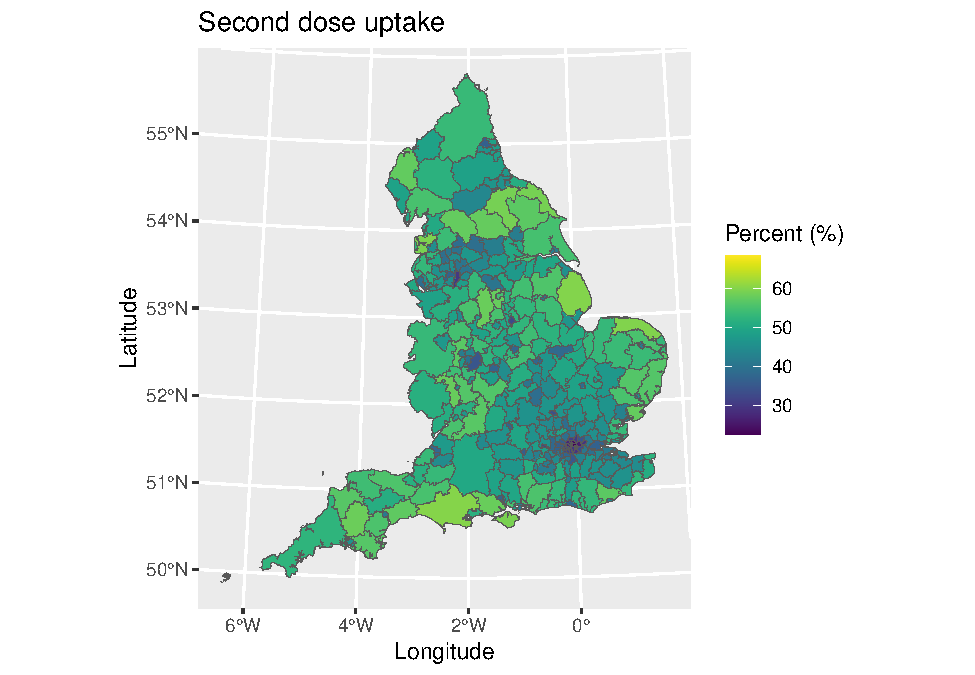
\includegraphics{Spatial-Data_files/figure-latex/unnamed-chunk-64-1.pdf}

We can see lower uptake in urban areas and higher uptake in rural regions. This is likely reflecting differences in the age-structure of areas.

Let's use a standard linear regression model to examine the factors that are associated with the percentage of individuals who are fully vaccinated (i.e., received their second vaccine dose). This will be useful to compare to the \textbf{Geographically Weighted Regression (GWR)} model later.

\begin{Shaded}
\begin{Highlighting}[]
\NormalTok{model1 }\OtherTok{\textless{}{-}} \FunctionTok{lm}\NormalTok{(percent\_second\_dose }\SpecialCharTok{\textasciitilde{}}\NormalTok{ median\_age }\SpecialCharTok{+}\NormalTok{ Other\_White }\SpecialCharTok{+}\NormalTok{ Mixed }\SpecialCharTok{+}\NormalTok{ Black }\SpecialCharTok{+}\NormalTok{ Asian }\SpecialCharTok{+}\NormalTok{ Other }\SpecialCharTok{+}\NormalTok{ mean\_imd\_score }\SpecialCharTok{+}\NormalTok{ pop\_density, }\AttributeTok{data =}\NormalTok{ lad\_eng) }\CommentTok{\# OLS model}
\FunctionTok{summary}\NormalTok{(model1) }\CommentTok{\# Print model results}
\end{Highlighting}
\end{Shaded}

\begin{verbatim}
## 
## Call:
## lm(formula = percent_second_dose ~ median_age + Other_White + 
##     Mixed + Black + Asian + Other + mean_imd_score + pop_density, 
##     data = lad_eng)
## 
## Residuals:
##      Min       1Q   Median       3Q      Max 
## -17.9897  -1.5236  -0.1079   1.4989  14.1068 
## 
## Coefficients:
##                  Estimate Std. Error t value Pr(>|t|)    
## (Intercept)     4.7972830  2.4171174   1.985 0.048063 *  
## median_age      1.0410090  0.0486634  21.392  < 2e-16 ***
## Other_White    -0.1070692  0.0520983  -2.055 0.040709 *  
## Mixed           0.1228759  0.1817387   0.676 0.499476    
## Black          -0.1811159  0.0587695  -3.082 0.002243 ** 
## Asian          -0.0259803  0.0244621  -1.062 0.289039    
## Other          -0.1225451  0.1258458  -0.974 0.330934    
## mean_imd_score  0.0204583  0.0220153   0.929 0.353474    
## pop_density    -0.0004277  0.0001139  -3.756 0.000206 ***
## ---
## Signif. codes:  0 '***' 0.001 '**' 0.01 '*' 0.05 '.' 0.1 ' ' 1
## 
## Residual standard error: 2.616 on 308 degrees of freedom
## Multiple R-squared:  0.8804, Adjusted R-squared:  0.8773 
## F-statistic: 283.5 on 8 and 308 DF,  p-value: < 2.2e-16
\end{verbatim}

The model results suggest the following associations:

\begin{itemize}
\tightlist
\item
  Median age of a Local Authority is positively associated with the percentage of the population who have had their second vaccine dose, so that older populations had more fully vaccinated individuals
\item
  Greater percentages of areas with Black or Other White ethnic groups had lower uptake, with a negative association detected.
\item
  Population density was negatively associated to vaccination uptake, with uptake decreasing with increasing population density.
\end{itemize}

\hypertarget{selecting-bandwidths}{%
\section{Selecting bandwidths}\label{selecting-bandwidths}}

GWR is a technique that allows us to examine how associations between variables may vary across space. It works through selecting a `search window' (here defined as surrounding areas) over each data point (Local Authority District in our example), estimating a regression equation (for the data point and data points in the search window, with closer neighbouring data points given larger weightings), and then repeating the process for all data points. This means the process estimates \emph{n} regression equations each time (you can probably see here how it can become computationally intensive). The result is a series of regression coefficients for each variable and each area, allowing us to explore how coefficients vary across space.

To be able to estimate a model, we need to define the `search window'. This consists of two components: (i) a spatial kernel, and (ii) bandwidth. The \textbf{spatial kernel} refers to the weighting mechanism that gives greater importance/weighting to data points located closer to each data point (and vice versa), and the extent that the weighting changes with distance. The kernel can be fixed (i.e., the same bandwidth, such as a fixed distance, is used for each regression) or adaptive (i.e., varying bandwidths are used, such as nearest number of neighbours). \textbf{Bandwidith} is the extent of the kernel (i.e., how big an area it covers).

We can optimise the bandwidth value using a cross-validation. Here we estimate a regression model for a particular location with a set bandwidth value. We then compare the predicted outcome value for the model to the observed/actual value, which gives us the residual error. We can then vary the bandwidth value and see how the residual changes, with the aim of minimising it.

\begin{Shaded}
\begin{Highlighting}[]
\FunctionTok{library}\NormalTok{(spgwr) }\CommentTok{\# Load package}
\end{Highlighting}
\end{Shaded}

\begin{verbatim}
## NOTE: This package does not constitute approval of GWR
## as a method of spatial analysis; see example(gwr)
\end{verbatim}

\begin{Shaded}
\begin{Highlighting}[]
\NormalTok{fixed\_bandwidth }\OtherTok{\textless{}{-}} \FunctionTok{gwr.sel}\NormalTok{(percent\_second\_dose }\SpecialCharTok{\textasciitilde{}}\NormalTok{ median\_age }\SpecialCharTok{+}\NormalTok{ Other\_White }\SpecialCharTok{+}\NormalTok{ Mixed }\SpecialCharTok{+}\NormalTok{ Black }\SpecialCharTok{+}\NormalTok{ Asian }\SpecialCharTok{+}\NormalTok{ Other }\SpecialCharTok{+}\NormalTok{ mean\_imd\_score }\SpecialCharTok{+}\NormalTok{ pop\_density, }\AttributeTok{data =}\NormalTok{ lad\_eng, }\AttributeTok{coords =} \FunctionTok{cbind}\NormalTok{(lad\_eng}\SpecialCharTok{$}\NormalTok{long, lad\_eng}\SpecialCharTok{$}\NormalTok{lat), }\AttributeTok{adapt =} \ConstantTok{FALSE}\NormalTok{, }\AttributeTok{method =} \StringTok{"cv"}\NormalTok{, }\AttributeTok{longlat =} \ConstantTok{TRUE}\NormalTok{) }\CommentTok{\# Select best fixed bandwidth for GWR (can be slow)}
\end{Highlighting}
\end{Shaded}

\begin{verbatim}
## Bandwidth: 307.6284 CV score: 2247.438 
## Bandwidth: 497.2562 CV score: 2262.816 
## Bandwidth: 190.4319 CV score: 2214.023 
## Bandwidth: 118.0005 CV score: 2122.952 
## Bandwidth: 73.23547 CV score: 1992.08 
## Bandwidth: 45.56914 CV score: 1916.536 
## Bandwidth: 28.47041 CV score: 2227.318 
## Bandwidth: 56.13674 CV score: 1935.575 
## Bandwidth: 34.26881 CV score: 1958.648 
## Bandwidth: 47.28953 CV score: 1916.081 
## Bandwidth: 46.99495 CV score: 1916.017 
## Bandwidth: 46.81922 CV score: 1916.005 
## Bandwidth: 46.81148 CV score: 1916.005 
## Bandwidth: 46.81257 CV score: 1916.005 
## Bandwidth: 46.81261 CV score: 1916.005 
## Bandwidth: 46.81253 CV score: 1916.005 
## Bandwidth: 46.81257 CV score: 1916.005
\end{verbatim}

\begin{Shaded}
\begin{Highlighting}[]
\NormalTok{fixed\_bandwidth}
\end{Highlighting}
\end{Shaded}

\begin{verbatim}
## [1] 46.81257
\end{verbatim}

The output prints details of the model fitting process, but you can switch this off by adding \texttt{verbose\ =\ FALSE}. The optimised bandwidth for our model is 46.8125698 kilometers (km). The value suggests that a fixed radius of this distance is set and placed around each data point (area).

Let's repeat the process, but this time estimate an adaptive bandwidth. This will be useful for comparing model fit later.

\begin{Shaded}
\begin{Highlighting}[]
\NormalTok{adaptive\_bandwidth }\OtherTok{\textless{}{-}} \FunctionTok{gwr.sel}\NormalTok{(percent\_second\_dose }\SpecialCharTok{\textasciitilde{}}\NormalTok{ median\_age }\SpecialCharTok{+}\NormalTok{ Other\_White }\SpecialCharTok{+}\NormalTok{ Mixed }\SpecialCharTok{+}\NormalTok{ Black }\SpecialCharTok{+}\NormalTok{ Asian }\SpecialCharTok{+}\NormalTok{ Other }\SpecialCharTok{+}\NormalTok{ mean\_imd\_score }\SpecialCharTok{+}\NormalTok{ pop\_density, }\AttributeTok{data =}\NormalTok{ lad\_eng, }\AttributeTok{coords =} \FunctionTok{cbind}\NormalTok{(lad\_eng}\SpecialCharTok{$}\NormalTok{long, lad\_eng}\SpecialCharTok{$}\NormalTok{lat), }\AttributeTok{adapt =} \ConstantTok{TRUE}\NormalTok{, }\AttributeTok{method =} \StringTok{"cv"}\NormalTok{, }\AttributeTok{longlat =} \ConstantTok{TRUE}\NormalTok{, }\AttributeTok{verbose =} \ConstantTok{TRUE}\NormalTok{) }\CommentTok{\# Select best adaptive bandwidth for GWR (can be slow)}
\end{Highlighting}
\end{Shaded}

\begin{verbatim}
## Adaptive q: 0.381966 CV score: 2125.007 
## Adaptive q: 0.618034 CV score: 2211.108 
## Adaptive q: 0.236068 CV score: 2016.777 
## Adaptive q: 0.145898 CV score: 1964.669 
## Adaptive q: 0.09016994 CV score: 1900.774 
## Adaptive q: 0.05572809 CV score: 1837.333 
## Adaptive q: 0.03444185 CV score: 1760.934 
## Adaptive q: 0.02128624 CV score: 1691.024 
## Adaptive q: 0.01315562 CV score: 1797.949 
## Adaptive q: 0.02480104 CV score: 1712.084 
## Adaptive q: 0.01818062 CV score: 1718.198 
## Adaptive q: 0.02169819 CV score: 1689.364 
## Adaptive q: 0.02211599 CV score: 1688.373 
## Adaptive q: 0.02314159 CV score: 1696.927 
## Adaptive q: 0.02250172 CV score: 1691.397 
## Adaptive q: 0.0220753 CV score: 1688.142 
## Adaptive q: 0.02196273 CV score: 1688.48 
## Adaptive q: 0.0220323 CV score: 1688.268 
## Adaptive q: 0.0220753 CV score: 1688.142
\end{verbatim}

\begin{Shaded}
\begin{Highlighting}[]
\NormalTok{adaptive\_bandwidth}
\end{Highlighting}
\end{Shaded}

\begin{verbatim}
## [1] 0.0220753
\end{verbatim}

Here the value of 0.0220753 presents the optimal proportion of neighbours (or k-nearest neighbours) to select as the bandwidth. In this example, we should select 2.2075297\% of areas surrounding each data point (or nearest neighbours), or equivalent to selecting \texttt{nrow(lad\_eng)\ *\ adaptive\_bandwidth} areas around each data point each time we run a regression.

\hypertarget{running-the-model}{%
\section{Running the model}\label{running-the-model}}

Now that we are ready to fit our GWR model, there are two key areas we need to concentrate on when interpreting any GWR model: (i) model fit, and (ii) the meaning of spatially varying coefficients.

\hypertarget{assessing-model-fit}{%
\subsection{Assessing model fit}\label{assessing-model-fit}}

We have so far two types of bandwidth to use in fitting our GWR model. We need to identify which we will use for reporting our results. To make a decision, we will fit two GWR models, one for each of the two bandwidths, and compare their model fits to see which performs better.

\begin{Shaded}
\begin{Highlighting}[]
\CommentTok{\# Model with fixed bandwidth}
\NormalTok{model2\_fixed }\OtherTok{\textless{}{-}} \FunctionTok{gwr}\NormalTok{(percent\_second\_dose }\SpecialCharTok{\textasciitilde{}}\NormalTok{ median\_age }\SpecialCharTok{+}\NormalTok{ Other\_White }\SpecialCharTok{+}\NormalTok{ Mixed }\SpecialCharTok{+}\NormalTok{ Black }\SpecialCharTok{+}\NormalTok{ Asian }\SpecialCharTok{+}\NormalTok{ Other }\SpecialCharTok{+}\NormalTok{ mean\_imd\_score }\SpecialCharTok{+}\NormalTok{ pop\_density, }\AttributeTok{data =}\NormalTok{ lad\_eng, }\AttributeTok{coords =} \FunctionTok{cbind}\NormalTok{(lad\_eng}\SpecialCharTok{$}\NormalTok{long, lad\_eng}\SpecialCharTok{$}\NormalTok{lat), }\AttributeTok{bandwidth =}\NormalTok{ fixed\_bandwidth, }\AttributeTok{hatmatrix =} \ConstantTok{TRUE}\NormalTok{, }\AttributeTok{se.fit =} \ConstantTok{TRUE}\NormalTok{, }\AttributeTok{longlat =} \ConstantTok{TRUE}\NormalTok{) }

\CommentTok{\# Model with adaptive bandwidth}
\NormalTok{model2\_adapt }\OtherTok{\textless{}{-}} \FunctionTok{gwr}\NormalTok{(percent\_second\_dose }\SpecialCharTok{\textasciitilde{}}\NormalTok{ median\_age }\SpecialCharTok{+}\NormalTok{ Other\_White }\SpecialCharTok{+}\NormalTok{ Mixed }\SpecialCharTok{+}\NormalTok{ Black }\SpecialCharTok{+}\NormalTok{ Asian }\SpecialCharTok{+}\NormalTok{ Other }\SpecialCharTok{+}\NormalTok{ mean\_imd\_score }\SpecialCharTok{+}\NormalTok{ pop\_density, }\AttributeTok{data =}\NormalTok{ lad\_eng, }\AttributeTok{coords =} \FunctionTok{cbind}\NormalTok{(lad\_eng}\SpecialCharTok{$}\NormalTok{long, lad\_eng}\SpecialCharTok{$}\NormalTok{lat), }\AttributeTok{adapt =}\NormalTok{ adaptive\_bandwidth, }\AttributeTok{hatmatrix =} \ConstantTok{TRUE}\NormalTok{, }\AttributeTok{se.fit =} \ConstantTok{TRUE}\NormalTok{, }\AttributeTok{longlat =} \ConstantTok{TRUE}\NormalTok{) }\CommentTok{\# note we use adapt for the bandwidth here}
\end{Highlighting}
\end{Shaded}

Let's compare the overall model fit for both of these models. We will just look at the corrected AIC values

\begin{Shaded}
\begin{Highlighting}[]
\NormalTok{model2\_fixed}\SpecialCharTok{$}\NormalTok{results}\SpecialCharTok{$}\NormalTok{AICh }\CommentTok{\# AIC {-} fixed bandwidth}
\end{Highlighting}
\end{Shaded}

\begin{verbatim}
## [1] 1348.313
\end{verbatim}

\begin{Shaded}
\begin{Highlighting}[]
\NormalTok{model2\_adapt}\SpecialCharTok{$}\NormalTok{results}\SpecialCharTok{$}\NormalTok{AICh }\CommentTok{\# AIC {-} adaptive bandwidth}
\end{Highlighting}
\end{Shaded}

\begin{verbatim}
## [1] 1246.369
\end{verbatim}

\begin{Shaded}
\begin{Highlighting}[]
\CommentTok{\# model2\_fixed$results$AICb \# AIC corrected for small sample sizes {-} fixed bandwidth }
\CommentTok{\# model2\_adapt$results$AICb \# AIC corrected for small sample sizes {-} adaptive bandwidth}
\end{Highlighting}
\end{Shaded}

The adaptive bandwidth model has better fit (lower value) and therefore may be preferable on this statistic.

We will next compare the compare the range of local r2 values, to assess model fit performance of our regression models..

\begin{Shaded}
\begin{Highlighting}[]
\FunctionTok{summary}\NormalTok{(model2\_fixed}\SpecialCharTok{$}\NormalTok{SDF}\SpecialCharTok{$}\NormalTok{localR2)}
\end{Highlighting}
\end{Shaded}

\begin{verbatim}
##    Min. 1st Qu.  Median    Mean 3rd Qu.    Max. 
##  0.6948  0.9080  0.9268  0.9249  0.9409  0.9999
\end{verbatim}

\begin{Shaded}
\begin{Highlighting}[]
\FunctionTok{summary}\NormalTok{(model2\_adapt}\SpecialCharTok{$}\NormalTok{SDF}\SpecialCharTok{$}\NormalTok{localR2)}
\end{Highlighting}
\end{Shaded}

\begin{verbatim}
##    Min. 1st Qu.  Median    Mean 3rd Qu.    Max. 
##  0.8521  0.9513  0.9664  0.9607  0.9733  0.9925
\end{verbatim}

Mean and median R2 is higher with the adaptive bandwidth selected, suggesting that on average each areas model fit is better here. If we look at the minimum values, model fit is poorer for the fixed bandwidth as well suggesting the model does less well in particular areas.

Next, we compare the local model fit values to see if one of the models is under/over-performing in particular parts of England. This can give us clues towards whether there are geographical issues in model fit. For example, the use of fixed bandwidths can often lead to too many dissimilar data points selected in regression models (leading to poorer fitting models), or too few data points leading to large uncertainty in estimates. Adaptive bandwidths may vary in their performance spatially given their different sizes of bandwidths.

First, we plot the local R\^{}2 values for the fixed bandwidth model.

\begin{Shaded}
\begin{Highlighting}[]
\CommentTok{\# Tidy data}
\NormalTok{results\_fixed }\OtherTok{\textless{}{-}} \FunctionTok{as.data.frame}\NormalTok{(model2\_fixed}\SpecialCharTok{$}\NormalTok{SDF) }\CommentTok{\# Save coefficients}
\NormalTok{lad\_eng}\SpecialCharTok{$}\NormalTok{fixed\_r2 }\OtherTok{\textless{}{-}}\NormalTok{ results\_fixed}\SpecialCharTok{$}\NormalTok{localR2 }\CommentTok{\# Add local r2 value to data for mapping}

\CommentTok{\# Plot}
\NormalTok{map2 }\OtherTok{\textless{}{-}} \FunctionTok{ggplot}\NormalTok{() }\SpecialCharTok{+} \CommentTok{\# Call ggplot command}
  \FunctionTok{geom\_sf}\NormalTok{(}\AttributeTok{data =}\NormalTok{ lad\_eng, }\FunctionTok{aes}\NormalTok{(}\AttributeTok{fill =}\NormalTok{ fixed\_r2), }\AttributeTok{lwd =} \DecValTok{0}\NormalTok{) }\SpecialCharTok{+} \CommentTok{\# Define what to plot}
  \FunctionTok{scale\_fill\_viridis}\NormalTok{(}\AttributeTok{limits =} \FunctionTok{c}\NormalTok{(}\DecValTok{0}\NormalTok{, }\DecValTok{1}\NormalTok{)) }\SpecialCharTok{+} \CommentTok{\# Make colourblind friendly (and set limits to plot for consistency)}
  \FunctionTok{xlab}\NormalTok{(}\StringTok{"Longitude"}\NormalTok{) }\SpecialCharTok{+} \CommentTok{\# Add x{-}axis label}
  \FunctionTok{ylab}\NormalTok{(}\StringTok{"Latitude"}\NormalTok{) }\SpecialCharTok{+} \CommentTok{\# Add y{-}axis label}
  \FunctionTok{labs}\NormalTok{(}\AttributeTok{title =} \StringTok{"Local model fit (fixed bandwidth)"}\NormalTok{, }\CommentTok{\# Edit plot title}
       \AttributeTok{fill =} \StringTok{"R2 value"}\NormalTok{) }\CommentTok{\# Edit legend title}
\NormalTok{map2 }\CommentTok{\# Print plot}
\end{Highlighting}
\end{Shaded}

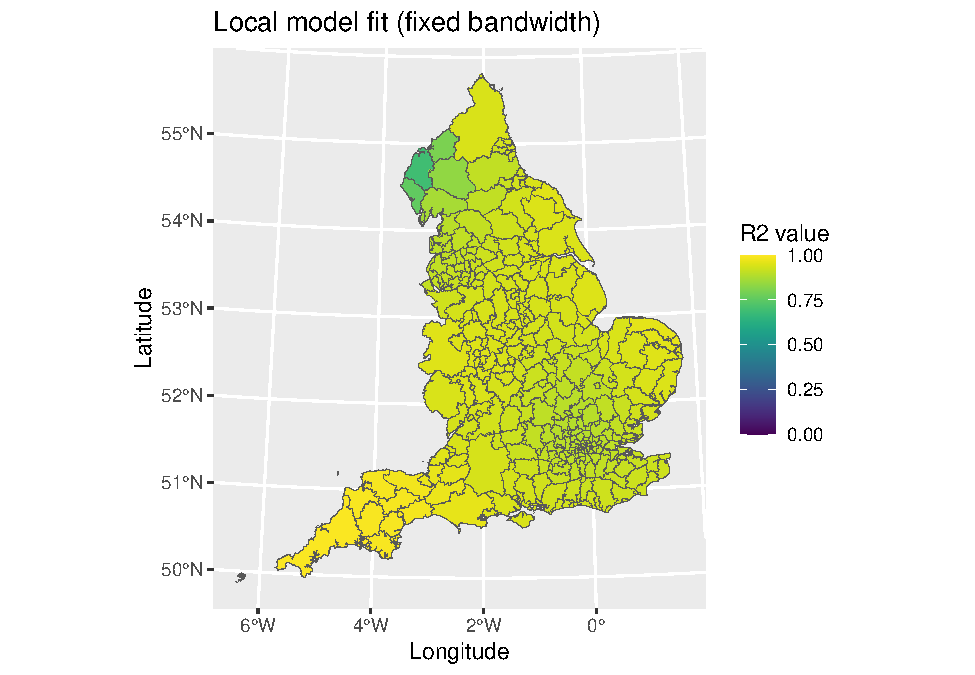
\includegraphics{Spatial-Data_files/figure-latex/unnamed-chunk-71-1.pdf}

Model fit looks good, but with poorer fit in the North West of England (e.g., Cumbria). Let's repeat this for the adaptive bandwidth model.

\begin{Shaded}
\begin{Highlighting}[]
\CommentTok{\# Tidy data}
\NormalTok{results\_adapt }\OtherTok{\textless{}{-}} \FunctionTok{as.data.frame}\NormalTok{(model2\_adapt}\SpecialCharTok{$}\NormalTok{SDF) }\CommentTok{\# Save coefficients}
\NormalTok{lad\_eng}\SpecialCharTok{$}\NormalTok{adapt\_r2 }\OtherTok{\textless{}{-}}\NormalTok{ results\_adapt}\SpecialCharTok{$}\NormalTok{localR2 }\CommentTok{\# Add local r2 value to data for mapping}

\CommentTok{\# Plot}
\NormalTok{map3 }\OtherTok{\textless{}{-}} \FunctionTok{ggplot}\NormalTok{() }\SpecialCharTok{+} \CommentTok{\# Call ggplot command}
  \FunctionTok{geom\_sf}\NormalTok{(}\AttributeTok{data =}\NormalTok{ lad\_eng, }\FunctionTok{aes}\NormalTok{(}\AttributeTok{fill =}\NormalTok{ adapt\_r2), }\AttributeTok{lwd =} \DecValTok{0}\NormalTok{) }\SpecialCharTok{+} \CommentTok{\# Define what to plot}
  \FunctionTok{scale\_fill\_viridis}\NormalTok{(}\AttributeTok{limits =} \FunctionTok{c}\NormalTok{(}\DecValTok{0}\NormalTok{, }\DecValTok{1}\NormalTok{)) }\SpecialCharTok{+} \CommentTok{\# Make colourblind friendly (and set limits to plot for consistency)}
  \FunctionTok{xlab}\NormalTok{(}\StringTok{"Longitude"}\NormalTok{) }\SpecialCharTok{+} \CommentTok{\# Add x{-}axis label}
  \FunctionTok{ylab}\NormalTok{(}\StringTok{"Latitude"}\NormalTok{) }\SpecialCharTok{+} \CommentTok{\# Add y{-}axis label}
  \FunctionTok{labs}\NormalTok{(}\AttributeTok{title =} \StringTok{"Local model fit (adaptive bandwidth)"}\NormalTok{, }\CommentTok{\# Edit plot title}
       \AttributeTok{fill =} \StringTok{"R2 value"}\NormalTok{) }\CommentTok{\# Edit legend title}
\NormalTok{map3 }\CommentTok{\# Print plot}
\end{Highlighting}
\end{Shaded}

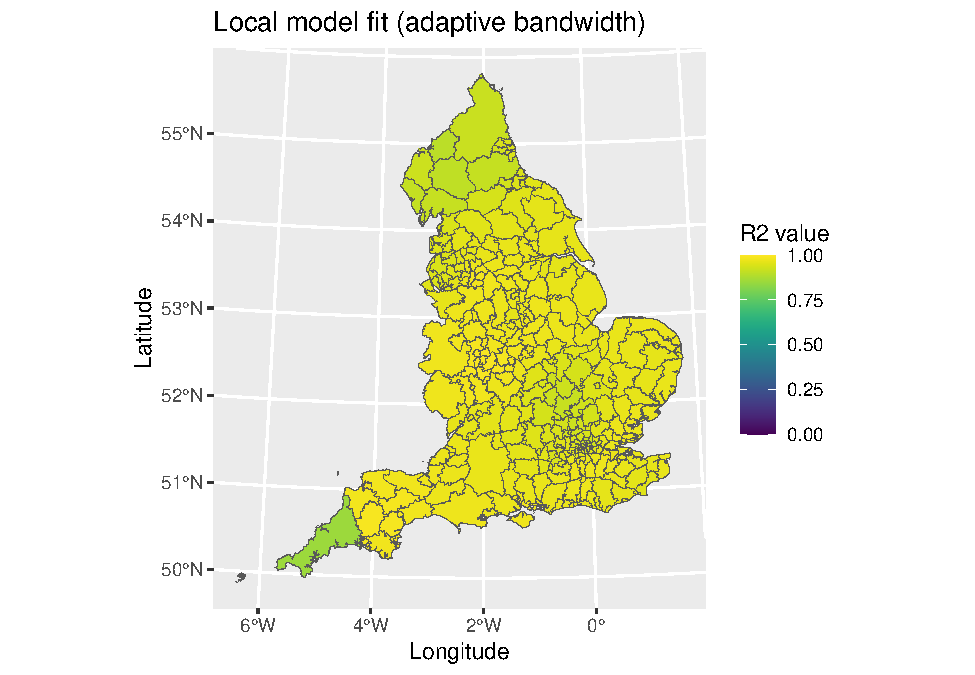
\includegraphics{Spatial-Data_files/figure-latex/unnamed-chunk-72-1.pdf}

There is some poorer fit in the Northern England and in Cornwall, but otherwise it looks fairly good.

In sum, both of the models are very good. For the purposes of this tutorial, we will use the adaptive bandwidth since it generally has better model fit.

\hypertarget{plotting-coefficients}{%
\subsection{Plotting coefficients}\label{plotting-coefficients}}

Let's begin through looking at our overall summary of our analytical model. We can print out the raw output just by running the object in R. I don't know of a way of cleaning this into a nice and tidy table \sout{sorry, not sorry}.

\begin{Shaded}
\begin{Highlighting}[]
\NormalTok{model2\_fixed}
\end{Highlighting}
\end{Shaded}

\begin{verbatim}
## Call:
## gwr(formula = percent_second_dose ~ median_age + Other_White + 
##     Mixed + Black + Asian + Other + mean_imd_score + pop_density, 
##     data = lad_eng, coords = cbind(lad_eng$long, lad_eng$lat), 
##     bandwidth = fixed_bandwidth, hatmatrix = TRUE, longlat = TRUE, 
##     se.fit = TRUE)
## Kernel function: gwr.Gauss 
## Fixed bandwidth: 46.81257 
## Summary of GWR coefficient estimates at data points:
##                       Min.     1st Qu.      Median     3rd Qu.        Max.  Global
## X.Intercept.   -2.4903e+01 -9.1887e-01  3.0533e+00  7.3111e+00  1.3355e+02  4.7973
## median_age     -1.1969e+00  9.7545e-01  1.0405e+00  1.1616e+00  1.6200e+00  1.0410
## Other_White    -3.3888e-01 -1.7318e-01 -1.6598e-02  7.1306e-02  7.6619e-01 -0.1071
## Mixed          -6.5502e-01  1.0532e-02  3.6080e-01  4.9383e-01  4.1734e+00  0.1229
## Black          -1.8214e+01 -4.1662e-01 -2.3640e-01 -1.3846e-01 -6.8347e-03 -0.1811
## Asian          -5.2151e+00 -7.6231e-02 -7.4432e-03  5.8227e-03  6.5581e-02 -0.0260
## Other          -9.0439e+00 -1.8882e-01 -1.0064e-01  1.1253e-01  3.0705e+00 -0.1225
## mean_imd_score -7.8441e-01 -5.0281e-02  1.0860e-02  6.3091e-02  2.0162e-01  0.0205
## pop_density    -7.9592e-04 -7.3941e-04 -5.5343e-05  2.9945e-04  7.5985e-03 -0.0004
## Number of data points: 317 
## Effective number of parameters (residual: 2traceS - traceS'S): 94.59721 
## Effective degrees of freedom (residual: 2traceS - traceS'S): 222.4028 
## Sigma (residual: 2traceS - traceS'S): 2.160288 
## Effective number of parameters (model: traceS): 72.72148 
## Effective degrees of freedom (model: traceS): 244.2785 
## Sigma (model: traceS): 2.06129 
## Sigma (ML): 1.809473 
## AICc (GWR p. 61, eq 2.33; p. 96, eq. 4.21): 1468.508 
## AIC (GWR p. 96, eq. 4.22): 1348.313 
## Residual sum of squares: 1037.919 
## Quasi-global R2: 0.9411265
\end{verbatim}

There is a lot of output and information here. Let's just focus on the summary of the GWR coefficients, which is typically what would be reported in a report. The table presents summary statistics for the coefficients in the model (each coefficient is a row) across all of the local regressions (in our case, all 317 regression models). We may be interested in the minimum and maximum values to see what the range of values are (which is a useful first step to see if coefficients vary in direction). The global model is the same as OLS coefficients and is a useful point of reference to compare to estimates generated in the GWR model. The 1st Quartile, Median and 3rd Quartile values are also useful for considering the variation in values in terms of direction of association and magnitude of strength.

The next step will be to visualise the spatial variations in coefficient values. This will allow us to see if there are any distinct geographical patterns in relationships. We will just plot for the variable IMD score (deprivation). First, let's plot the coefficient values.

\begin{Shaded}
\begin{Highlighting}[]
\CommentTok{\# Get data}
\NormalTok{lad\_eng}\SpecialCharTok{$}\NormalTok{imd\_coef }\OtherTok{\textless{}{-}}\NormalTok{ model2\_fixed}\SpecialCharTok{$}\NormalTok{SDF}\SpecialCharTok{$}\NormalTok{mean\_imd\_score }\CommentTok{\# Coefficients}

\CommentTok{\# Plot}
\NormalTok{map4 }\OtherTok{\textless{}{-}} \FunctionTok{ggplot}\NormalTok{() }\SpecialCharTok{+} \CommentTok{\# Call ggplot command}
  \FunctionTok{geom\_sf}\NormalTok{(}\AttributeTok{data =}\NormalTok{ lad\_eng, }\FunctionTok{aes}\NormalTok{(}\AttributeTok{fill =}\NormalTok{ imd\_coef), }\AttributeTok{lwd =} \DecValTok{0}\NormalTok{) }\SpecialCharTok{+} \CommentTok{\# Define what to plot}
  \FunctionTok{scale\_fill\_viridis}\NormalTok{() }\SpecialCharTok{+} \CommentTok{\# Make colourblind friendly}
  \FunctionTok{xlab}\NormalTok{(}\StringTok{"Longitude"}\NormalTok{) }\SpecialCharTok{+} \CommentTok{\# Add x{-}axis label}
  \FunctionTok{ylab}\NormalTok{(}\StringTok{"Latitude"}\NormalTok{) }\SpecialCharTok{+} \CommentTok{\# Add y{-}axis label}
  \FunctionTok{labs}\NormalTok{(}\AttributeTok{title =} \StringTok{"Deprivation"}\NormalTok{, }\CommentTok{\# Edit plot title}
       \AttributeTok{fill =} \StringTok{"Coefficient"}\NormalTok{) }\CommentTok{\# Edit legend title}
\NormalTok{map4 }\CommentTok{\# Print plot}
\end{Highlighting}
\end{Shaded}

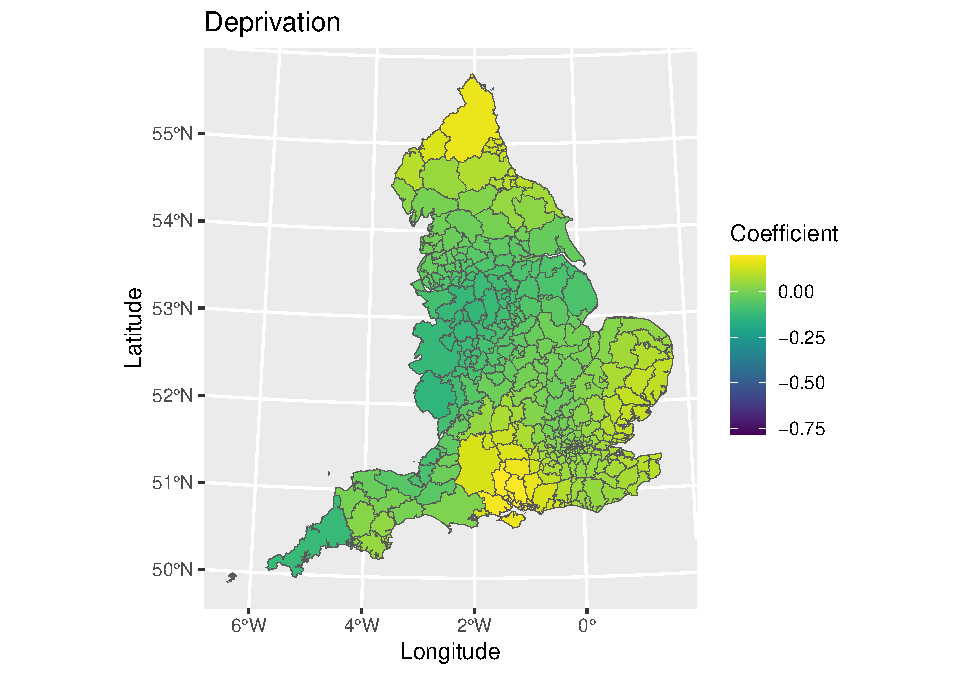
\includegraphics{Spatial-Data_files/figure-latex/unnamed-chunk-74-1.pdf}

We may also want to plot the standard errors to look at the variability in the precision of our coefficient estimates.

\begin{Shaded}
\begin{Highlighting}[]
\CommentTok{\# Get data}
\NormalTok{lad\_eng}\SpecialCharTok{$}\NormalTok{imd\_coef\_se }\OtherTok{\textless{}{-}}\NormalTok{ model2\_fixed}\SpecialCharTok{$}\NormalTok{SDF}\SpecialCharTok{$}\NormalTok{mean\_imd\_score\_se }\CommentTok{\# Standard error}

\CommentTok{\# Plot}
\NormalTok{map5 }\OtherTok{\textless{}{-}} \FunctionTok{ggplot}\NormalTok{() }\SpecialCharTok{+} \CommentTok{\# Call ggplot command}
  \FunctionTok{geom\_sf}\NormalTok{(}\AttributeTok{data =}\NormalTok{ lad\_eng, }\FunctionTok{aes}\NormalTok{(}\AttributeTok{fill =}\NormalTok{ imd\_coef\_se), }\AttributeTok{lwd =} \DecValTok{0}\NormalTok{) }\SpecialCharTok{+} \CommentTok{\# Define what to plot}
  \FunctionTok{scale\_fill\_viridis}\NormalTok{() }\SpecialCharTok{+} \CommentTok{\# Make colourblind friendly}
  \FunctionTok{xlab}\NormalTok{(}\StringTok{"Longitude"}\NormalTok{) }\SpecialCharTok{+} \CommentTok{\# Add x{-}axis label}
  \FunctionTok{ylab}\NormalTok{(}\StringTok{"Latitude"}\NormalTok{) }\SpecialCharTok{+} \CommentTok{\# Add y{-}axis label}
  \FunctionTok{labs}\NormalTok{(}\AttributeTok{title =} \StringTok{"Deprivation"}\NormalTok{, }\CommentTok{\# Edit plot title}
       \AttributeTok{fill =} \StringTok{"Standard Error"}\NormalTok{) }\CommentTok{\# Edit legend title}
\NormalTok{map5 }\CommentTok{\# Print plot}
\end{Highlighting}
\end{Shaded}

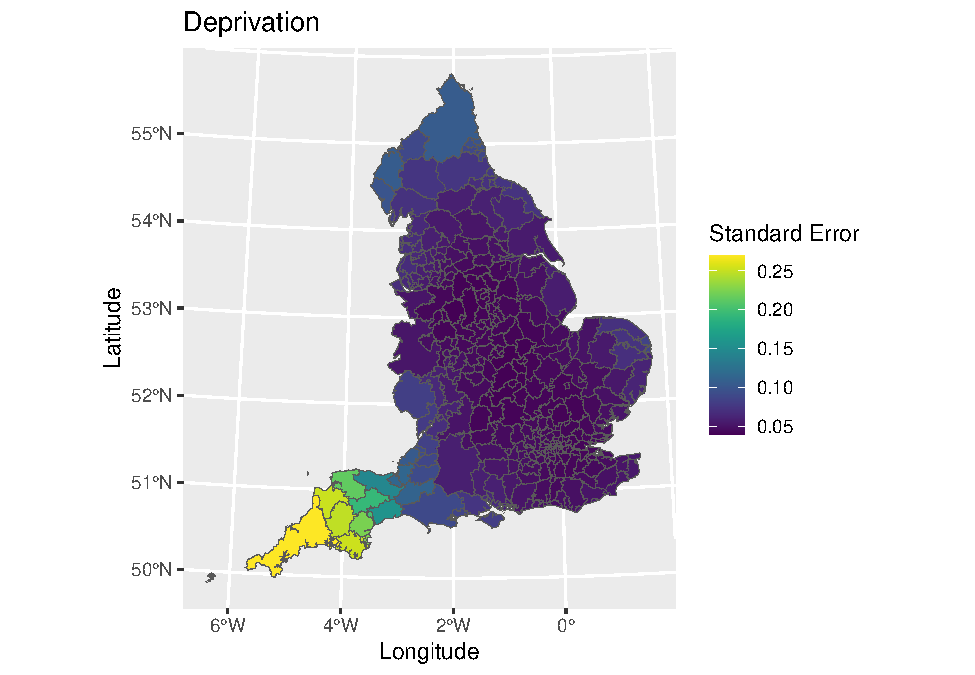
\includegraphics{Spatial-Data_files/figure-latex/unnamed-chunk-75-1.pdf}

The next step would be to assess the statistical significance of the coefficients to identify if any associations were meaningful. To do this, we estimate the t-value and then categorise observations if they meet 95\% level of significance. Let's plot areas based on whether they meet the criterion.

\begin{Shaded}
\begin{Highlighting}[]
\CommentTok{\# Calculate t statistic}
\NormalTok{lad\_eng}\SpecialCharTok{$}\NormalTok{t\_imd\_coef }\OtherTok{=}\NormalTok{ results\_fixed}\SpecialCharTok{$}\NormalTok{mean\_imd\_score }\SpecialCharTok{/}\NormalTok{ results\_fixed}\SpecialCharTok{$}\NormalTok{mean\_imd\_score\_se}

\CommentTok{\# Categorise t values as significant or not}
\NormalTok{lad\_eng}\SpecialCharTok{$}\NormalTok{t\_imd\_coef\_cat }\OtherTok{\textless{}{-}} \FunctionTok{cut}\NormalTok{(lad\_eng}\SpecialCharTok{$}\NormalTok{t\_imd\_coef,}
                     \AttributeTok{breaks=}\FunctionTok{c}\NormalTok{(}\FunctionTok{min}\NormalTok{(lad\_eng}\SpecialCharTok{$}\NormalTok{t\_imd\_coef), }\SpecialCharTok{{-}}\DecValTok{2}\NormalTok{, }\DecValTok{2}\NormalTok{, }\FunctionTok{max}\NormalTok{(lad\_eng}\SpecialCharTok{$}\NormalTok{t\_imd\_coef)),}
                     \AttributeTok{labels=}\FunctionTok{c}\NormalTok{(}\StringTok{"Sig."}\NormalTok{,}\StringTok{"Non{-}sig."}\NormalTok{, }\StringTok{"Sig."}\NormalTok{))}

\CommentTok{\# Plot}
\NormalTok{map6 }\OtherTok{\textless{}{-}} \FunctionTok{ggplot}\NormalTok{() }\SpecialCharTok{+} \CommentTok{\# Call ggplot command}
  \FunctionTok{geom\_sf}\NormalTok{(}\AttributeTok{data =}\NormalTok{ lad\_eng, }\FunctionTok{aes}\NormalTok{(}\AttributeTok{fill =}\NormalTok{ t\_imd\_coef\_cat), }\AttributeTok{lwd =} \DecValTok{0}\NormalTok{) }\SpecialCharTok{+} \CommentTok{\# Define what to plot}
  \FunctionTok{scale\_fill\_viridis\_d}\NormalTok{() }\SpecialCharTok{+} \CommentTok{\# Make colourblind friendly}
  \FunctionTok{xlab}\NormalTok{(}\StringTok{"Longitude"}\NormalTok{) }\SpecialCharTok{+} \CommentTok{\# Add x{-}axis label}
  \FunctionTok{ylab}\NormalTok{(}\StringTok{"Latitude"}\NormalTok{) }\SpecialCharTok{+} \CommentTok{\# Add y{-}axis label}
  \FunctionTok{labs}\NormalTok{(}\AttributeTok{title =} \StringTok{"Deprivation"}\NormalTok{, }\CommentTok{\# Edit plot title}
       \AttributeTok{fill =} \StringTok{"Statistical significance"}\NormalTok{) }\CommentTok{\# Edit legend title}
\NormalTok{map6 }\CommentTok{\# Print plot}
\end{Highlighting}
\end{Shaded}

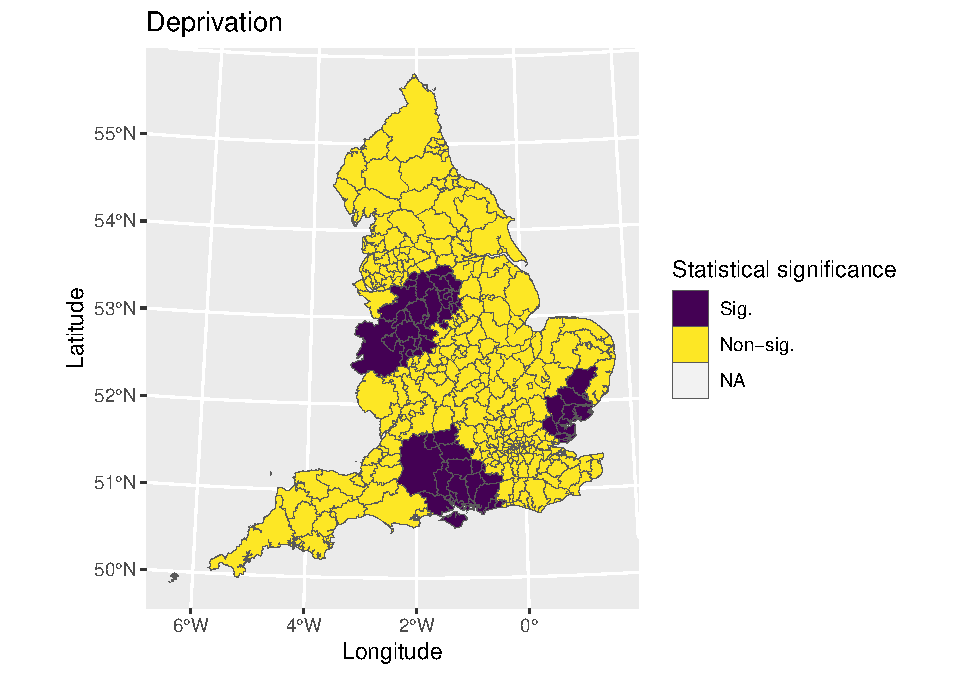
\includegraphics{Spatial-Data_files/figure-latex/unnamed-chunk-76-1.pdf}

It may be useful to combine the coefficient and statistical significance plots into one single visualisation. You could do this by joining the two plots together side-by-side using a R package like \texttt{patchwork}. Rather, we will only plot significant associations and hide those which are not.

\begin{Shaded}
\begin{Highlighting}[]
\CommentTok{\# Plot}
\NormalTok{map7 }\OtherTok{\textless{}{-}} \FunctionTok{ggplot}\NormalTok{() }\SpecialCharTok{+} \CommentTok{\# Call ggplot command}
    \FunctionTok{geom\_sf}\NormalTok{(}\AttributeTok{data =}\NormalTok{ lad\_eng, }\AttributeTok{lwd =} \DecValTok{0}\NormalTok{) }\SpecialCharTok{+} \CommentTok{\# Plot all areas as base layer}
    \FunctionTok{geom\_sf}\NormalTok{(}\AttributeTok{data =}\NormalTok{ lad\_eng[lad\_eng}\SpecialCharTok{$}\NormalTok{t\_imd\_coef\_cat }\SpecialCharTok{==} \StringTok{"Sig."}\NormalTok{,], }\FunctionTok{aes}\NormalTok{(}\AttributeTok{fill =}\NormalTok{ imd\_coef), }\AttributeTok{lwd =} \DecValTok{0}\NormalTok{) }\SpecialCharTok{+} \CommentTok{\# Plot the coefficients that are significant}
    \FunctionTok{scale\_fill\_viridis}\NormalTok{() }\SpecialCharTok{+} \CommentTok{\# Make colourblind friendly}
    \FunctionTok{xlab}\NormalTok{(}\StringTok{"Longitude"}\NormalTok{) }\SpecialCharTok{+} \CommentTok{\# Add x{-}axis label}
    \FunctionTok{ylab}\NormalTok{(}\StringTok{"Latitude"}\NormalTok{) }\SpecialCharTok{+} \CommentTok{\# Add y{-}axis label}
    \FunctionTok{labs}\NormalTok{(}\AttributeTok{title =} \StringTok{"Deprivation"}\NormalTok{, }\CommentTok{\# Edit plot title}
         \AttributeTok{fill =} \StringTok{"Coefficient"}\NormalTok{) }\CommentTok{\# Edit legend title}
\NormalTok{map7 }\CommentTok{\# Print plot}
\end{Highlighting}
\end{Shaded}

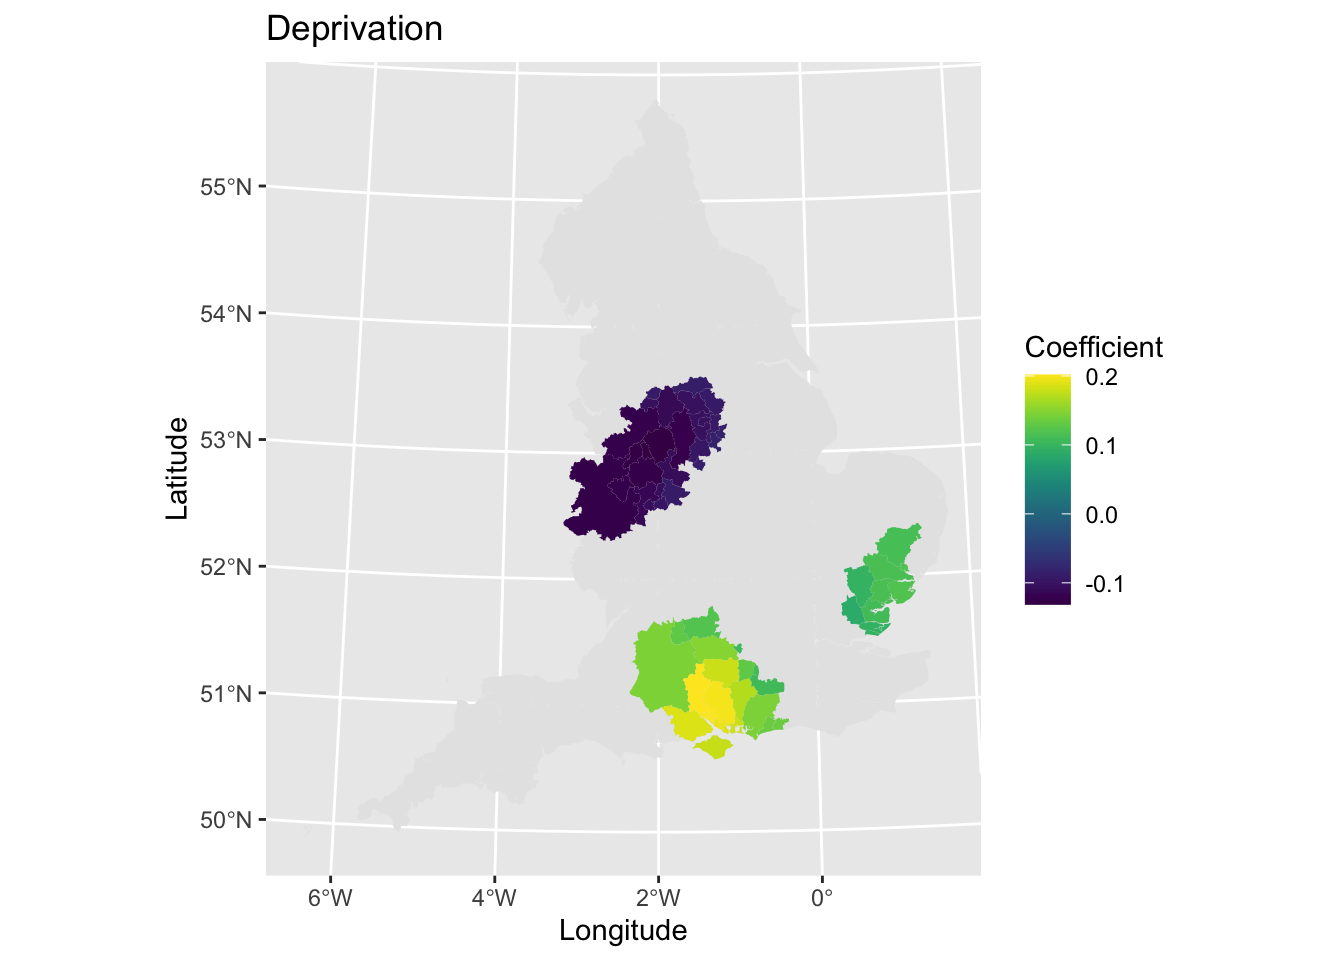
\includegraphics{Spatial-Data_files/figure-latex/unnamed-chunk-77-1.pdf}

Why not have a look at other coefficients now - what can you find out? What interesting spatial patterns are there?

\hypertarget{scaling-gwr-for-large-datasets}{%
\section{Scaling GWR for large datasets}\label{scaling-gwr-for-large-datasets}}

GWR models are computationally intensive to fit and therefore do not scale well with larger datasets (even those with 10000+ observations can be demanding). Some clever cookies have adapted the methodology to estimate the model quicker when dealing with larger or more complex datasets, including creating the R package \texttt{scgwr} (SCalable GWR) to implement the method in R. You can read more about the methodology \href{https://www.tandfonline.com/doi/full/10.1080/24694452.2020.1774350}{here}.

The actual code is not too difficult to use, but may require some refinement to model parameters. Specifically, we may want to play about with:

\begin{itemize}
\tightlist
\item
  \texttt{knn} - Number of nearest-neighbours selected during estimation: larger is better for bigger datasets.
\item
  \texttt{nsamp} - Number of random samples for (aproximate) cross-validation: should be smaller than sample size, but larger is better for minimising errors due to random sampling.
\end{itemize}

Let's re-run the model again, but using the \texttt{scgwr} package. Unfortunately, this code does not work with our example so I leave it in here to show the option for you in case you ever need it. If you can fix it, please send in your answers on a postcode.

\begin{Shaded}
\begin{Highlighting}[]
\CommentTok{\# \# Library}
\CommentTok{\# library(scgwr)}
\CommentTok{\# }
\CommentTok{\# \# Tidy data}
\CommentTok{\# outcome \textless{}{-} lad\_eng[, "percent\_second\_dose"] \# Store outcome variable (if don\textquotesingle{}t define as object then stores as list)}
\CommentTok{\# xvars \textless{}{-} lad\_eng[, c("median\_age", "Other\_White", "Mixed", "Black", "Asian", "Other", "mean\_imd\_score", "pop\_density")] \# Store explanatory variables}
\CommentTok{\# xy \textless{}{-} lad\_eng[, c("long", "lat")] \# Store co{-}ordinates}
\CommentTok{\# }
\CommentTok{\# \# Model}
\CommentTok{\# model3 \textless{}{-} scgwr(y = outcome, x = xvars, coords = xy, knn = 100, kernel = "gau", p = 4, approach = "CV") \# Model using cross{-}validation approach ("CV") and Gaussian kernel ("gau")}
\end{Highlighting}
\end{Shaded}

The R package can incorporate parallel processing for faster processing as well using the \texttt{scgwr\_p} command.

\hypertarget{summary-3}{%
\section{Summary}\label{summary-3}}

In this practical session, we have explored how use Geographically Weighted Regression and explored the opportunities that it can bring for exploring spatially varying contexts.

\hypertarget{summary}{%
\chapter{Summary}\label{summary}}

Well done on making it to the end! Before we sign off, it is a good time to reflect over everything you have achieved over the past few weeks.

\hypertarget{learning-outcomes-1}{%
\section{Learning outcomes}\label{learning-outcomes-1}}

Let's review how you have achieved each of the learning outcomes for this section of the module.

\begin{enumerate}
\def\labelenumi{\arabic{enumi}.}
\tightlist
\item
  Produce static and interactive visualisations of spatial data.
\end{enumerate}

In the \protect\hyperlink{intro}{first session}, you learned how to load spatial data into R and map the data using a variety of packages. You produced different types of maps, including how to present them effectively or make maps interactive.

\begin{enumerate}
\def\labelenumi{\arabic{enumi}.}
\setcounter{enumi}{1}
\tightlist
\item
  Identify clustering of point- and area-based data.
\end{enumerate}

Our \protect\hyperlink{cluster}{second session} looked at how we might try to identify spatial clusters for data. First, descriptive techniques were applied on point-based data. Second, using area-based data you calculated spatial weights and looked for clusters using Moran's I approaches.

\begin{enumerate}
\def\labelenumi{\arabic{enumi}.}
\setcounter{enumi}{2}
\tightlist
\item
  Extend regression-based approaches to incorporate spatial context.
\end{enumerate}

The final learning outcome was achieved through two sessions. First, we extended OLS regression approaches using spatially lagged variables or accounted for the spatial structure of error terms to accommodate \protect\hyperlink{spatreg}{spatial regression techniques}. Second, we extended OLS regression approaches to incorporate spatially varying coefficients through \protect\hyperlink{gwr}{Geographically Weighted Regression}.

\hypertarget{further-learning}{%
\section{Further learning}\label{further-learning}}

The methods we have covered so far will have given you a good grounding in spatial methods, however they are just a small flavour of the vast range of opportunities thinking spatially can bring to research. Here are a few other areas or methods you can read up on in case you want to take things forward. For each, I have provided a (open access) research example of its application and some example R code/packages for you to see how it can be done.

\begin{itemize}
\tightlist
\item
  \textbf{Cartograms} -\textgreater{} \emph{Description:} Maps can lie. They can distort patterns, resulting in the misleading interpretation of data. One distortion comes from the geographical size of zones. Where zones are small they can be hard to see, and hence larger areas may attract your attention. You may have noticed this in the \protect\hyperlink{spatreg}{spatial regression session} when some cities were difficult to see on the maps. Cartograms (including linked methods for distorting area sizes such as hexmaps) offer one way of minimising this bias, through readjusting the geographical sizes of areas based on their underlying population sizes. This can allow for fairer comparisons, especially when mapping \emph{people} rather than \emph{places}. \emph{Research example:} \href{https://journals.plos.org/plosmedicine/article?id=10.1371/journal.pmed.0040001}{Worldmapper: The Human Anatomy of a Small Planet}. \emph{R example:} \href{https://r-charts.com/spatial/cartogram-ggplot2/}{Tutorial using ggplot2}.
\item
  \textbf{Spatial panel model} -\textgreater{} \emph{Description:} The spatial regression models we have introduced are cross-sectional (i.e., a single point in time) and can not account for the longitudinal nature of datasets (i.e., where we have repeated data points over time for each area). These models can be extended longitudinally, similar to how we might extend the classical regression model to incorporate time, to give stronger tests of associations between predictors and outcomes. \emph{Research example:} \href{https://www.ncbi.nlm.nih.gov/pmc/articles/PMC7139267/}{Determining the spatial effects of COVID-19 using the spatial panel data model}. \emph{R example:} \href{http://www.jstatsoft.org/v47/i01/}{Package spml}.
\item
  \textbf{Spatial multi-level} -\textgreater{} \emph{Description:} Multi-level modelling revolutionised health geography, since through nesting individuals within areas you could control for individual level characteristics and, in theory, separate out differences which difference between areas can explain. While these methods are powerful, they do not explicitly account for space since the model does not which areas are located where. There exists spatial extensions to multi-level models. \emph{Research example:} \href{https://journals.plos.org/plosone/article?id=10.1371/journal.pone.0130761}{Methodological paper extending multi-level models to incoporate spatial effects}. \emph{R example:} \href{https://cran.r-project.org/web/packages/HSAR/HSAR.pdf}{HSAR package}.
\item
  \textbf{Spatial interaction models and flow data} -\textgreater{} \emph{Description:} Flow data are not frequently found in spatial health research. They refer to where we have observations of spatial interactions between two places. The most common application might be movement data (e.g., in- and out-migration flows between two places). Spatial interaction models extend these data and organise them into a regression framework, that can model the interactions between places to understand what may drive them. \emph{Research example:} \href{https://www.mdpi.com/2071-1050/9/11/1924}{Using a Spatial Interaction Model to Assess the Accessibility of District Parks in Hong Kong}. \emph{R example:} \href{https://rpubs.com/adam_dennett/257231}{Spatial Interaction Models for Dummies}.
\item
  \textbf{Location-allocation} -\textgreater{} \emph{Description:} Where we have spatial points representing sites/locations (e.g., health services), we can try to geographically optimise the locations of sites to improve geographical coverage. This can be useful for locating new site locations, including finding where it is best to place new sites to maximise coverage in areas with low access. \emph{Research example:} \href{https://extra.shu.ac.uk/ppp-online/wp-content/uploads/2021/04/thinking-spatially-roll-out-testing-liverpool.pdf}{Evaluating the locations of asymptomatic COVID-19 test sites in Liverpool}. \emph{R example:} \href{https://github.com/markagreen/mapping_test_accessibility/blob/main/scripts/location_allocation_model.R}{Replicatable code from research example}.
\item
  \textbf{Bayesian extensions} -\textgreater{} \emph{Description:} Bayesian models offer an alternative approach to analysis than frequentist methods. There are a lot of different spatial extensions to Bayesian models, allowing for more flexibility to how we approach our analyses. These approaches are important if we want to utilise generalised linear models. \emph{Research example:} \href{https://www.sciencedirect.com/science/article/pii/S2666776221000843}{Evaluating social and spatial inequalities in COVID-19 testing in Liverpool}. \emph{R example:} \href{https://www.paulamoraga.com/book-geospatial/}{Geospatial Health Data Book}.
\item
  \textbf{Causal inference methods} -\textgreater{} \emph{Description:} There are a large number of techniques that have tried to implement causal inference approaches within a spatial framework. One example of these methods might be spatial regression discontinuity approaches, where you assess impacts of interventions in places through comparisons to the impacts closest to them where they were not implemented. \emph{Research example:} \href{https://arxiv.org/abs/2007.02714}{Review of spatial causal inference methods}. \emph{R example:} \href{https://github.com/axlehner/SpatialRDD}{SpatialRDD package}.
\item
  \textbf{Spatial machine learning} -\textgreater{} \emph{Description:} A relatively newer area of research explores how we can extend machine learning methods to explicitly incorporate space into them. This field is so new that I have very little to report here! \emph{Research example:} \href{https://www.nature.com/articles/s41598-020-79148-7}{Spatio-temporal predictions using deep learning}. \emph{R example:} \href{https://geocompr.robinlovelace.net/spatial-cv.html}{Statistical Learning tutorial}.
\end{itemize}

\hypertarget{thank-you}{%
\section{Thank you}\label{thank-you}}

I would just like to end by thanking you for taking the time to read through these materials and hopefully you have enjoyed learning about spatial data analysis. If you have any further questions, please do not hesitate to get in contact.

Dr Mark A. Green\\
Senior Lecturer in Health Geography\\
University of Liverpool\\
\href{mailto:mark.green@liverpool.ac.uk}{\nolinkurl{mark.green@liverpool.ac.uk}}

  \bibliography{book.bib,packages.bib}

\end{document}
